%%____________________________________________________________________________||
\section{Systematic uncertainties in the \mht dimension}
\label{sec:syst-on-shape}

The estimate of the number of events per (\njet,\nb,\scalht) bin,
integrated over \mht, is derived from data control samples, with
the associated systematic error determined from closure tests
described in Section \ref{sec:syst-from-closure}. This section
describes the method used to assess the systematic uncertainties in
the distribution of events according to \mht. A data driven approach is
utilised under the hypothesis of zero bias in the data and MC agreement.
The level of closure in the control regions is used
to derive alternative templates accounting for systematic uncertainties.

When looking at the \mht dimension inclusively in \scalht there are
large theoretical uncertainties that originate from mixing events
at different scales. These uncertainties can be mitigated if the events 
are binned according to a variable, such as \scalht, 
which is strongly correlated with the scale of the event. 
After this categorisation is applied, the uncertainty in 
the distribution of the \mht variable
(as well as any other MET-like variable) is expected to be 
mainly affected by the MC modelling of the particle 
decays and, to a lesser extent, by jet reconstruction effects, 
such as jet energy scale and resolution. 
This approach, which will be often referred to as \textit{scale anchoring}
in the following, is used in this analysis. The distribution in \mht
is measured in data using the control regions and compared to MC
to determine the validity of the zero bias hypothesis after scale anchoring.

In Section~\ref{sec:valid8} the 8 \TeV data will be used 
to validate the scale anchoring approach. 
In Section~\ref{sec:systMhtDimension} 
the procedure used to extract the systematic uncertainties in the 
\mht dimension is described and results shown with 8 \TeV data. 
In Section~\ref{sec:dataValid13TeV} the validation is repeated with 13\TeV data
and in Section~\ref{sec:biasInj} the results of a bias injection test described.
Finally, in \ref{sec:syst13TeV} the expected systematics for 3\ifb in Run 2 are be shown. 


% extent to which the control regions can constrain this bias 
% to the flat hypothesis
%Motivated by the inclusive distribution, a linear bias is assumed.

\subsection{Validation with 8 \texorpdfstring{\TeV} Data}
\label{sec:valid8}
In previous versions of this analysis three control regions
were used: \mj, \mmj and \gj. To parameterise the data/MC agreement
orthogonal polynomials are used such that odd and even powers 
are decorrelated \cite{cohen2013applied}. 
The $n^{th}$ order orthogonal polynomial which is fitted to the data/MC 
distribution is defined in Equation~\ref{equ:orthog-polynomial}.

\begin{equation}
  \label{equ:orthog-polynomial}
  f_n(x) = \sum_{k=0}^{k=n}{(p_k)\times(\bar{x}-x)^k}
\end{equation}

where $\bar{x}$ is the weighted mean of the distribution and $p_k = 0$ 
implies the $k^th$ order is negligible.
In Figure~\ref{fig:linearMotiv} the data/MC 
distribution against \mht for the control region selection 
(detailed in \cite{CMS_AN_2013-366}) is shown inclusive 
in \scalht and categories. By fitting a first order
orthogonal polynomial it can be seen that there is a large linear bias. 
This bias in the data/MC agreement is expected as events 
at different scales are mixed.
The first order orthogonal polynomial
will be used to measure the level of bias remaining 
when the \mht dimension is binned in \scalht.
This allows the normalisation parameter to be
decorrelated from the parameter which controls
the distribution in \mht.
The normalisation in each \scalht bin and its systematics 
is then fixed following the data-drived method used in Run 1. 
(Section~\ref{sec:systMhtDimension}).
\begin{figure}[h!]
  \centering
  \subfigure[\gj]{
    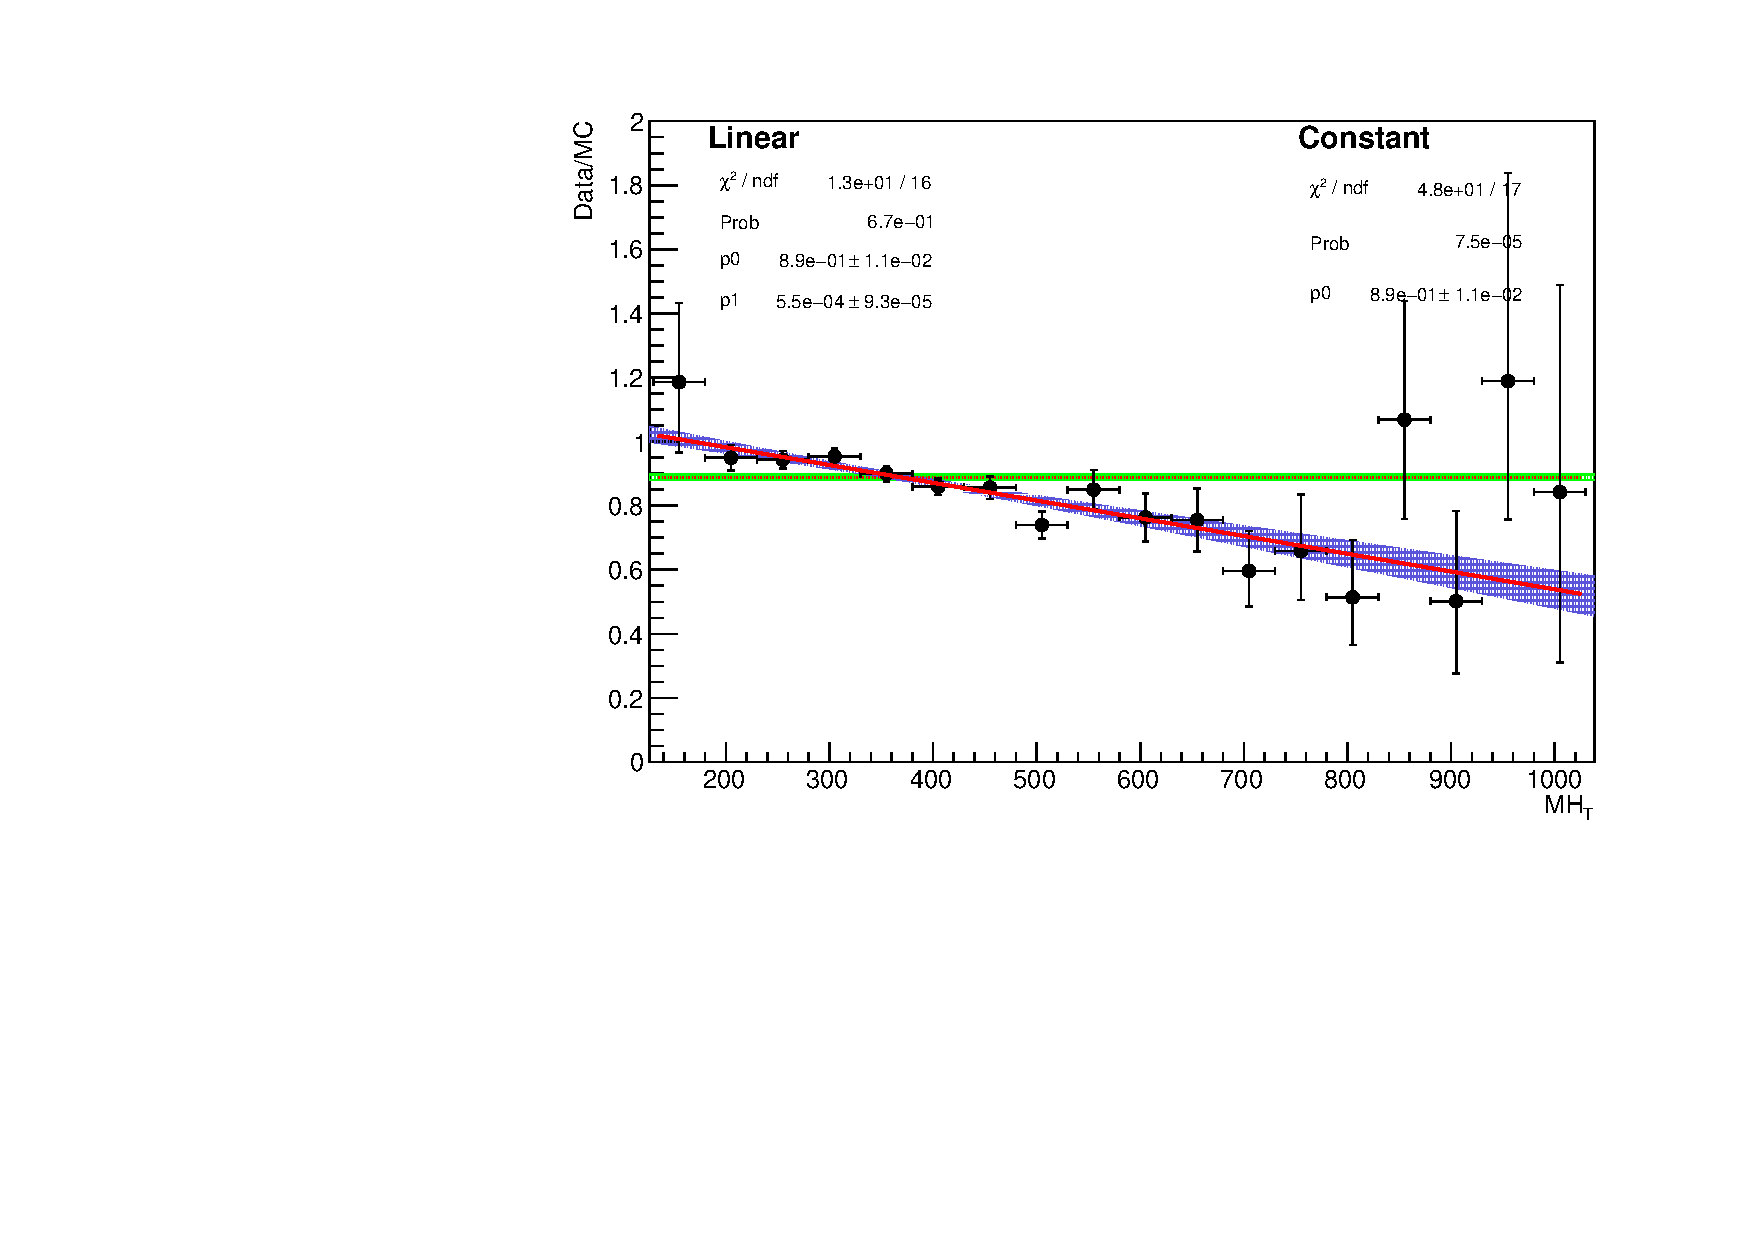
\includegraphics[width=0.5\textwidth]{figures/template/linear/mht_Inc_Inc_ht_Inc_SinglePhoton_Graph.pdf}
  }~~
  \subfigure[\mmj]{
    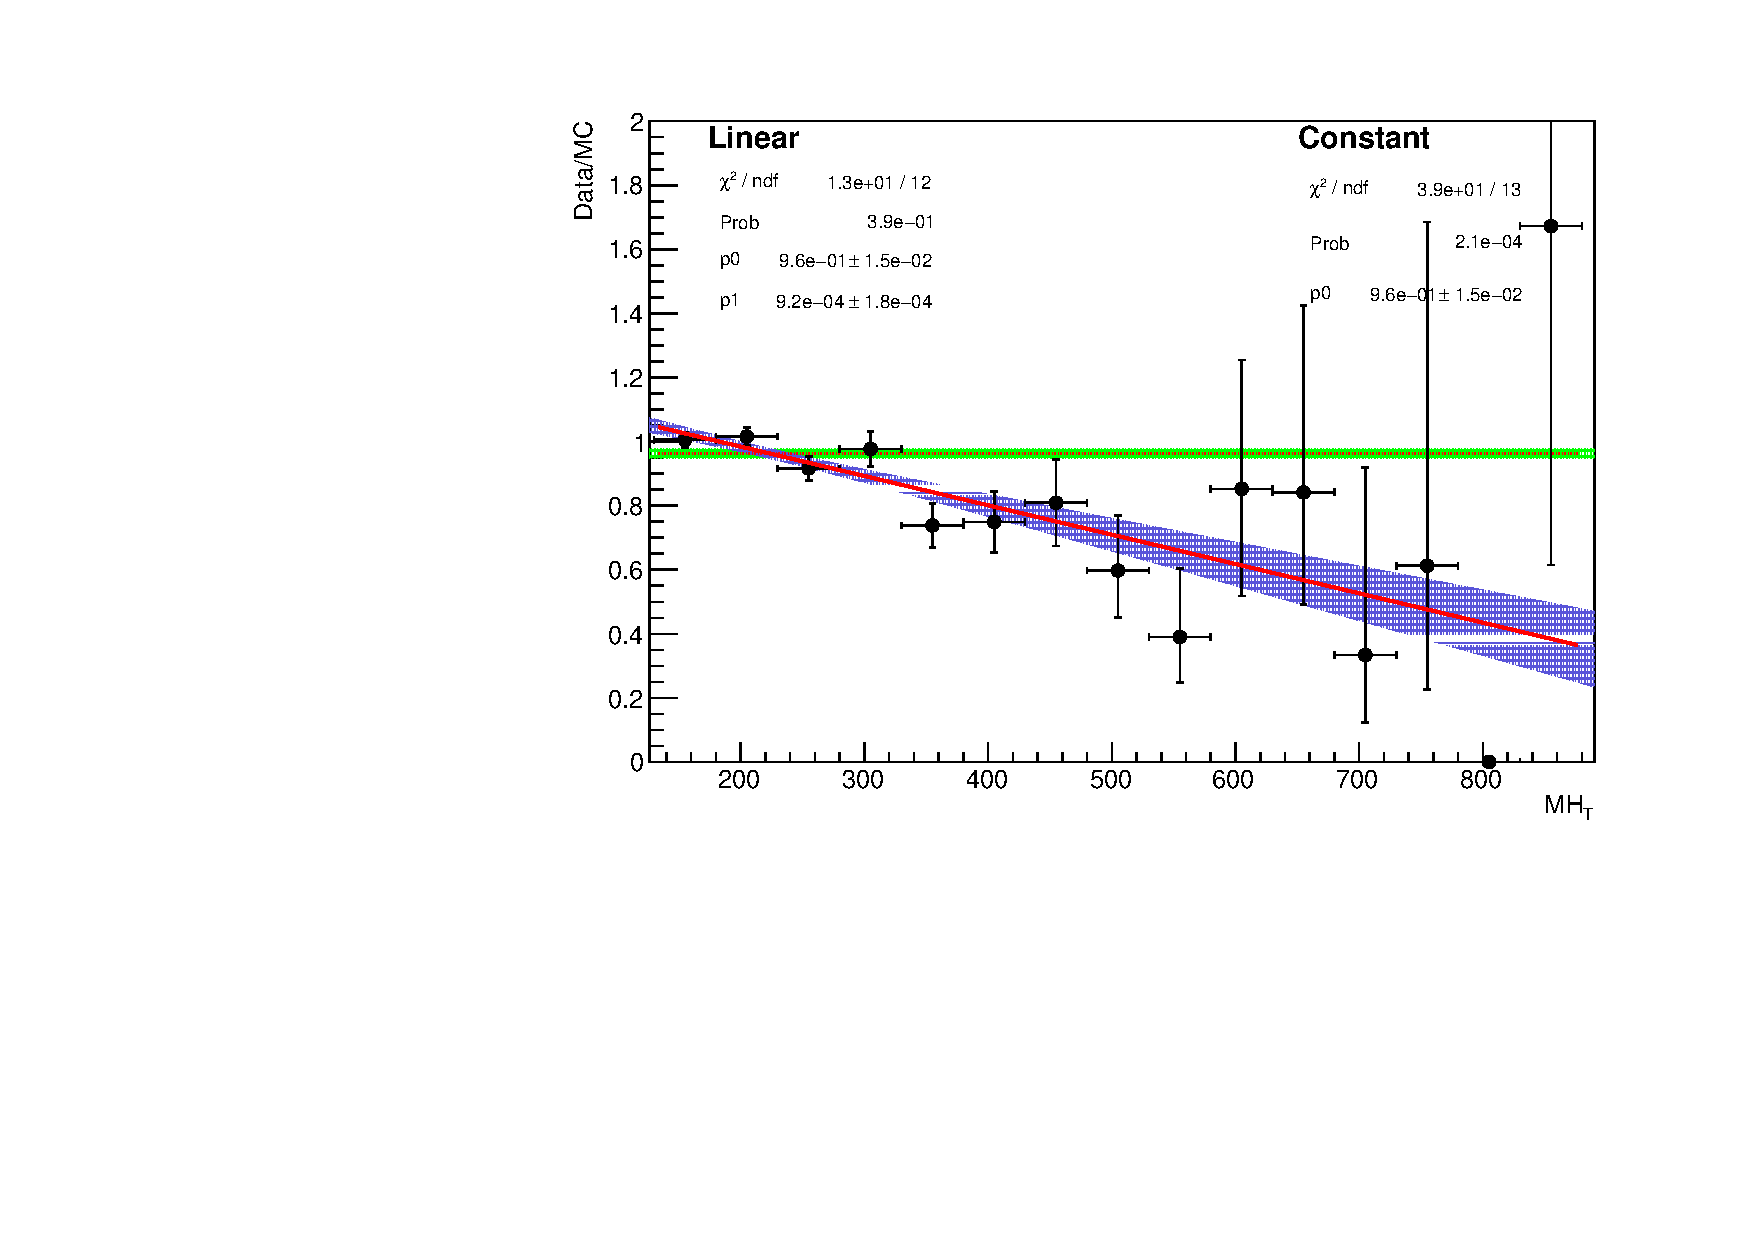
\includegraphics[width=0.5\textwidth]{figures/template/linear/mht_Inc_Inc_ht_Inc_DoubleMu_Graph.pdf}
  }\\
  \subfigure[\mj]{
    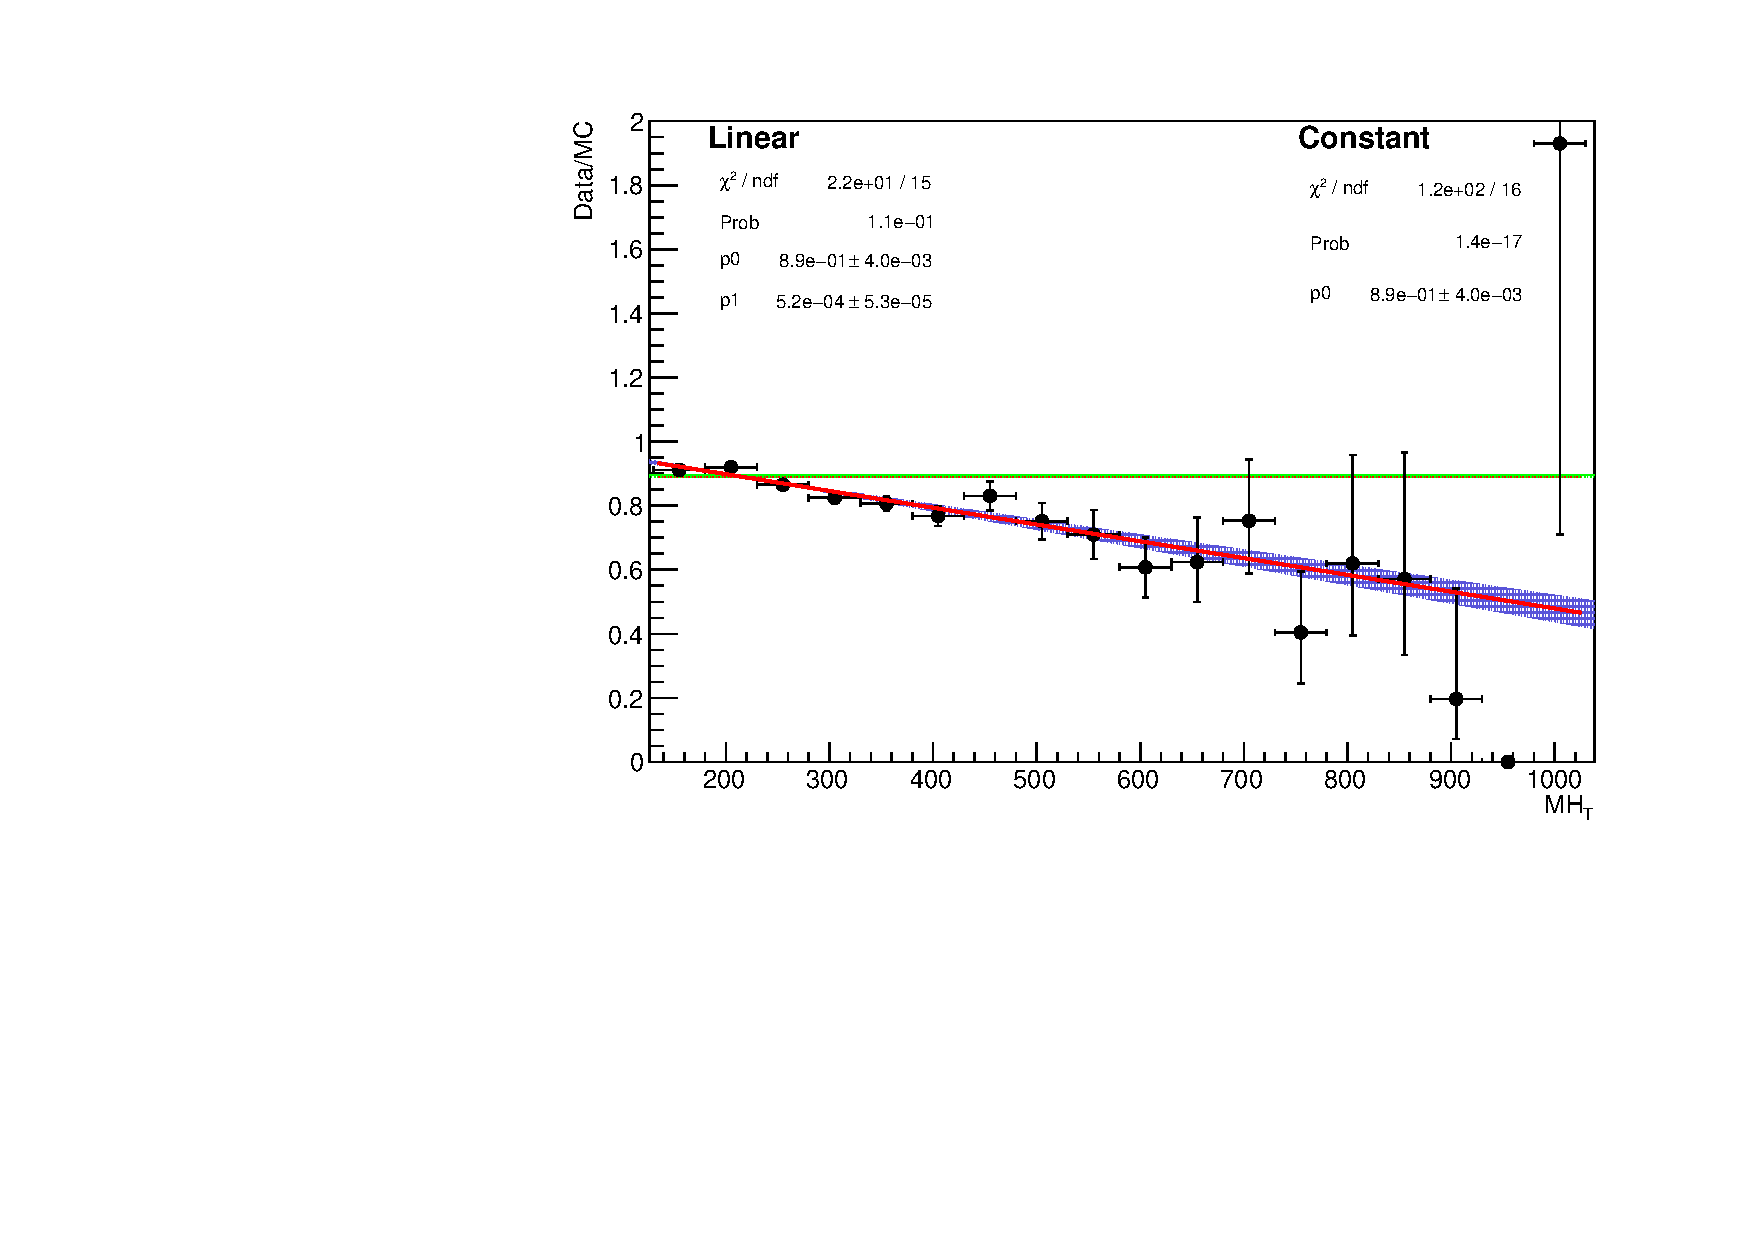
\includegraphics[width=0.5\textwidth]{figures/template/linear/mht_Inc_Inc_ht_Inc_SingleMu_Graph.pdf}
  }~~
  \\
  \caption{\label{fig:linearMotiv} 
  The data/MC distribution against \mht for an inclusive selection on category and \scalht
  showing the results of a linear fit. A large bias is observed. 
 }
\end{figure}

By anchoring the scale using binning in the \scalht dimension the remaining
bias should be negligible. In Figures~\ref{fig:linearFits0bLe3} and \ref{fig:linearFits0bGe4} 
example fits of an orthogonal linear function to the data/MC ratio 
are shown for the three control regions. Comparing to the inclusive distribution 
the linear component can be seen to be compatible with the null hypothesis, 
i.e. no bias. In order to formalise this assertion 
the pull of the linear component from zero is calculated.
This pull distribution is shown for each of the three control regions in
in Figure~\ref{fig:pulls} and can be seen in each case to have mean and sigma
consistent with zero and one respectively. This confirms that the linear component 
is compatible with zero ($p_1 = 0$), i.e. no significant bias is observed, 
and the error on the parameter is correctly estimated by the fit.
Figure~\ref{fig:frenchFlagPulls} shows the distribution of the pulls 
in category and \scalht bins. Those anchored by \scalht are consistent
with zero (including inclusive jet categories) while the fits inclusive in \scalht
show very large pulls. This shows, as expected, the \scalht anchoring
is critical for removing bias in the \mht dimension. The linear fits to the
data/MC ratio additionally show a p-value following 
a uniform distribution between 0 and 1 as shown in Figure ~\ref{fig:pValues}.

%Finally, an additional validation 
%can be seen from the p-value distribution of the constant fits
% -- should add p value of constant fit but currently not flat due to
% non guassian behaviour.

\begin{figure}[h!]
  \centering
  \subfigure[\gj]{
    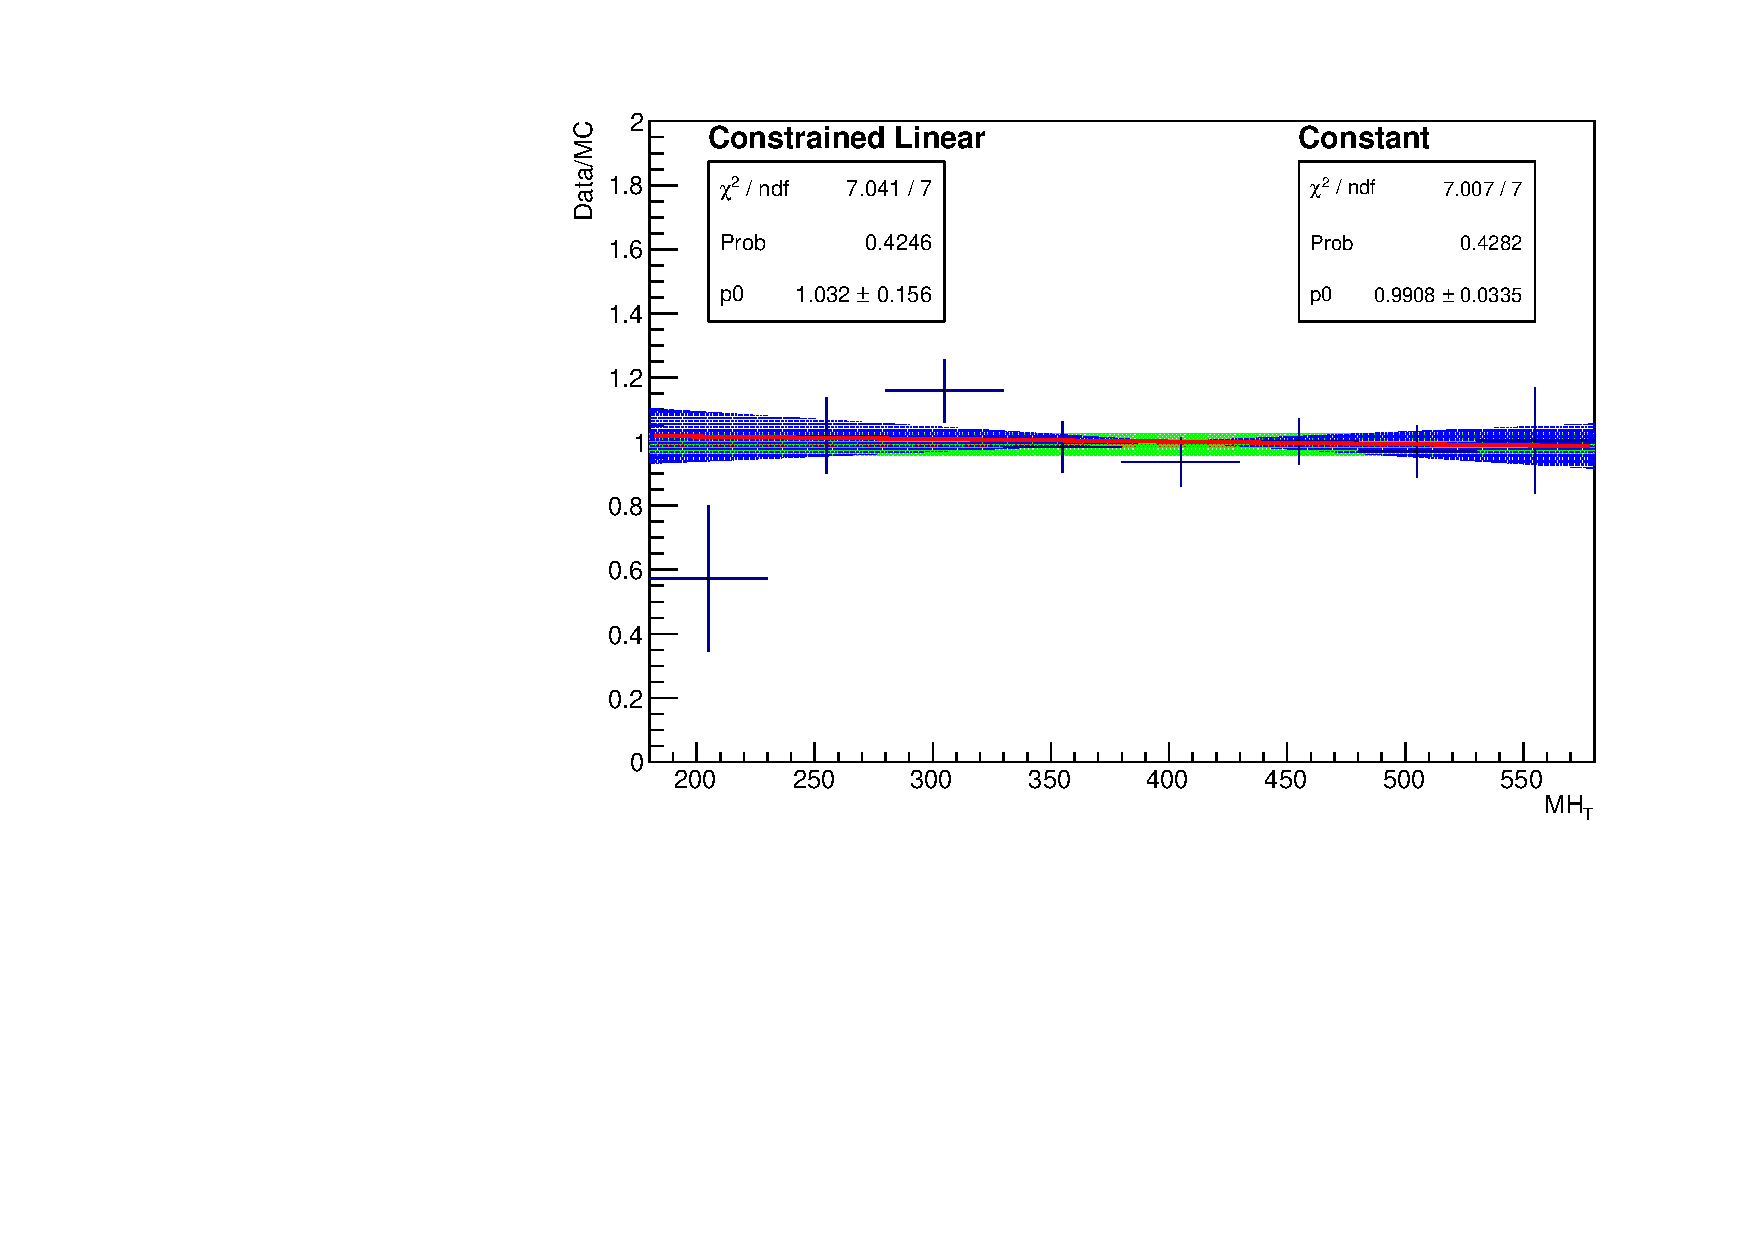
\includegraphics[width=0.5\textwidth]{figures/template/linear/mht_eq0b_le3j_ht_475_575_SinglePhoton.pdf}
  }~~
  \subfigure[\mmj]{
    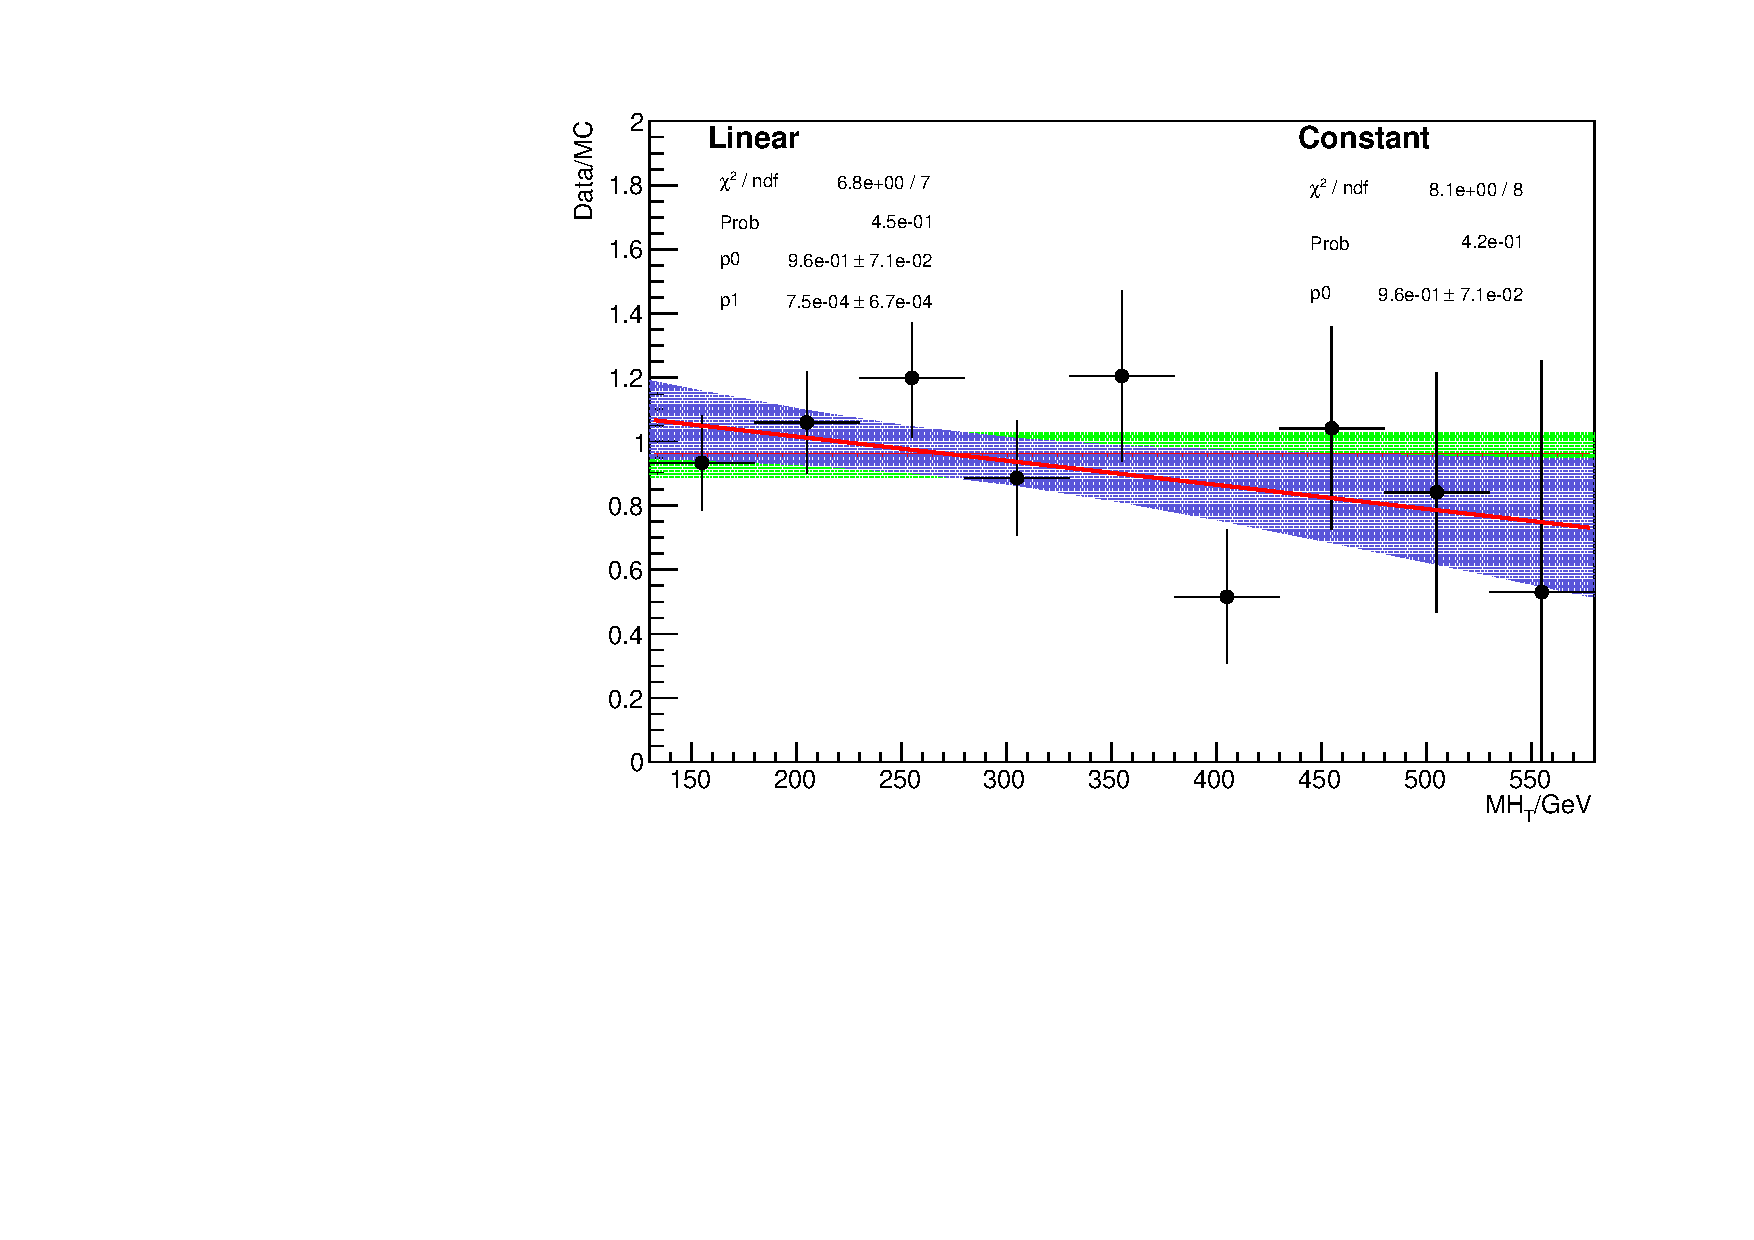
\includegraphics[width=0.5\textwidth]{figures/template/linear/mht_eq0b_le3j_ht_475_575_DoubleMu.pdf}
  }\\
  \subfigure[\mj]{
    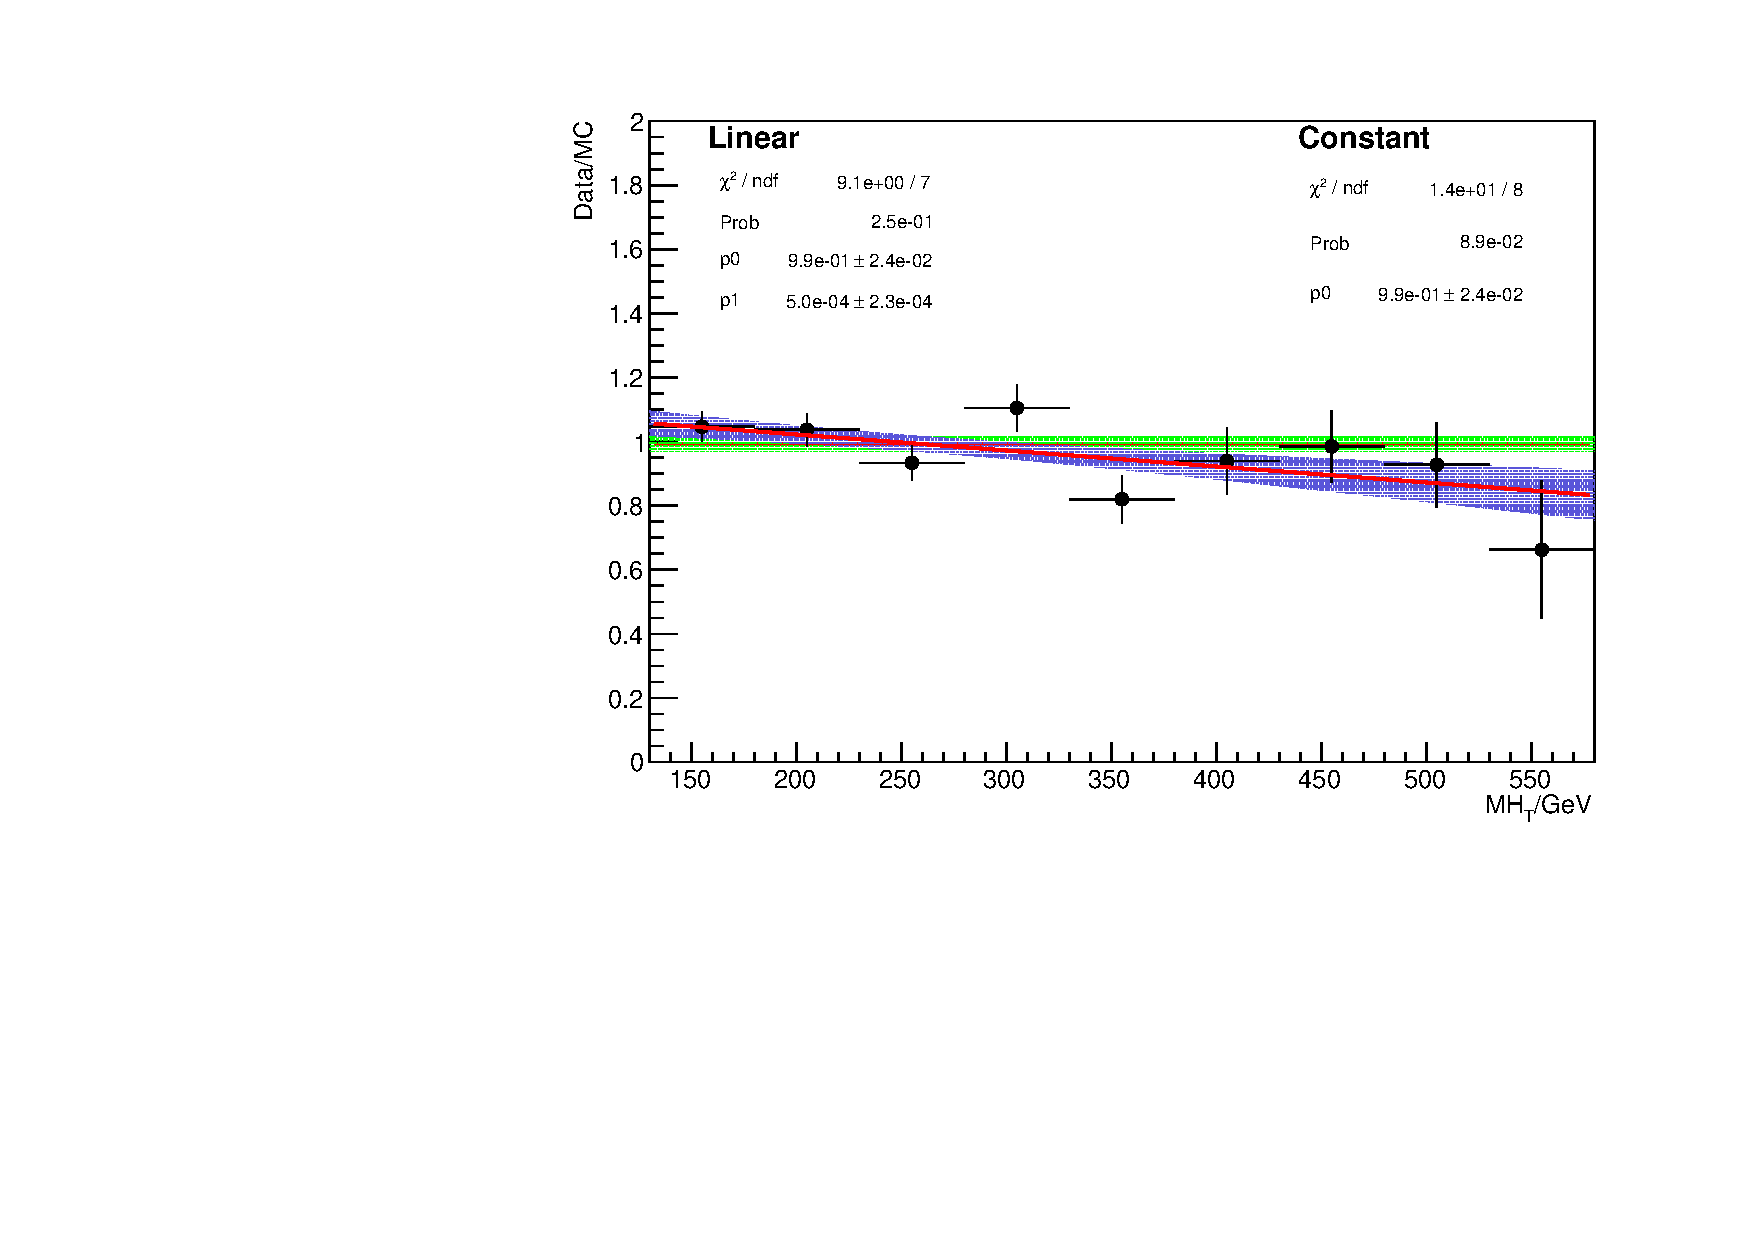
\includegraphics[width=0.5\textwidth]{figures/template/linear/mht_eq0b_le3j_ht_475_575_SingleMu.pdf}
  }~~
  \\
  \caption{\label{fig:linearFits0bLe3} 
  The data/MC distribution against \mht for the 0b, $\le3$j category and \scalht 475-575\GeV bin.
  The large bias in the linear component seen in Figure~\ref{fig:linearMotiv} is mitigated.}
\end{figure}

\begin{figure}[h!]
  \centering
  \subfigure[\gj]{
    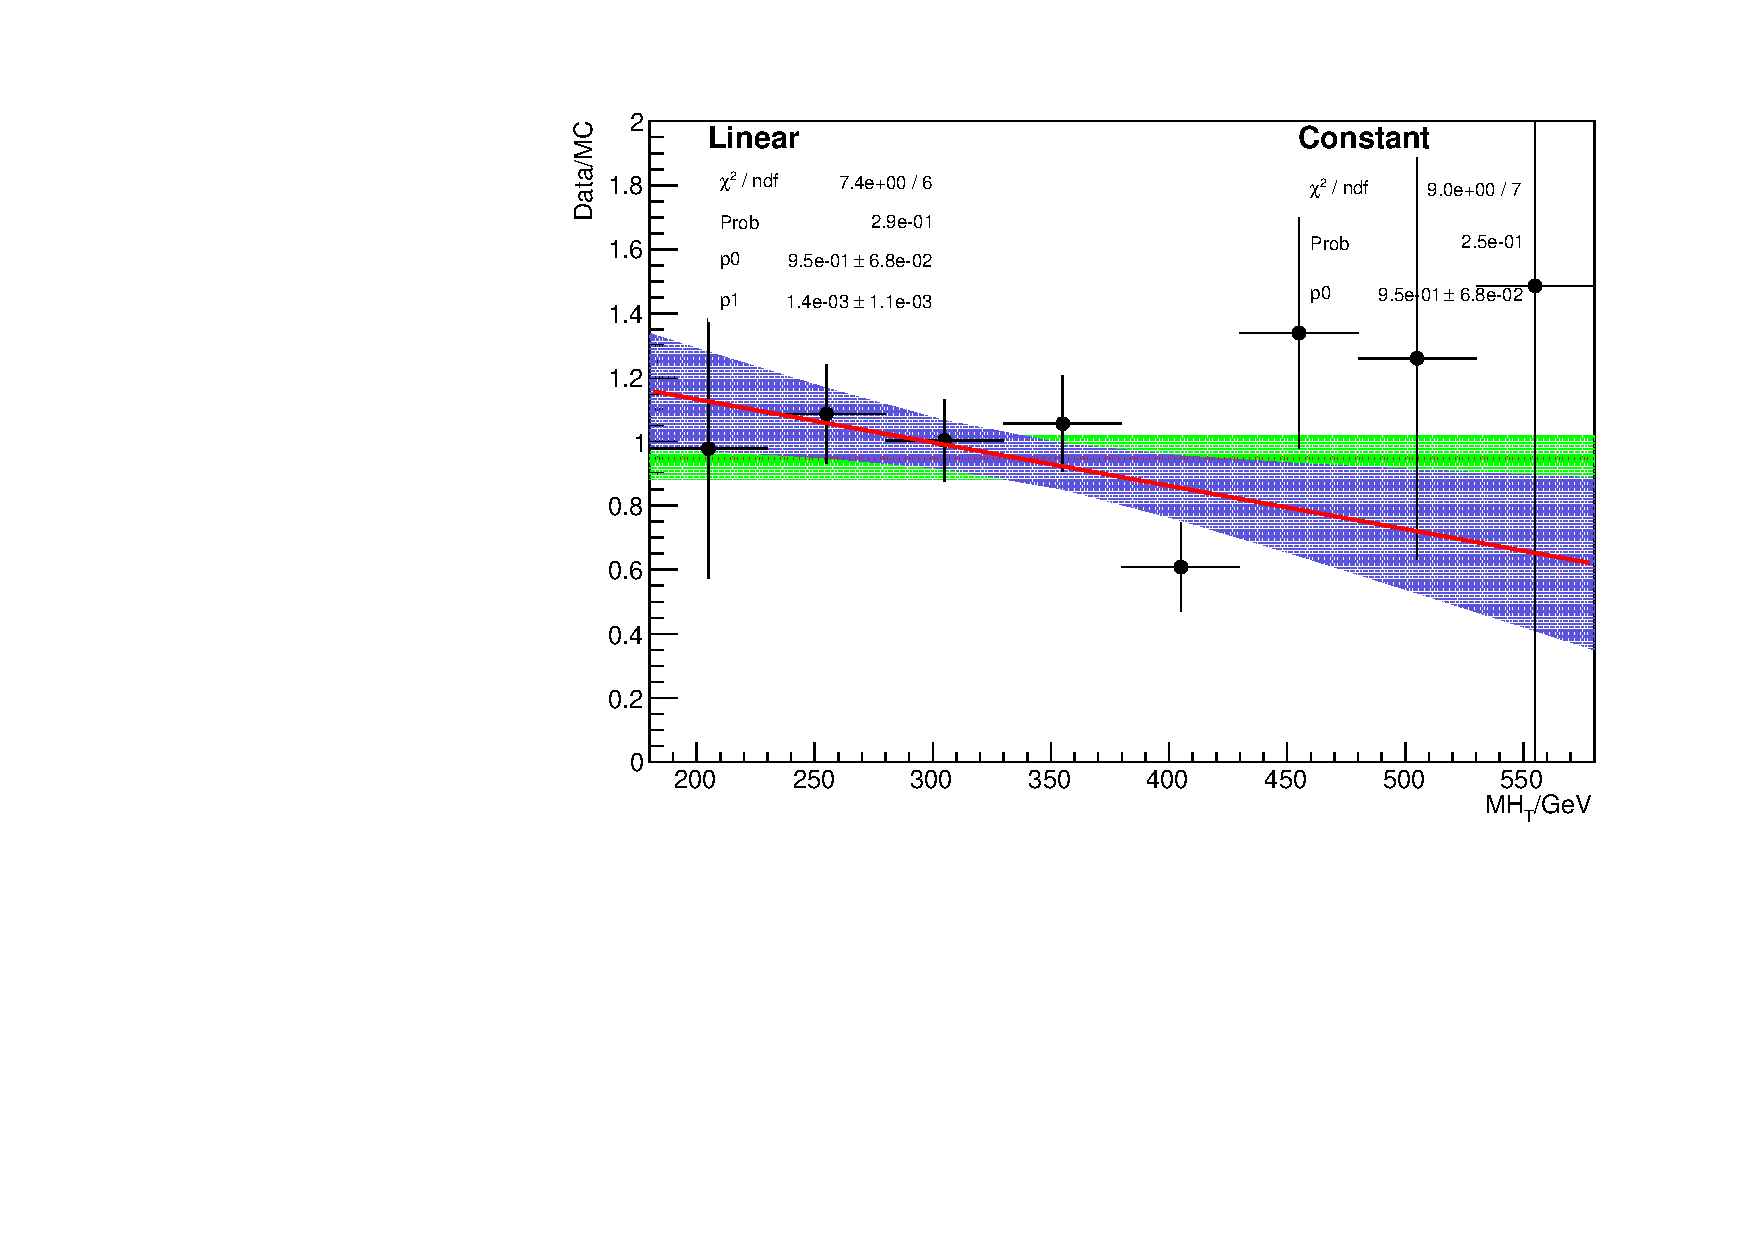
\includegraphics[width=0.5\textwidth]{figures/template/linear/mht_eq0b_ge4j_ht_475_575_SinglePhoton.pdf}
  }~~
  \subfigure[\mmj]{
    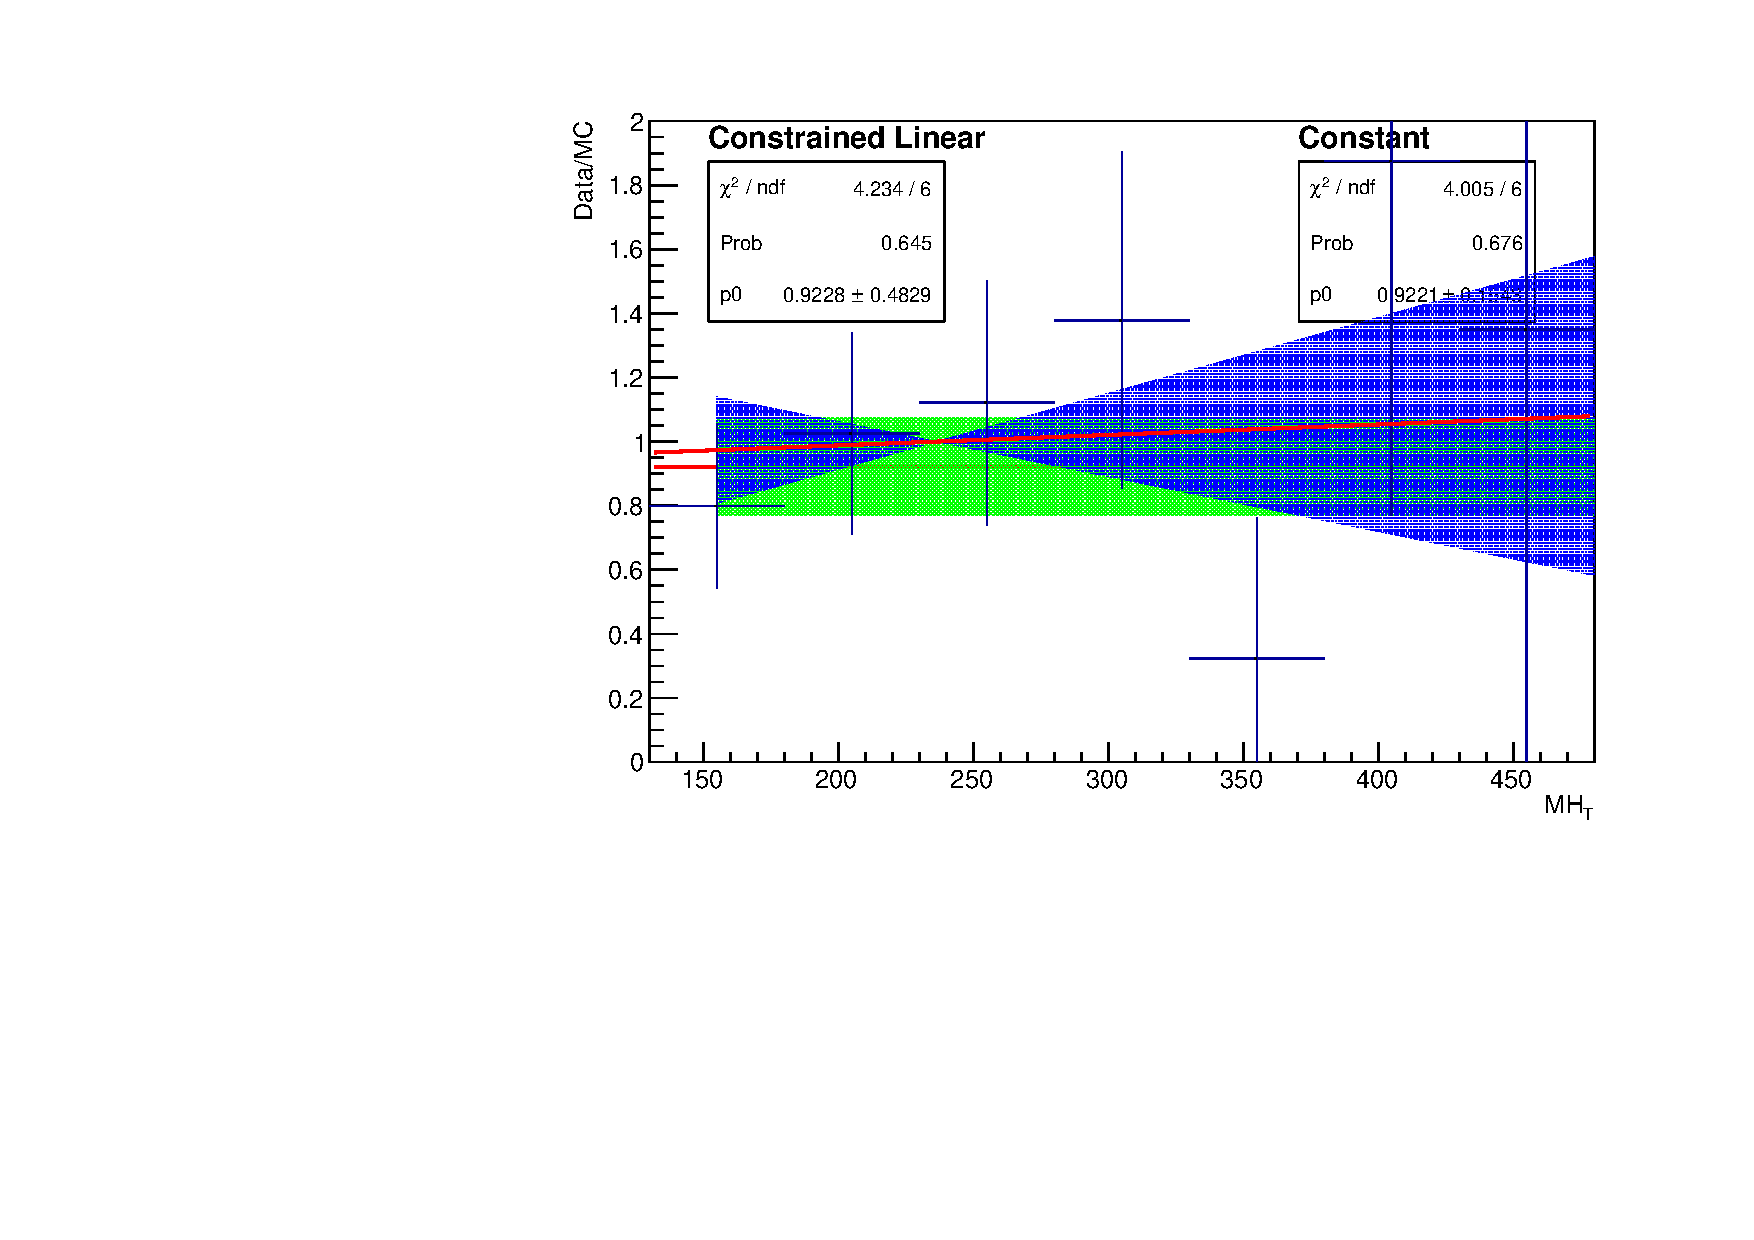
\includegraphics[width=0.5\textwidth]{figures/template/linear/mht_eq0b_ge4j_ht_475_575_DoubleMu.pdf}
  }\\
  \subfigure[\mj]{
    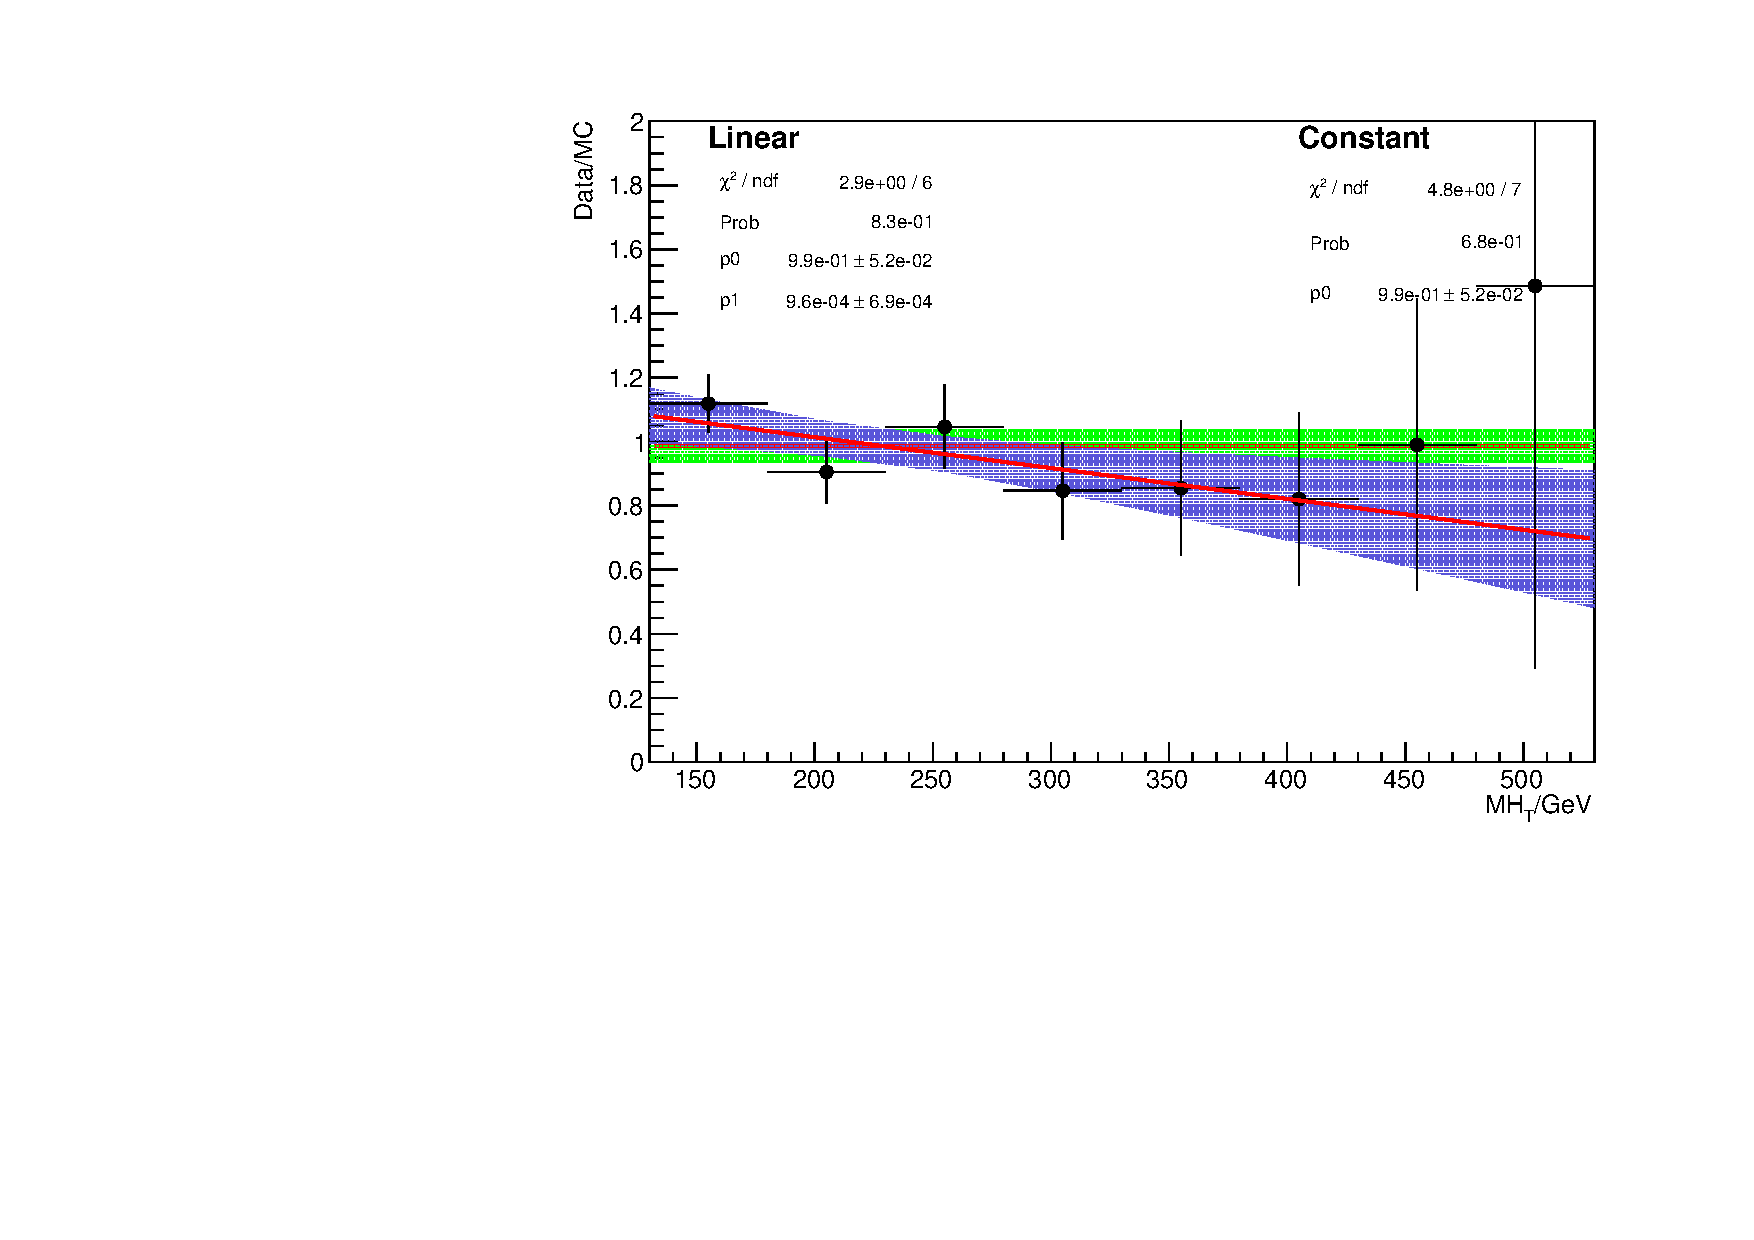
\includegraphics[width=0.5\textwidth]{figures/template/linear/mht_eq0b_ge4j_ht_475_575_SingleMu.pdf}
  }~~
  \\
  \caption{\label{fig:linearFits0bGe4} 
  The data/MC distribution against \mht for the 0b, $\ge4$j category and \scalht 475-575\GeV bin.
  The large bias in the linear component seen in Figure~\ref{fig:linearMotiv} is mitigated.}
\end{figure}

\begin{figure}[h!]
  \centering
  \subfigure[\gj]{
    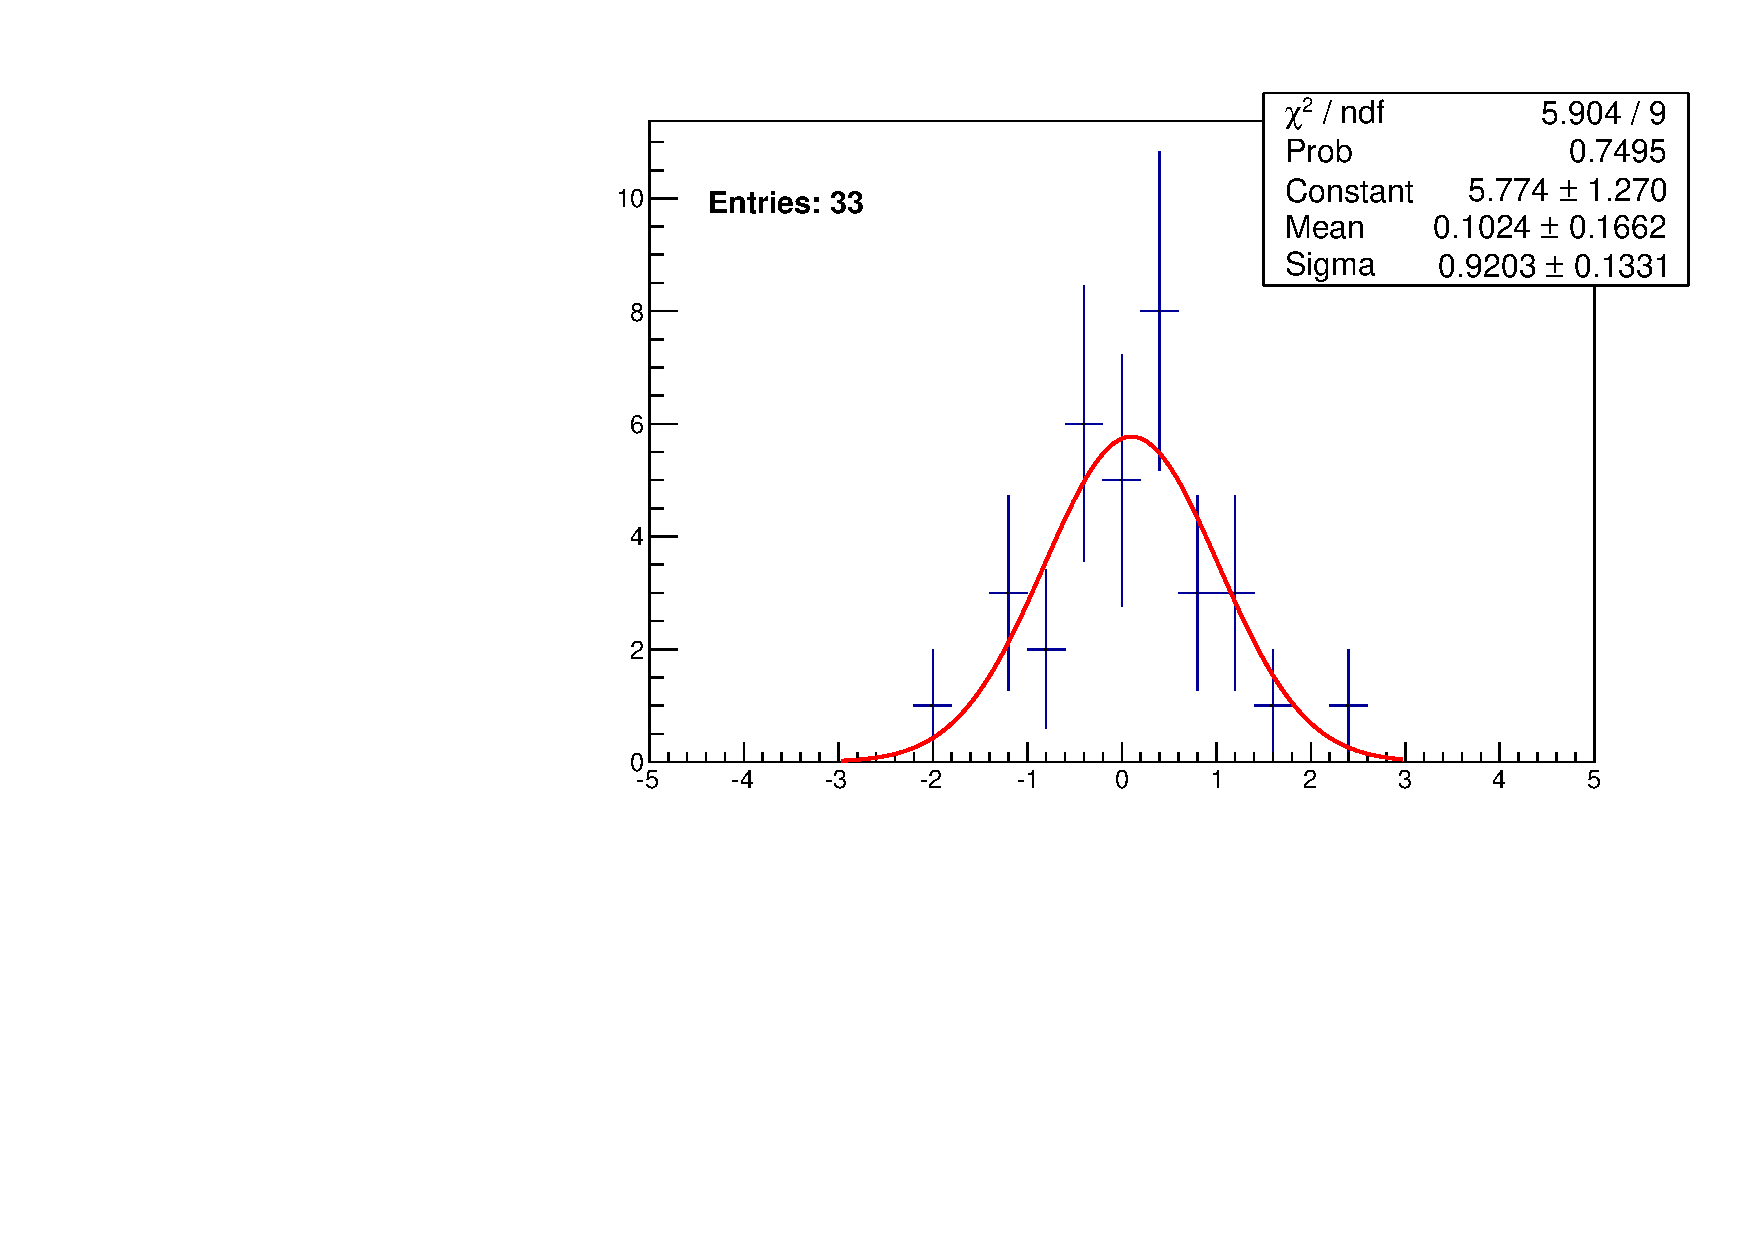
\includegraphics[width=0.5\textwidth]{figures/template/linear/pull_Linear2D_p1_SinglePhoton.pdf}
  }~~
  \subfigure[\mmj]{
    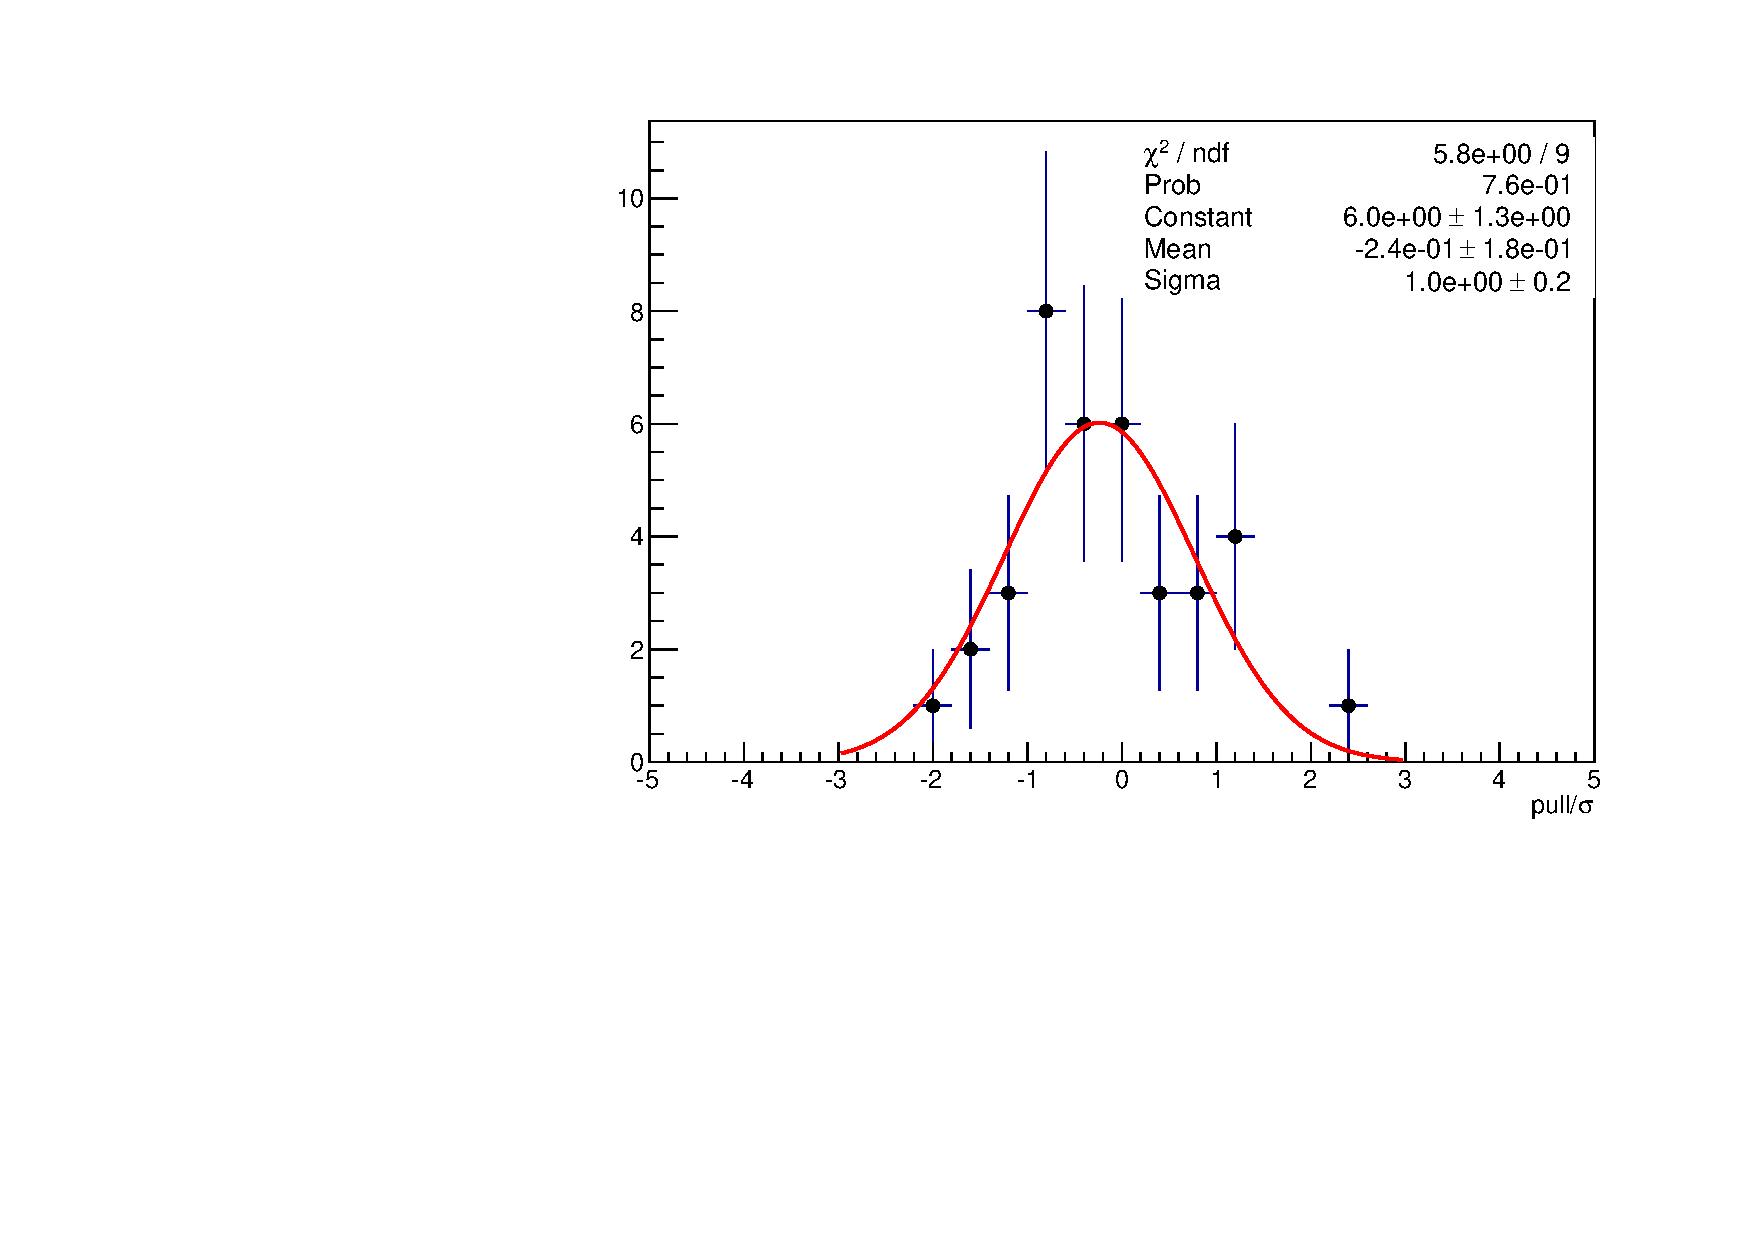
\includegraphics[width=0.5\textwidth]{figures/template/linear/pull_Linear2D_p1_DoubleMu.pdf}
  }\\
  \subfigure[\mj]{
    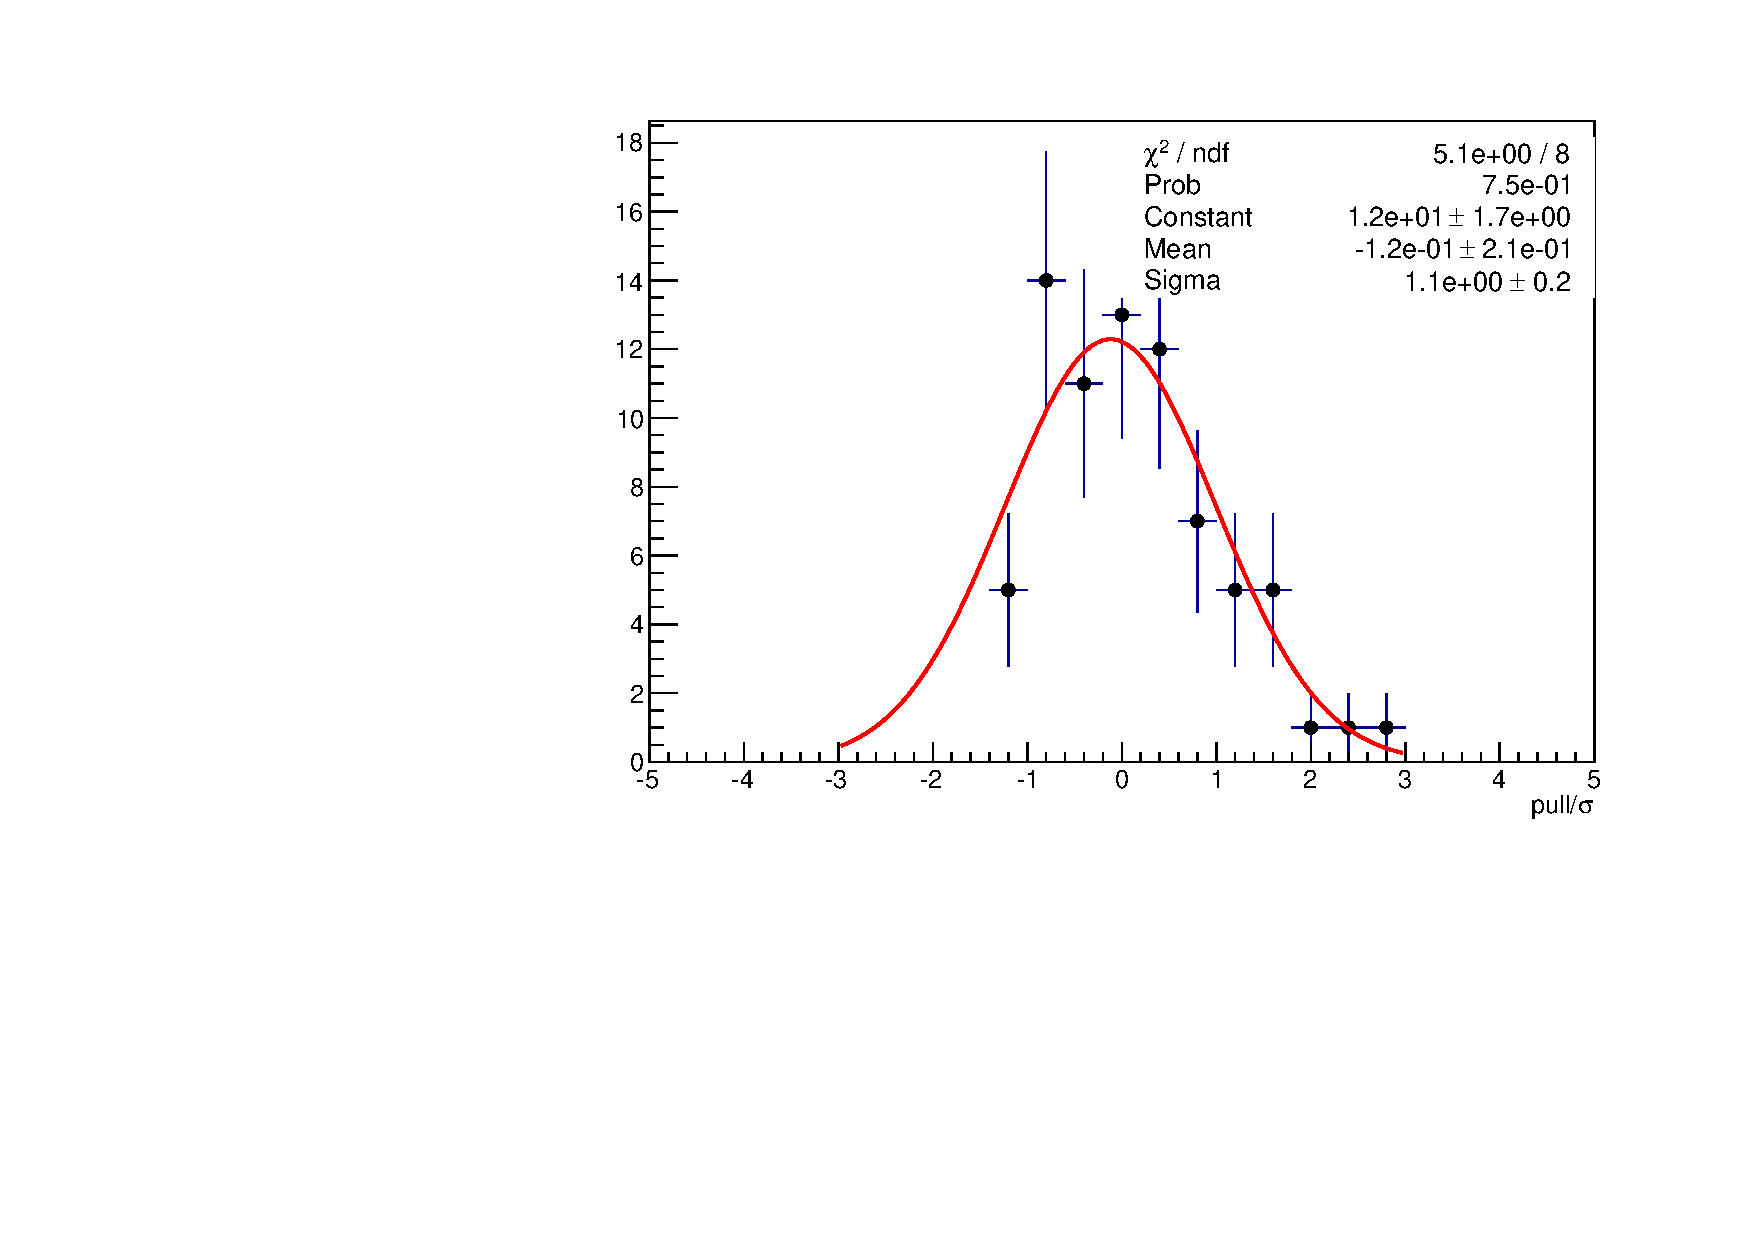
\includegraphics[width=0.5\textwidth]{figures/template/linear/pull_Linear2D_p1_SingleMu.pdf}
  }~~
  \\
  \caption{\label{fig:pulls} 
  The pull distribution of the linear parameter from the flat hypothesis showing no significant bias.}
\end{figure}
\begin{figure}[h!]
  \centering
  \subfigure[\gj]{
    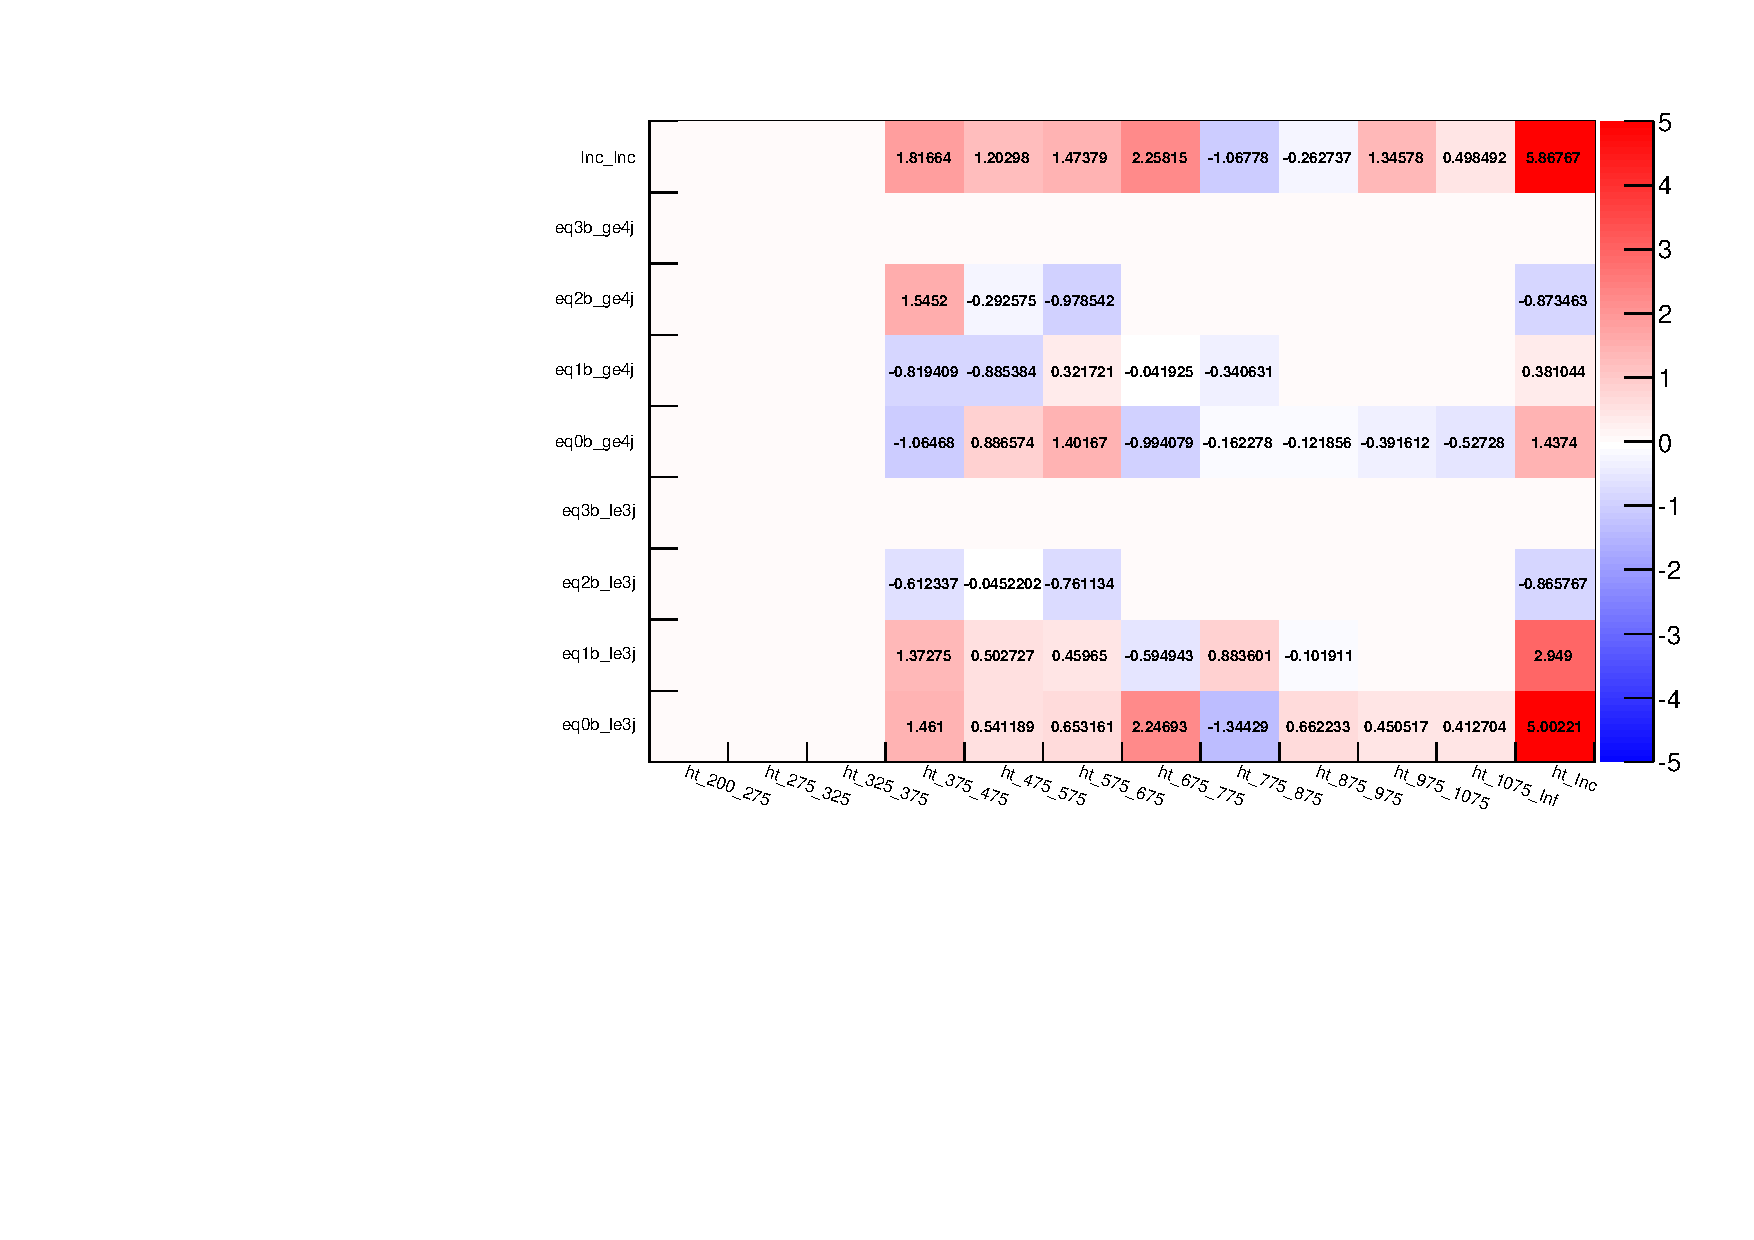
\includegraphics[width=0.5\textwidth]{figures/template/linear/frenchFlagPull_Linear2D_p1_SinglePhoton.pdf}
  }~~
  \subfigure[\mmj]{
    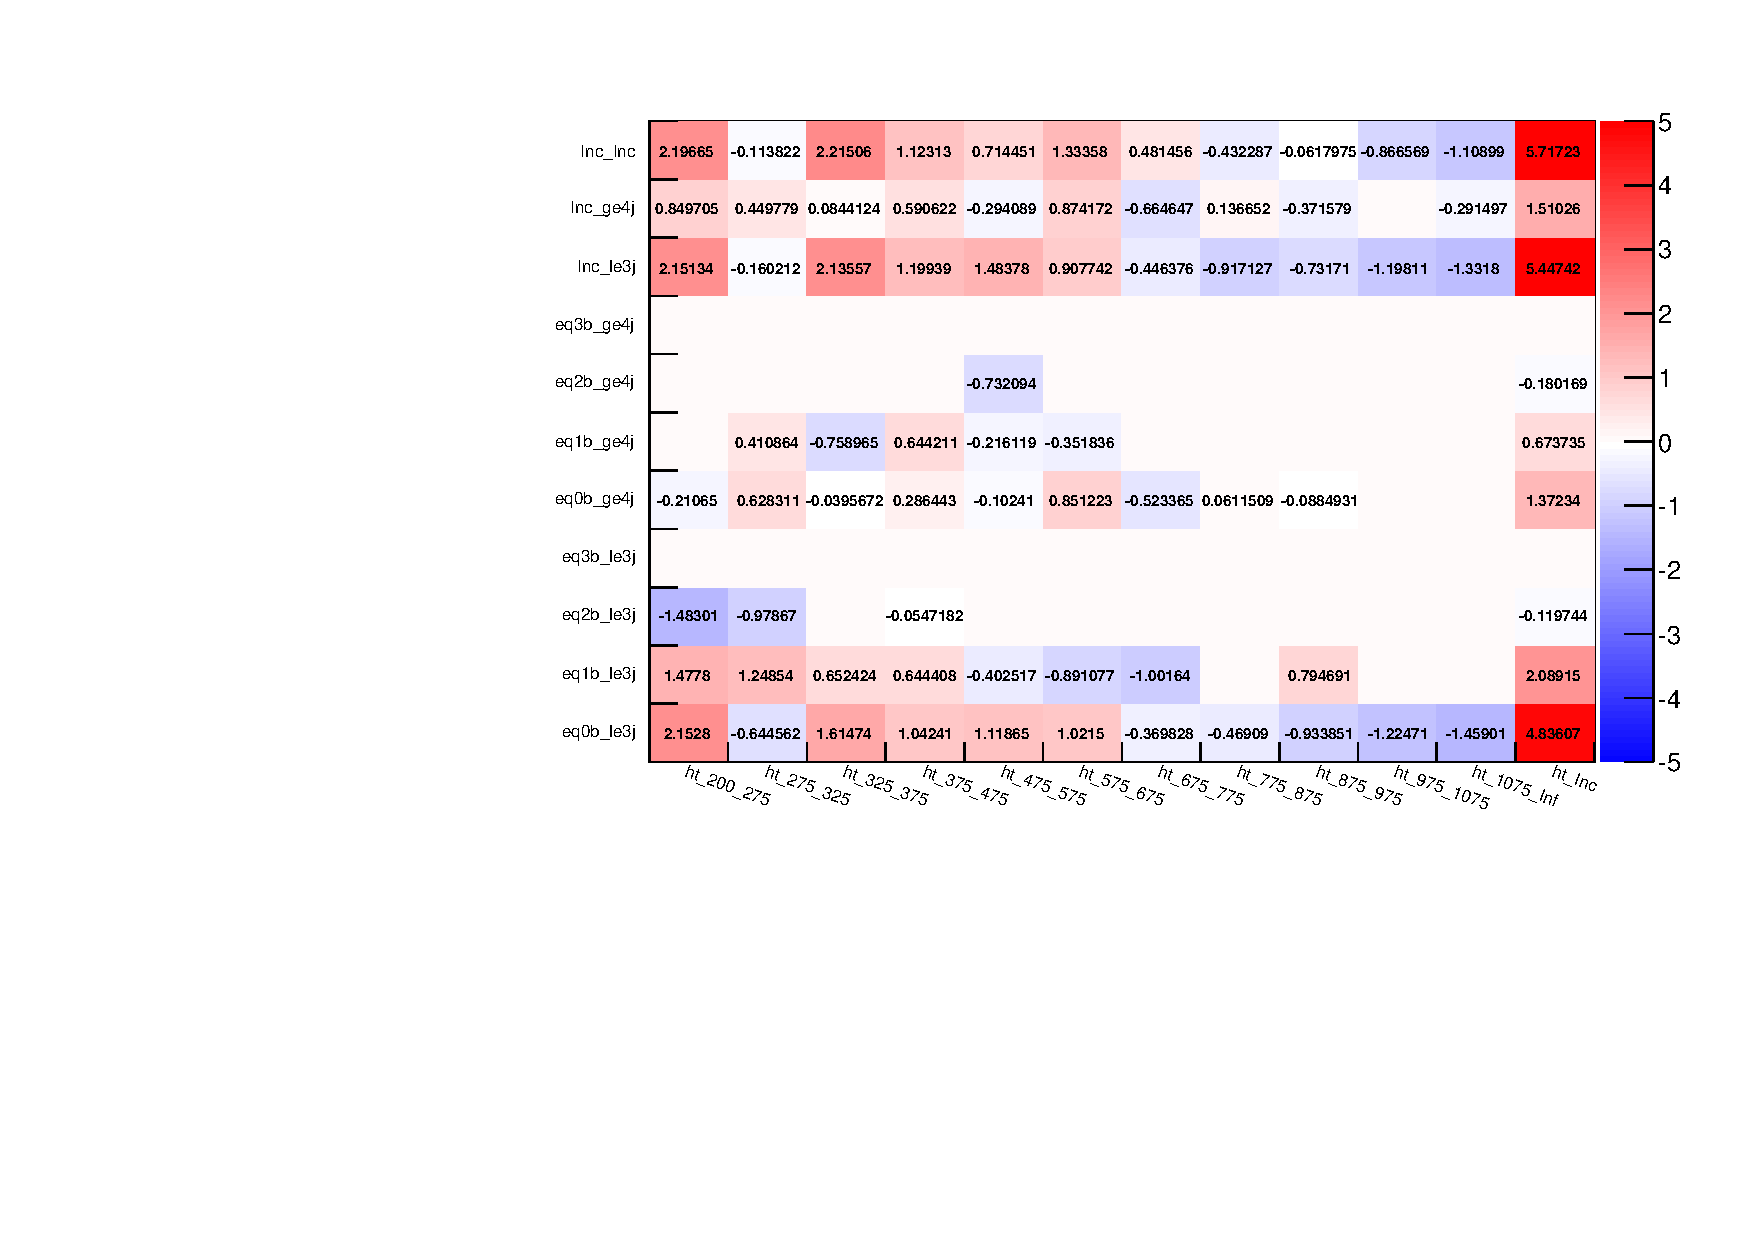
\includegraphics[width=0.5\textwidth]{figures/template/linear/frenchFlagPull_Linear2D_p1_DoubleMu.pdf}
  }\\
  \subfigure[\mj]{
    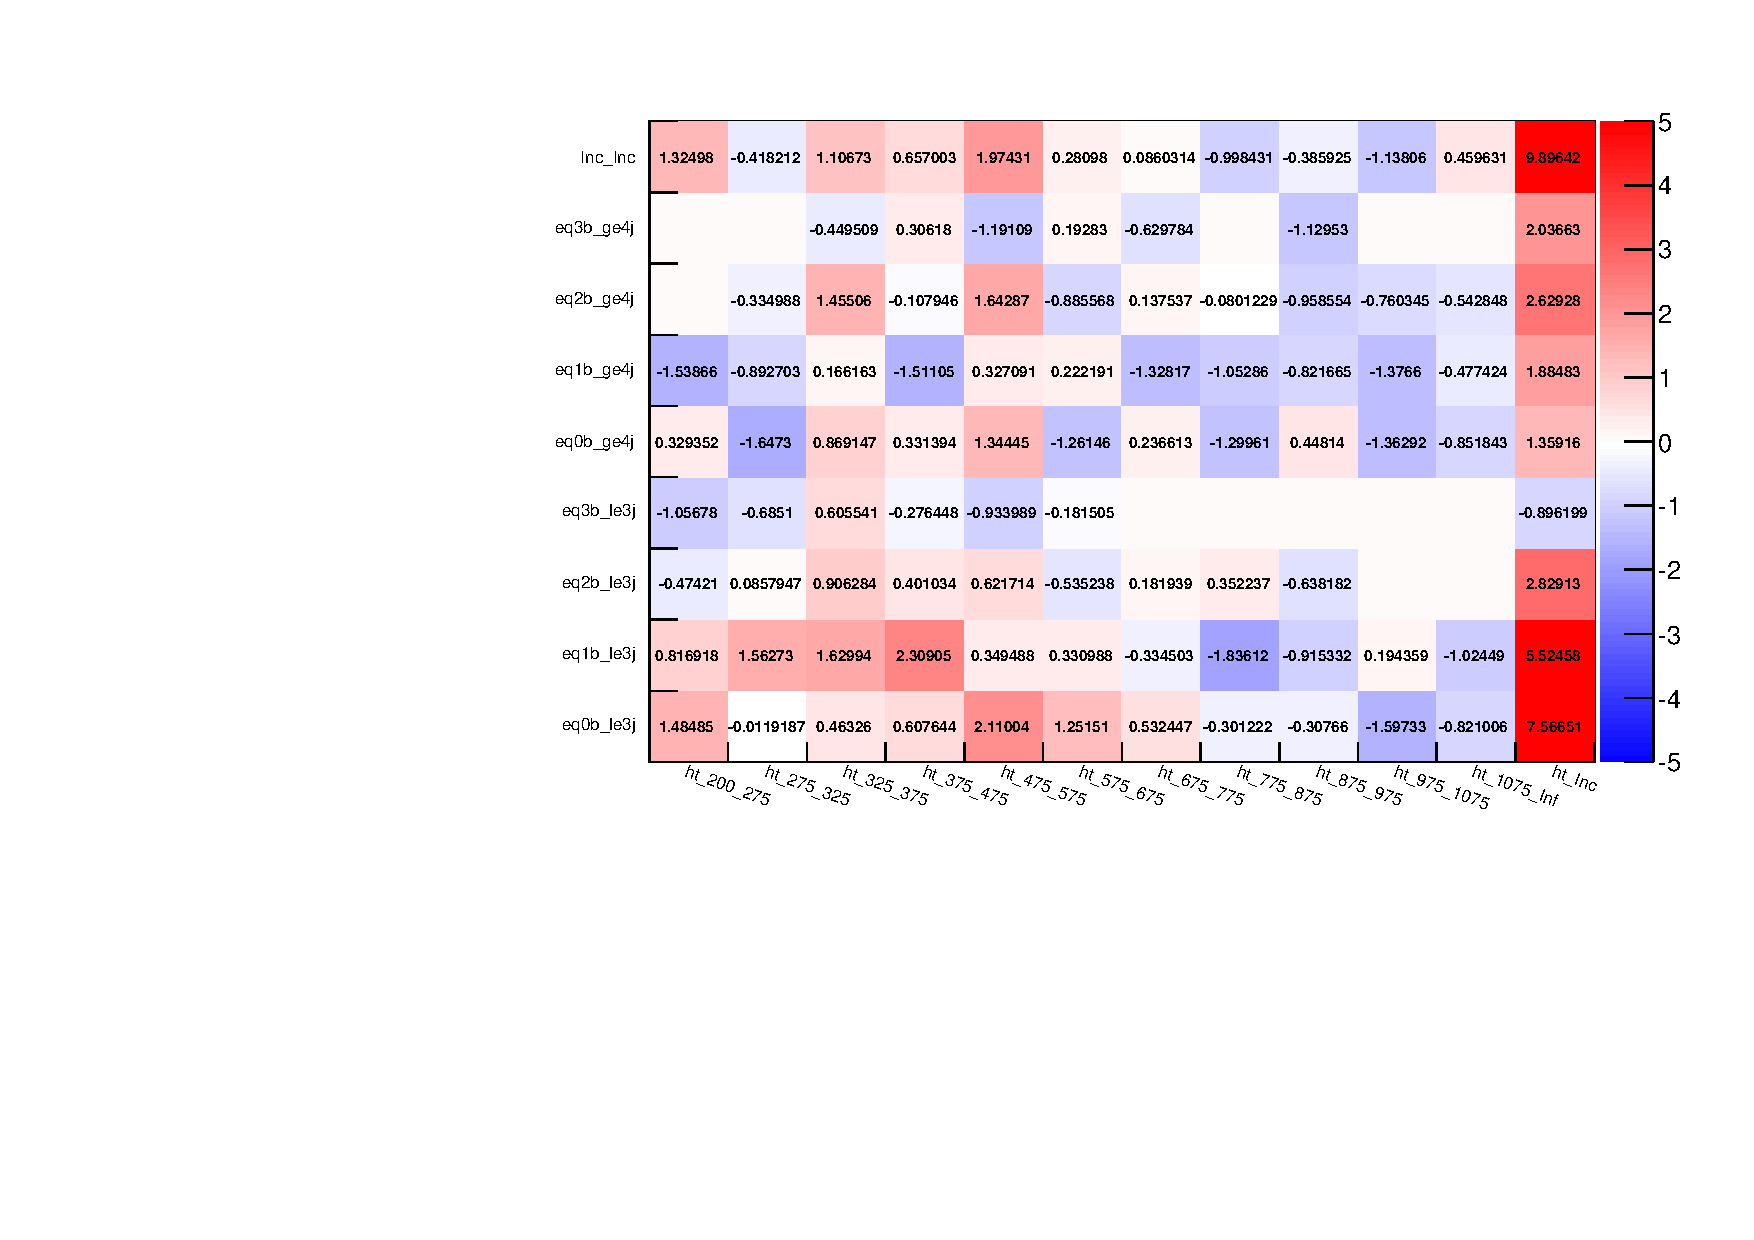
\includegraphics[width=0.5\textwidth]{figures/template/linear/frenchFlagPull_Linear2D_p1_SingleMu.pdf}
  }~~
  \\
  \caption{\label{fig:frenchFlagPulls} The pull distribution of the linear parameter from the flat hypothesis across all
  \scalht bins and categories. There are no significant pulls for the \scalht binned
  fits while the \scalht inclusive case shows very large pulls as expected. 
  Due to trigger requirements the \gj control sample may only be used for \scalht $> 375$\GeV.}
\end{figure}

\begin{figure}[h!]
  \centering
    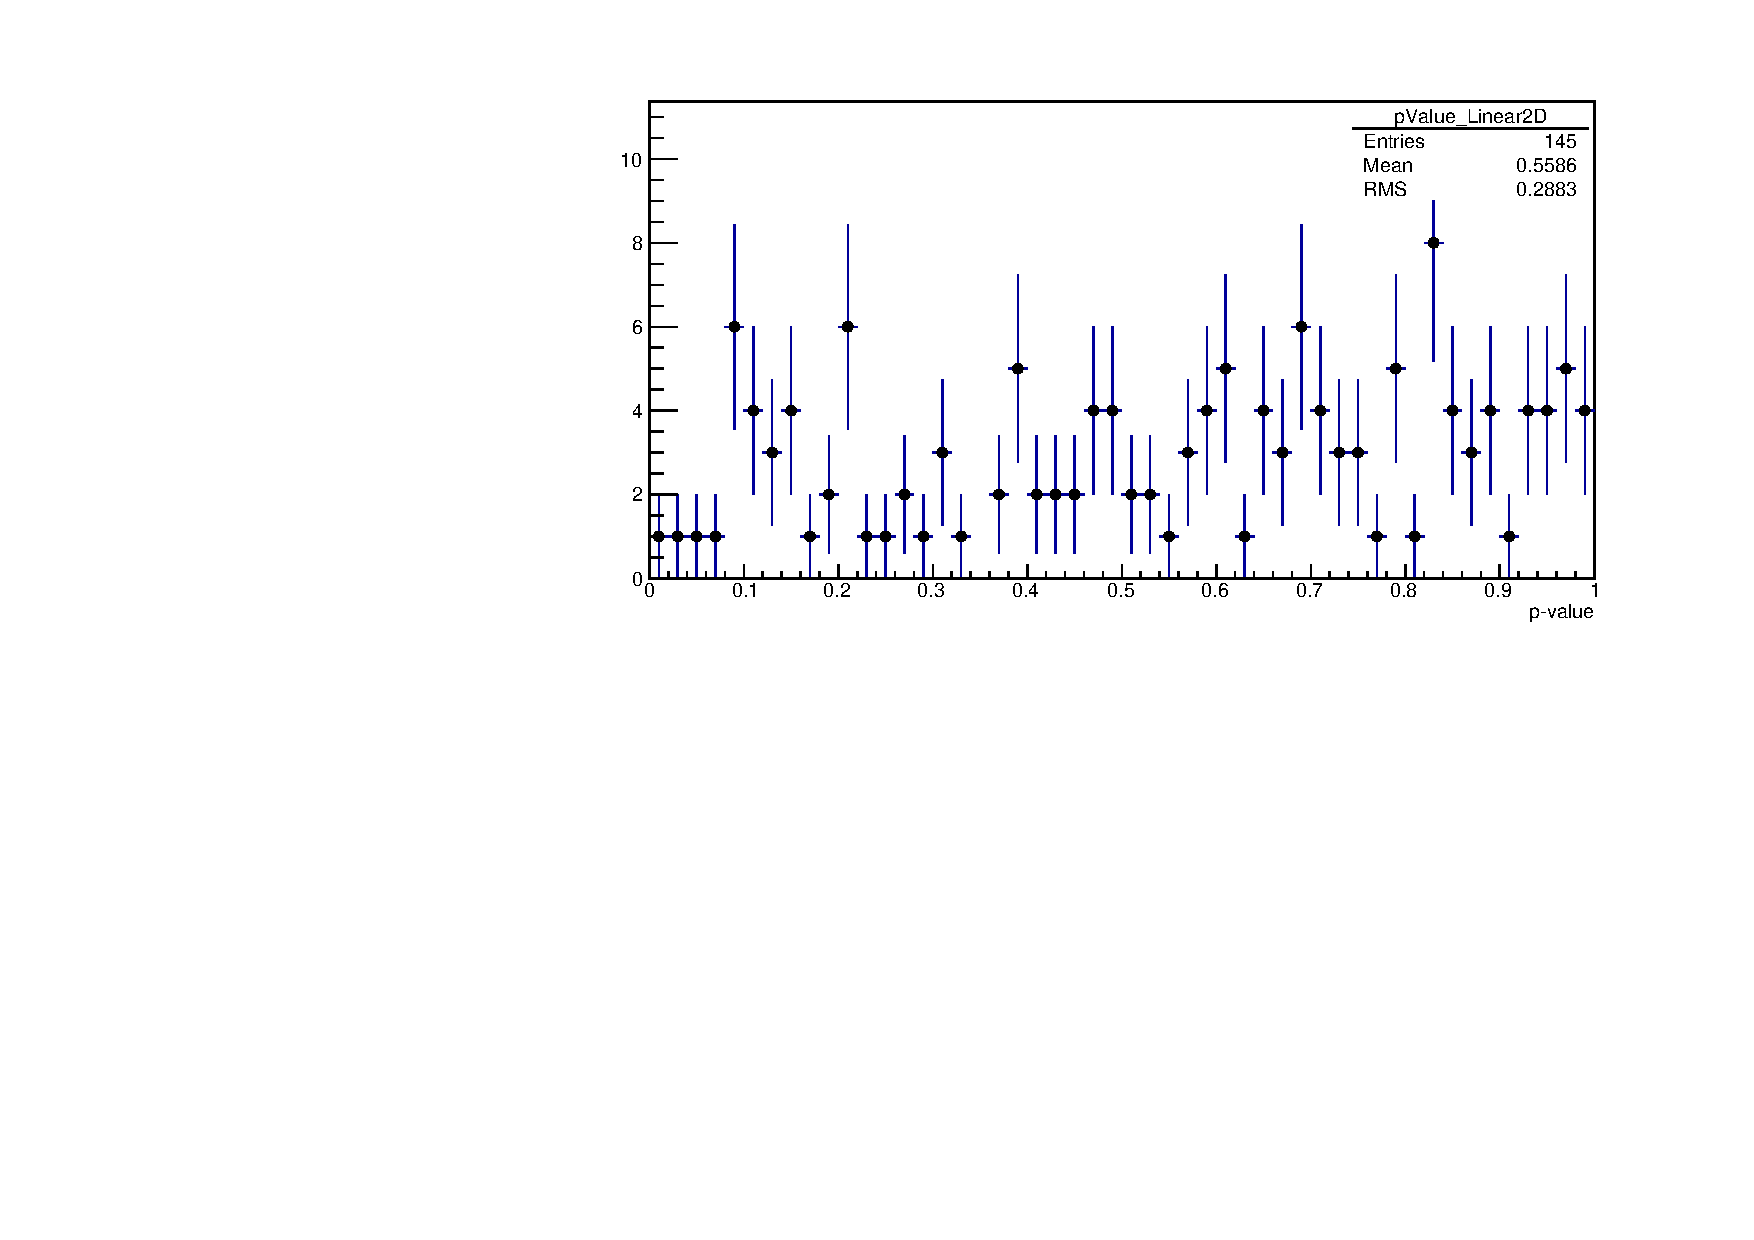
\includegraphics[width=0.8\textwidth]{figures/template/linear/pValueAll.pdf}
  \\
  \caption{\label{fig:pValues} The distributions of the p-value for the linear fit.} 
\end{figure}
\subsection{Deriving systematics on the \texorpdfstring{\mht} dimension}
\label{sec:systMhtDimension}
The systematic in the \mht dimension is extracted from the hypothesis
of no bias. This is done by using the control regions 
to determine the statistical precision to which this hypothesis can
be confirmed. This information is then used to derive the systematic 
uncertainty, as described in the following. 

Each background in the signal region (\ttbar/W  and \zInv~) is predicted 
using several control regions. In order to determine the uncertainty in
the \mht dimension a combined linear fit is made over all relevant control regions
of the linear function. A requirement of at least 10 events and a non-trivial
number of degrees of freedom is made to ensure a reasonable fit. Where this
requiement is not satisfied the \mht distribution is not used in the signal region.
The uncertainty on the linear parameter from the fit is then
used to define the up and down one sigma variations of the nominal template.
As a conservative estimate, the best fit value of the parameter is 
added in quadrature to its uncertainty in order to derive the overall variation.

The result of this procedure is shown in Figure~\ref{fig:signalOverlay} for different 
\scalht bins and categories, using the data from the 8 \TeV signal region. 
Here the template variations for both relevant backgrounds are combined to show 
the overall uncertainty on the \mht dimension. The scatter of the points around 
one is compatible with statistical fluctuations
as no signal has been observed in this data sample.

An additional validation is carried out by comparing expected and observed uncertainties
on the linear parameter defining the template variations.
The expected errors are derived by using a linear fit to the MC/MC ratio where the numerator
have errors given by the Poisson uncertainty on the number of predicted counts while
the uncertainty on the denominator comes from the statistical uncertainty on the
MC prediction. The relative errors on $1+p_1$ derived from this approach 
for \ttbar/W and \zInv~ are shown in Figure~\ref{fig:expectedObservedTtw} 
and Figure~\ref{fig:expectedObservedZinv} and compared to those observed.
These show good agreement which provides additional motivation for the 
zero bias hypothesis as well as validating the method for deriving expected uncertainties.


\begin{figure}[h!]
  \centering
  \subfigure[Category 0b, $\le3$j and $\scalht$ $375-475$ \GeV]{
    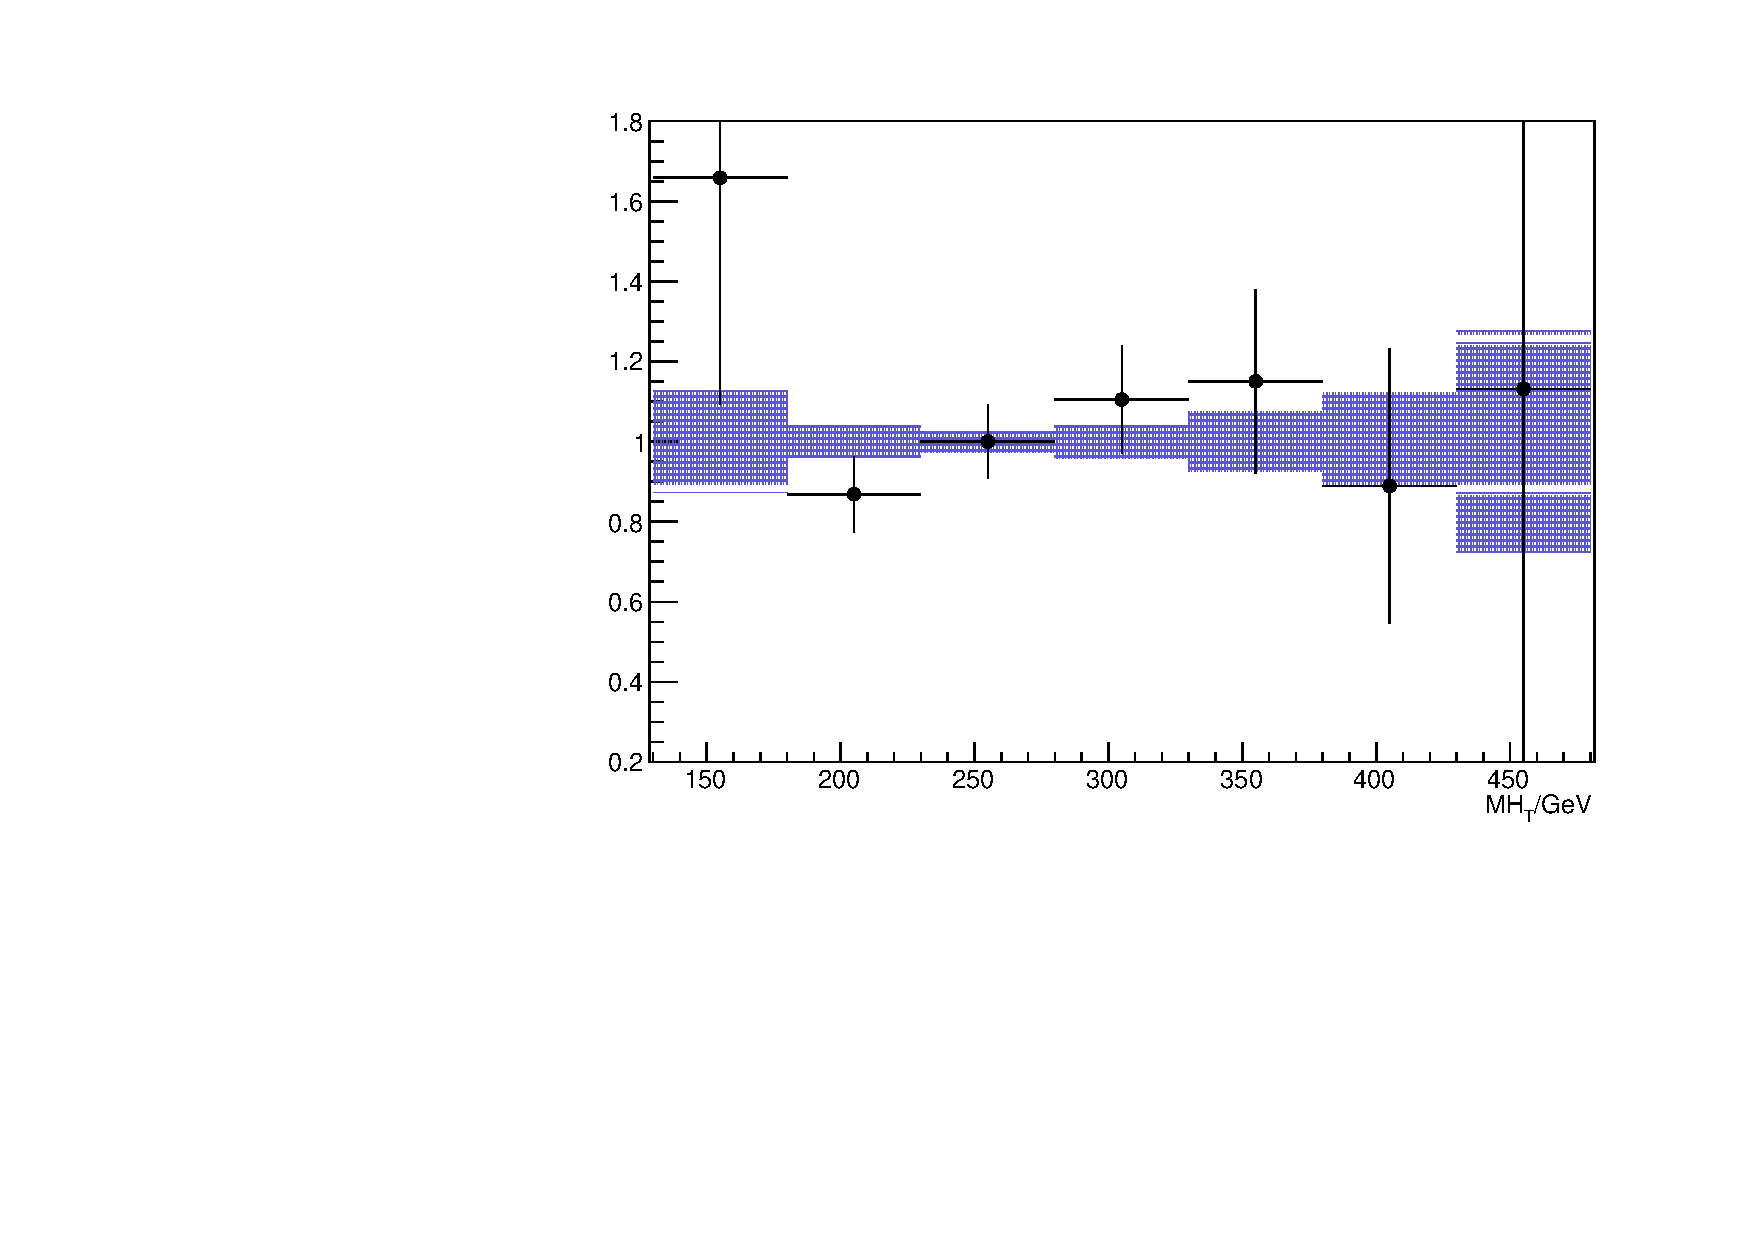
\includegraphics[width=0.5\textwidth]{figures/template/linear/mht_eq0b_ge4j_ht_375_475_signalOverlay.pdf}
  }~~
  \subfigure[Category 1b, $\le3$j and $\scalht$ $375-475$ \GeV]{
    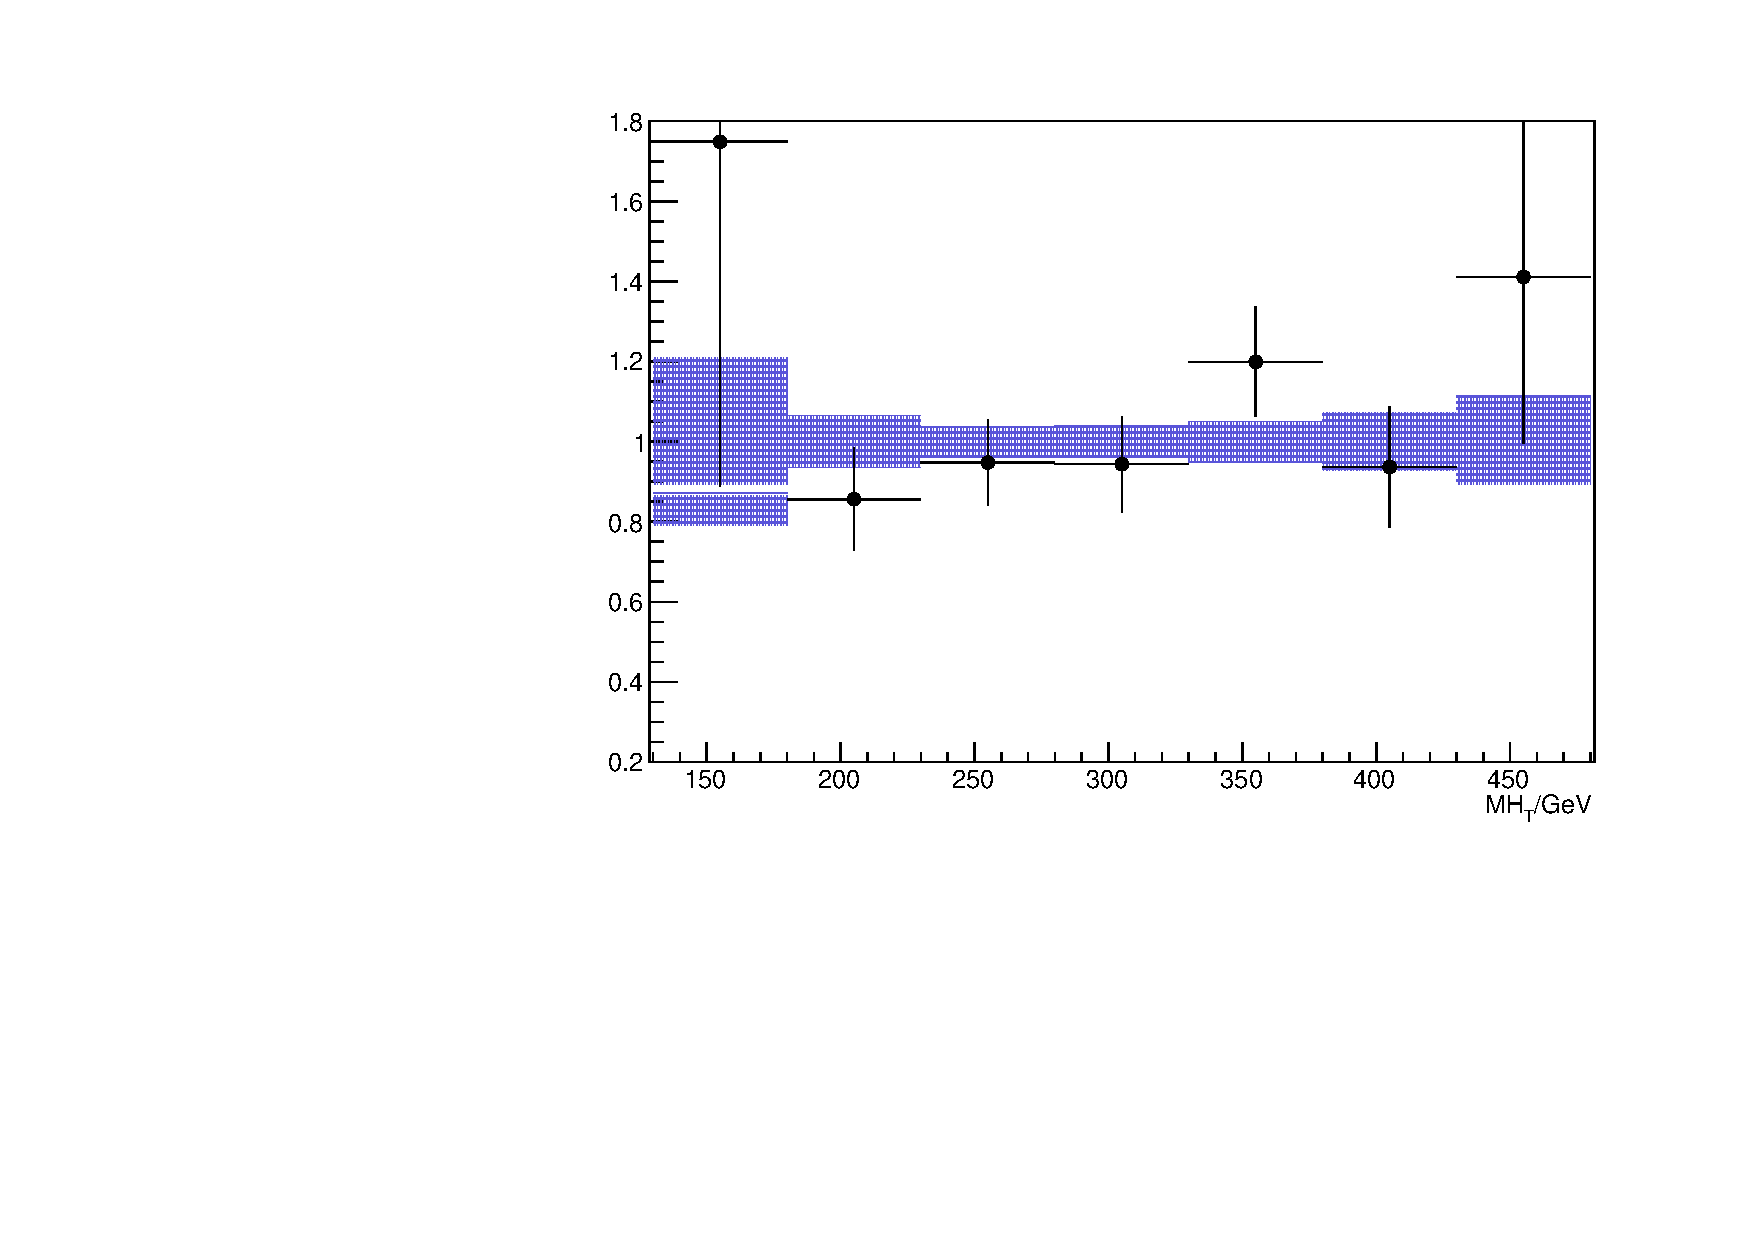
\includegraphics[width=0.5\textwidth]{figures/template/linear/mht_eq1b_le3j_ht_375_475_signalOverlay.pdf}
  }\\
  \subfigure[Category 0b, $\ge4$j and $\scalht$ $375-475$ \GeV]{
    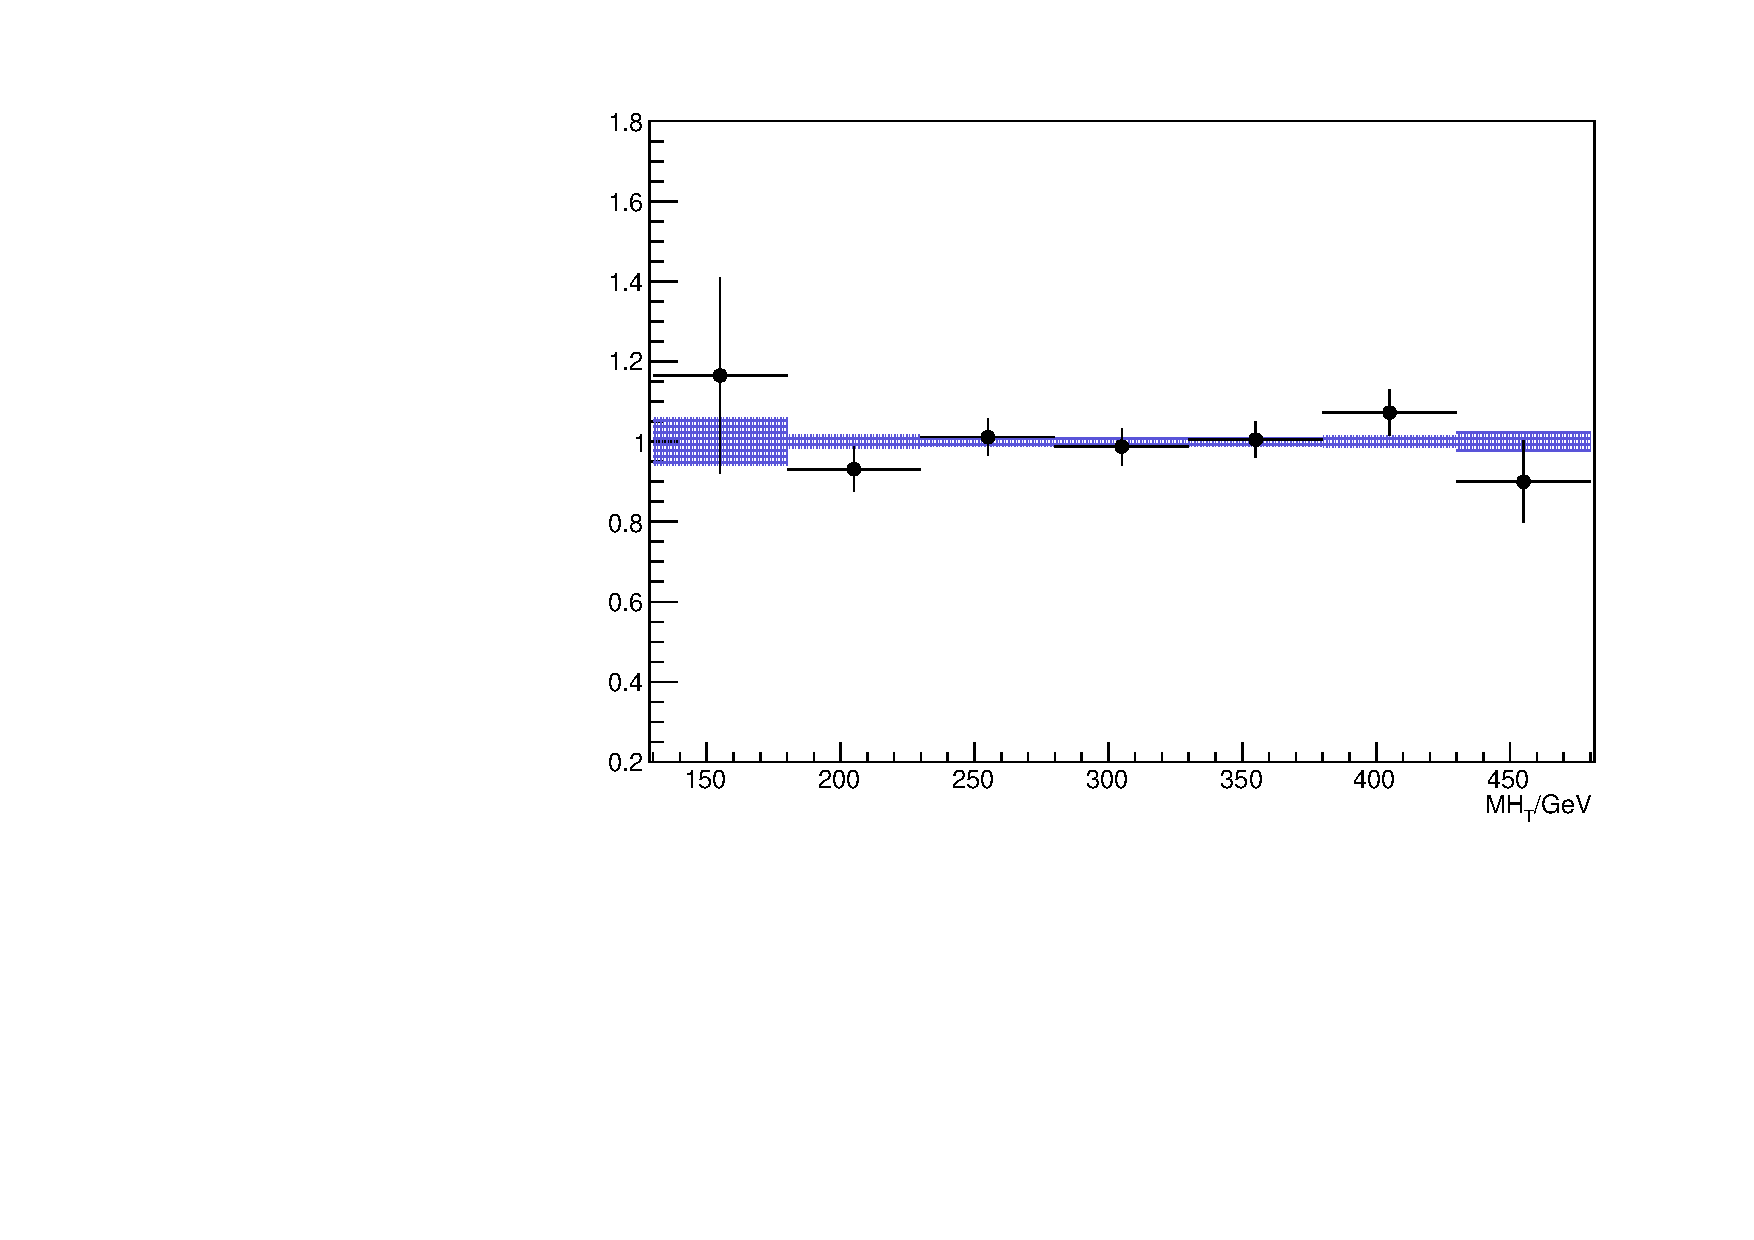
\includegraphics[width=0.5\textwidth]{figures/template/linear/mht_eq0b_le3j_ht_375_475_signalOverlay.pdf}
  }~~
  \subfigure[Category 0b, $\le3$j and $\scalht$ $475-575$ \GeV]{
    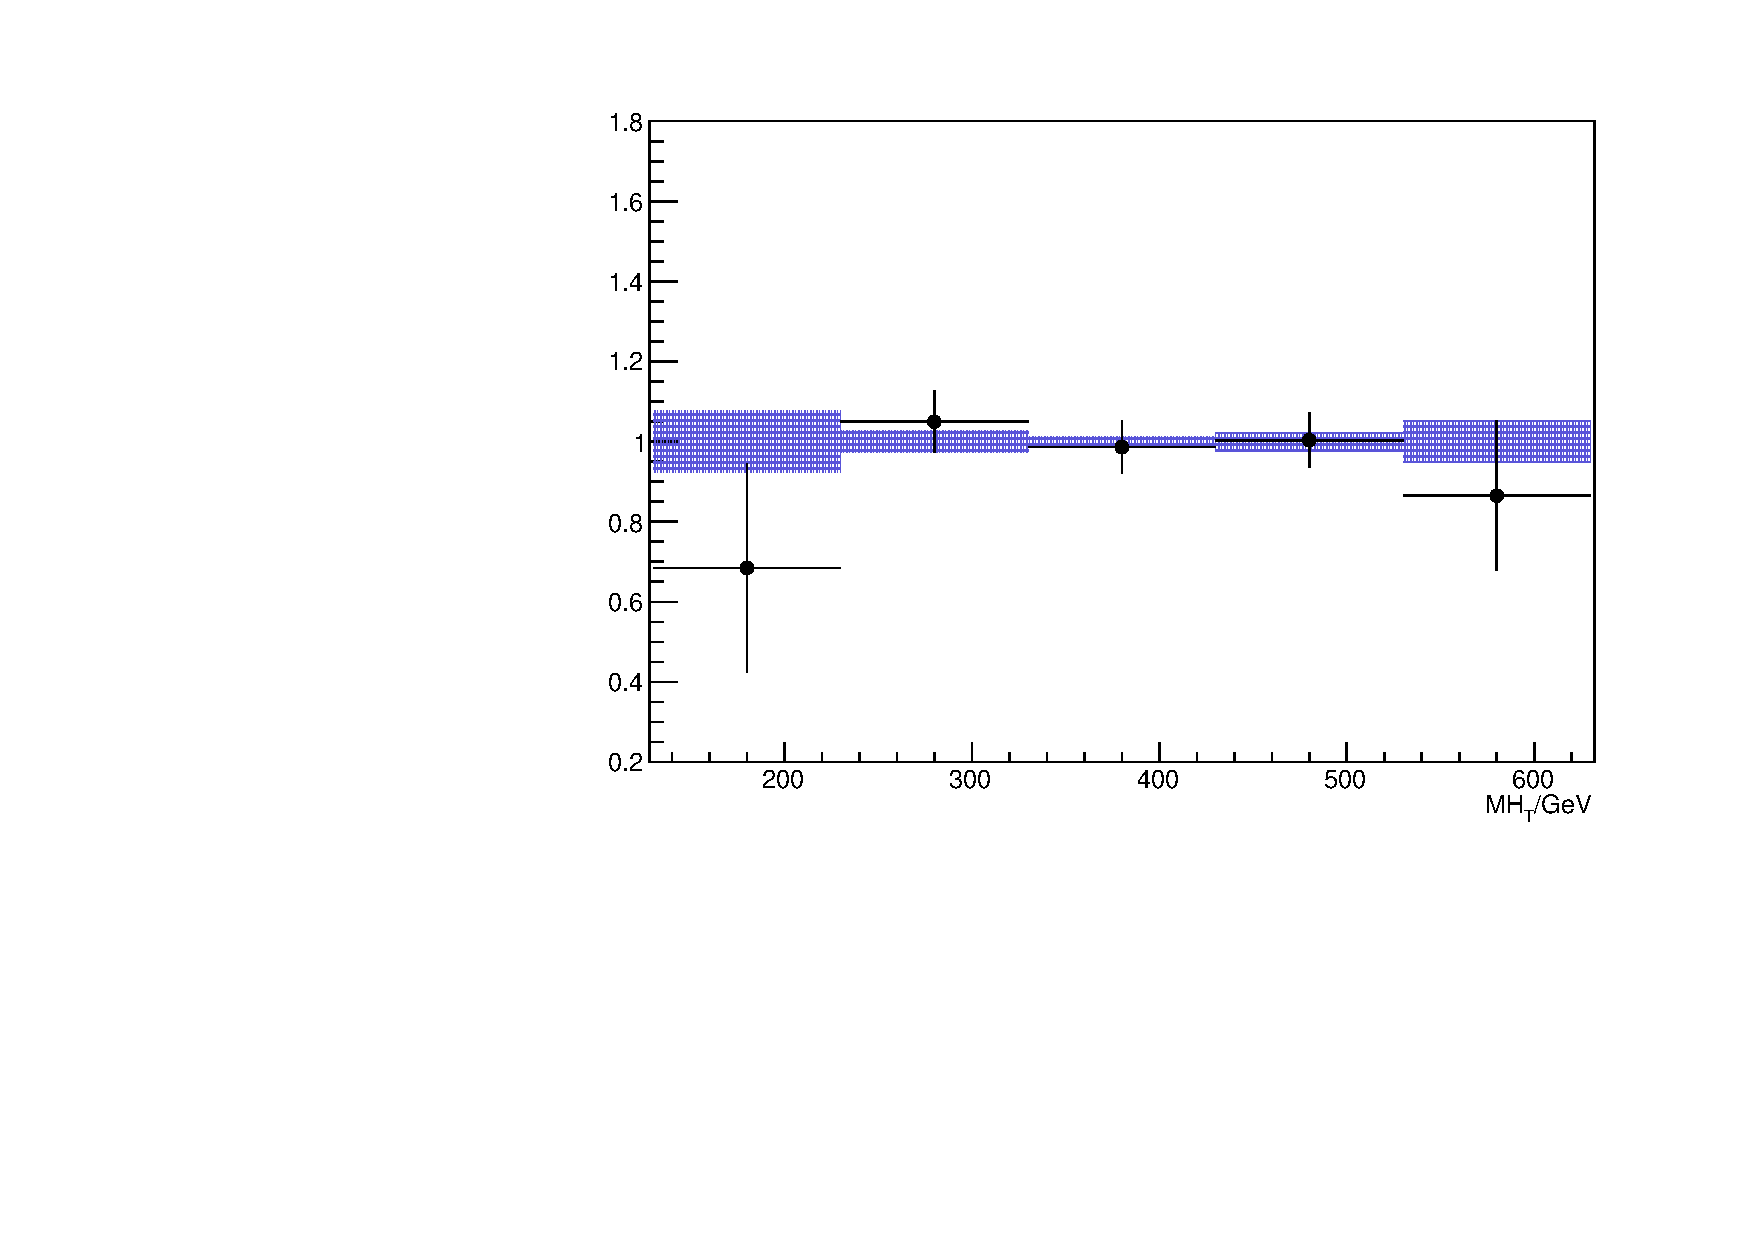
\includegraphics[width=0.5\textwidth]{figures/template/linear/mht_eq0b_le3j_ht_475_575_signalOverlay.pdf}
  }~~
  \\
  \caption{\label{fig:signalOverlay} Signal data/MC shown with template variations predicted from 
  the control regions.}
\end{figure}

\begin{figure}[h!]
  \centering
  \subfigure[\label{fig:expectedTtw} Expected uncertainties]{
    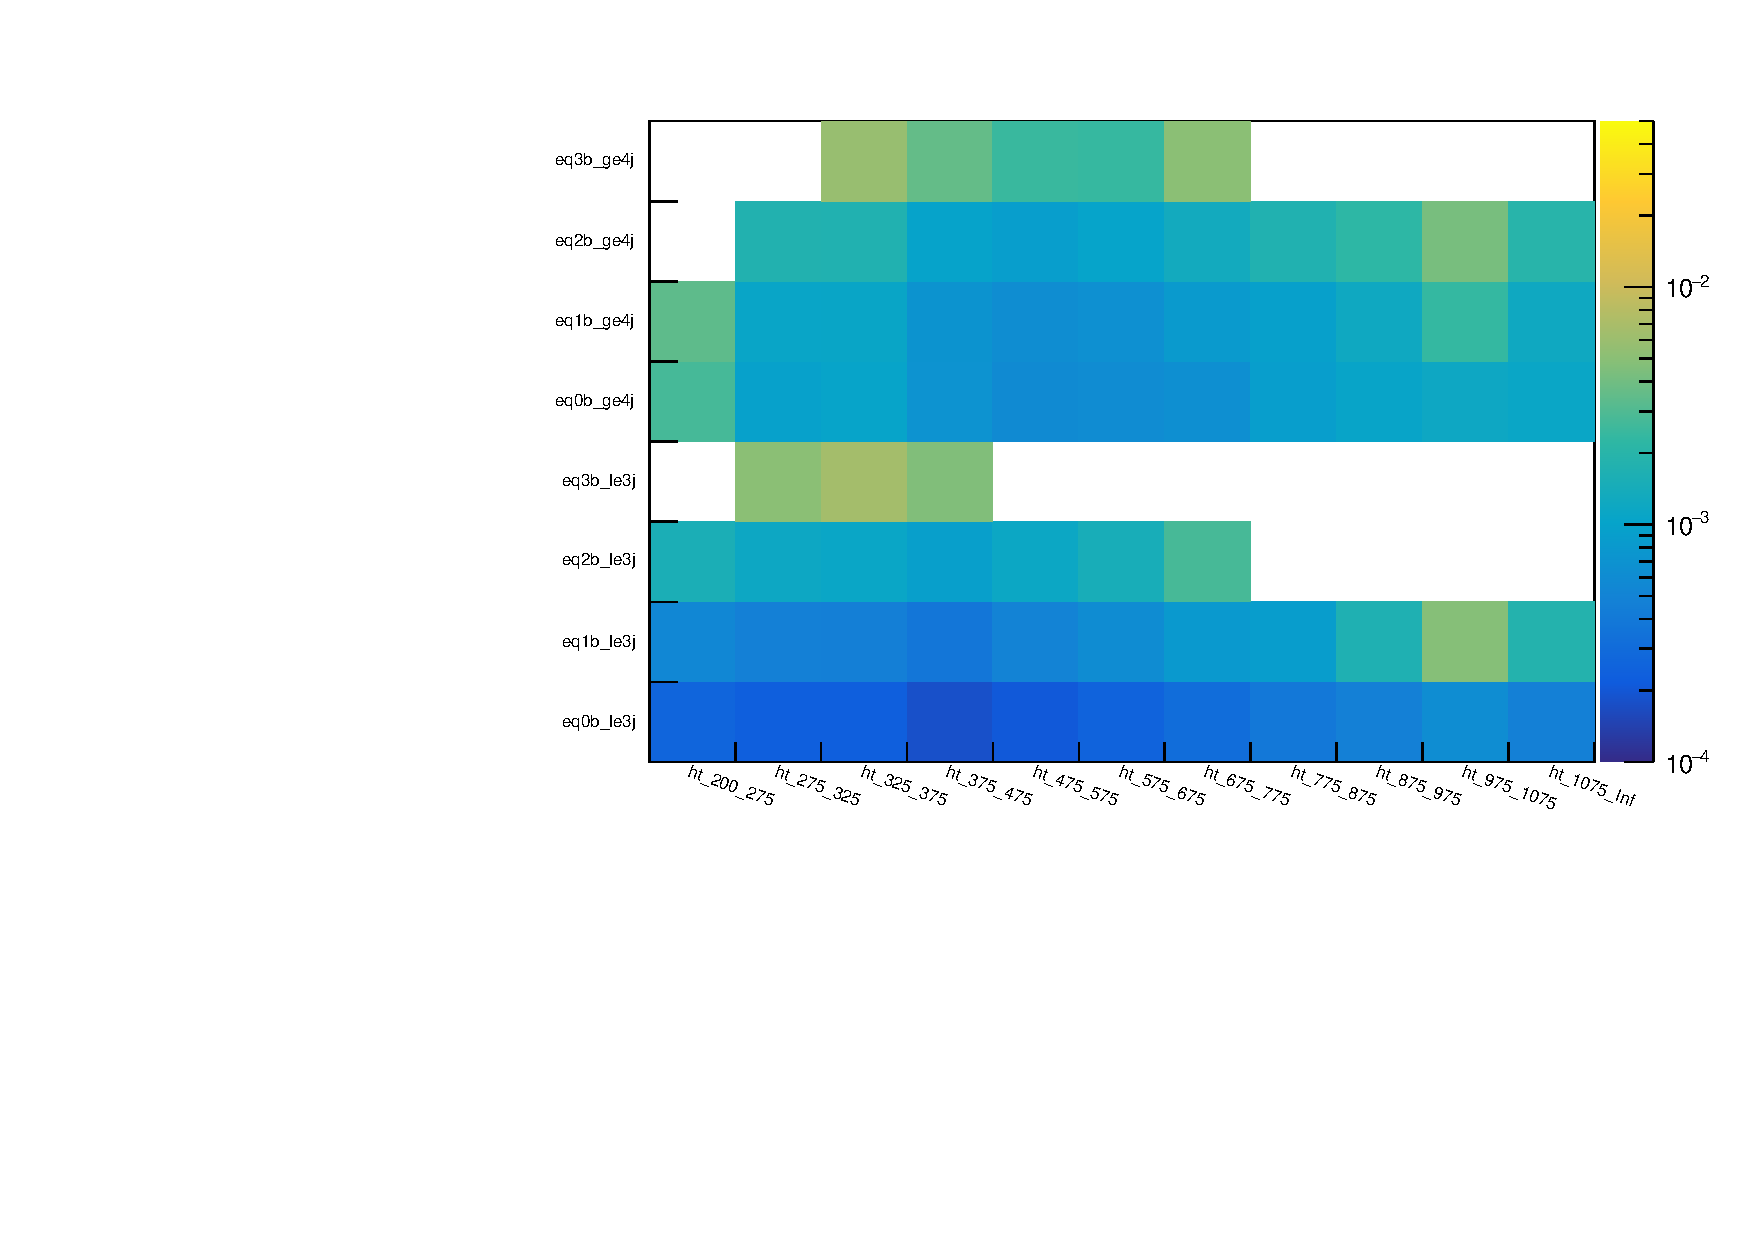
\includegraphics[width=0.5\textwidth]{figures/template/linear/frenchFlagErrCompleteExpected_Linear2D_p1_Ttw.pdf}
  }~~
  \subfigure[\label{fig:observedTtw} Observed uncertainties]{
    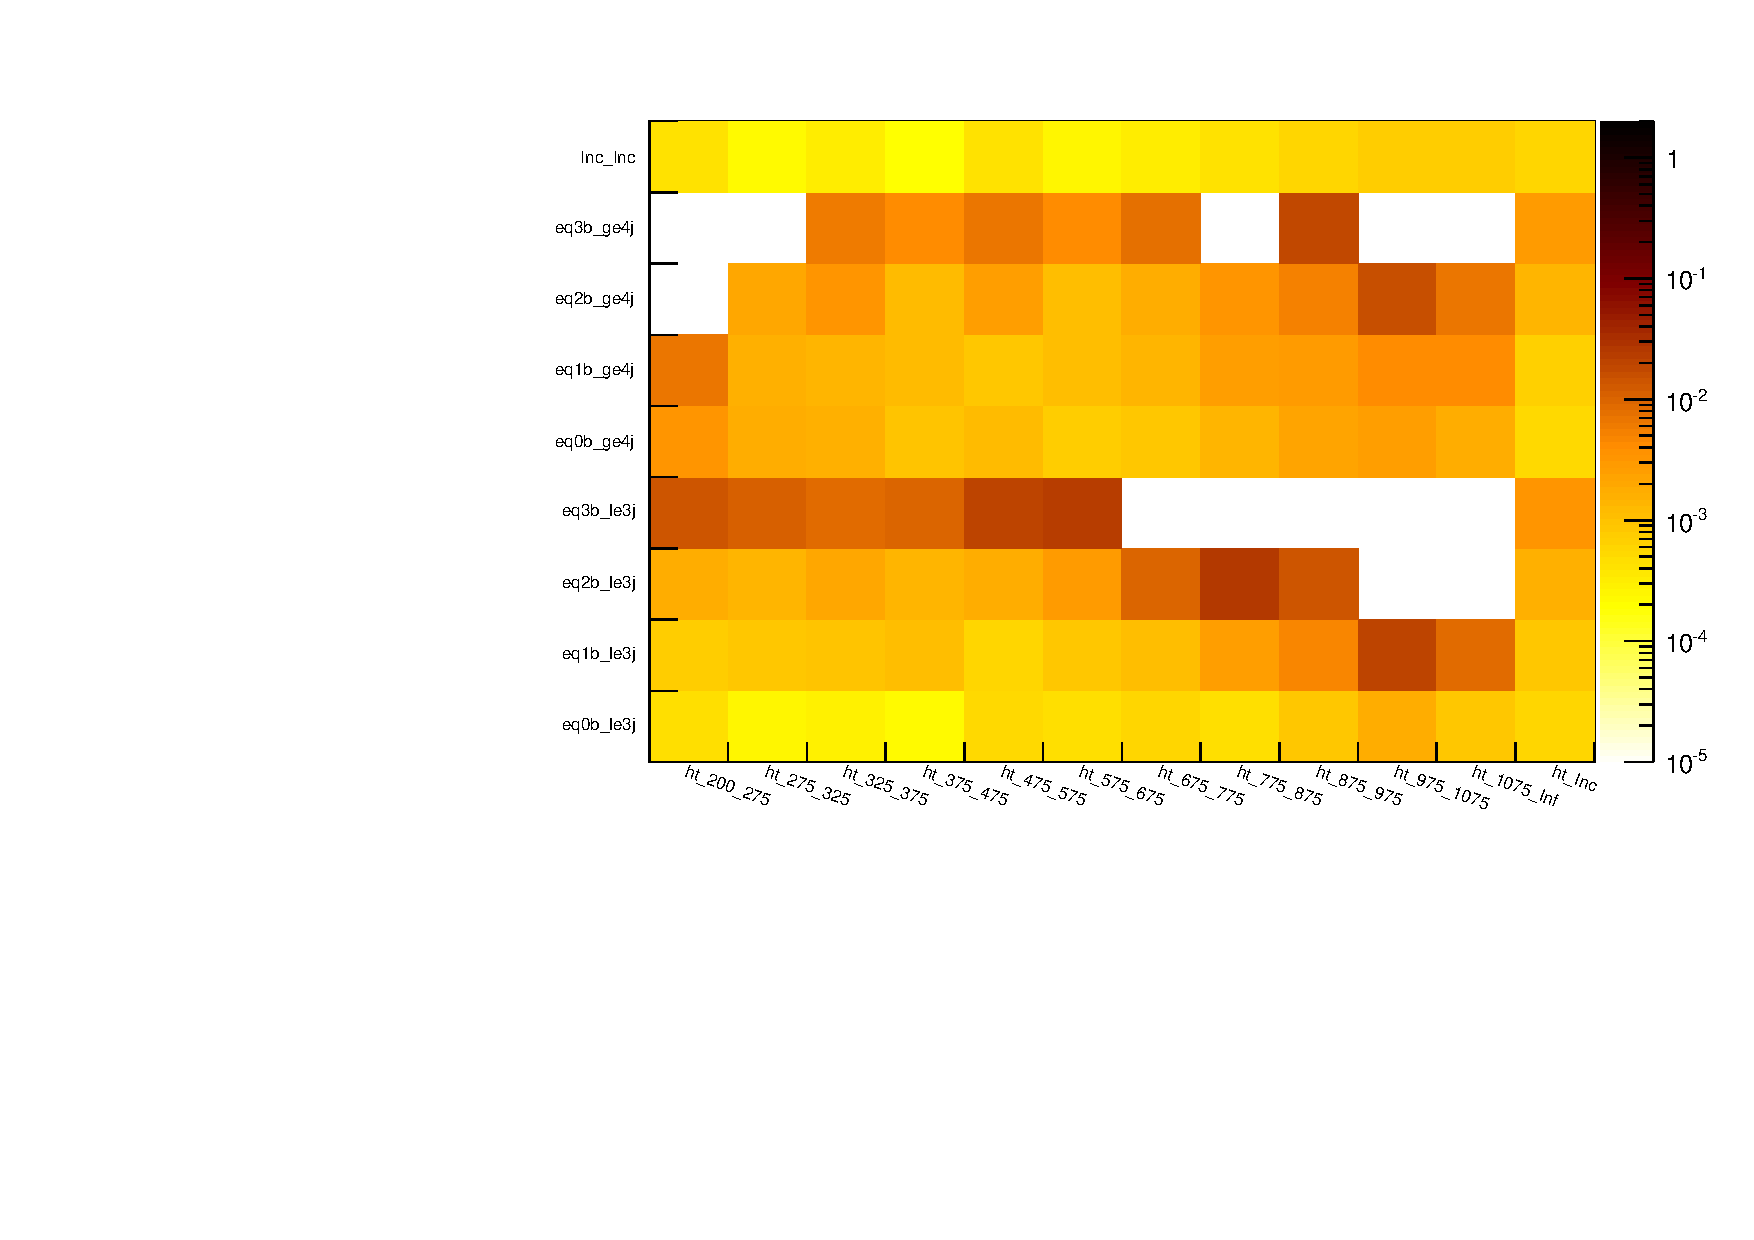
\includegraphics[width=0.5\textwidth]{figures/template/linear/frenchFlagErrComplete_Linear2D_p1_Ttw.pdf}
  }\\
  \caption{\label{fig:expectedObservedTtw} Expected relative uncertainties shown for \ttbar/W in Figure~\ref{fig:expectedTtw} are consistent
  with observed relative uncertainties shown in Figure~\ref{fig:observedTtw}.}
\end{figure}

\begin{figure}[h!]
  \centering
  \subfigure[\label{fig:expectedZinv} Expected uncertainties]{
    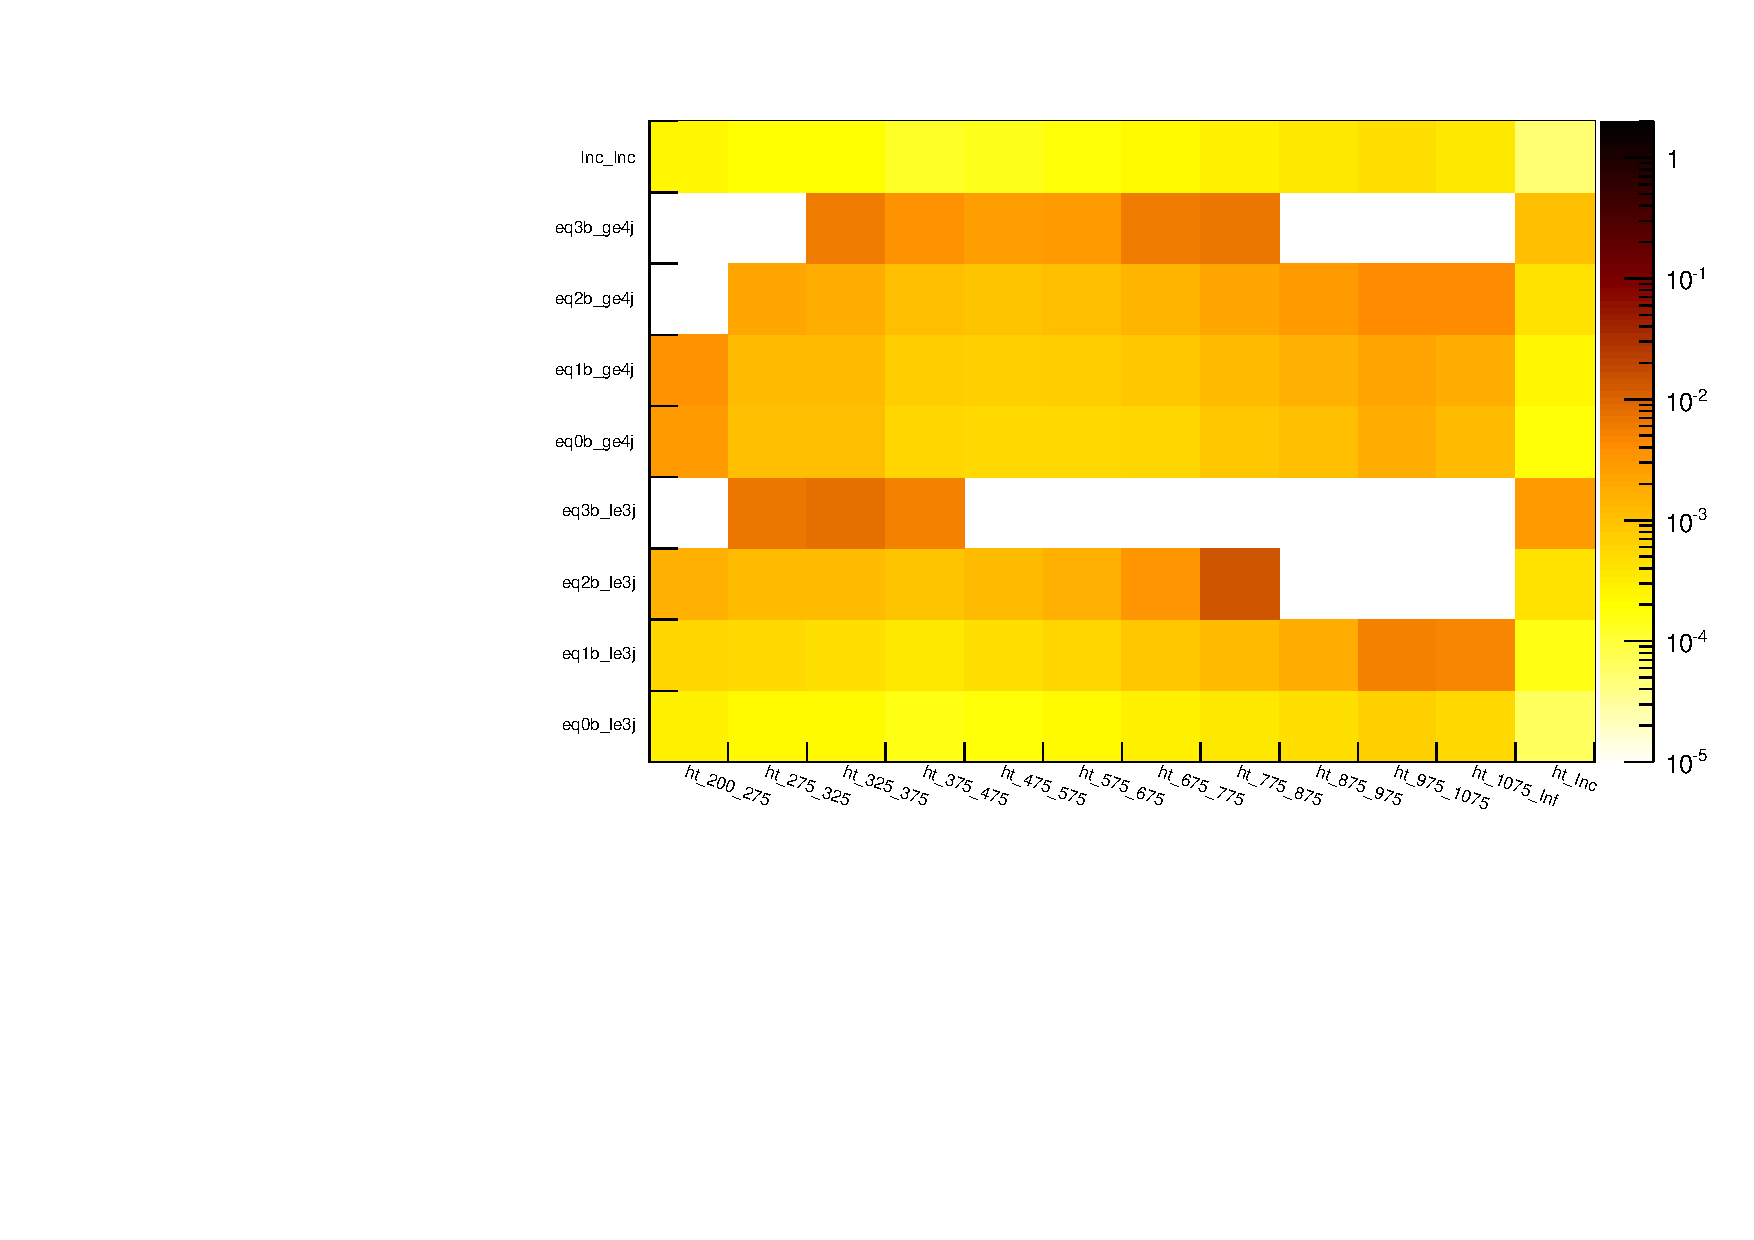
\includegraphics[width=0.5\textwidth]{figures/template/linear/frenchFlagErrCompleteExpected_Linear2D_p1_Zinv.pdf}
  }~~
  \subfigure[\label{fig:observedZinv} Observed uncertainties]{
    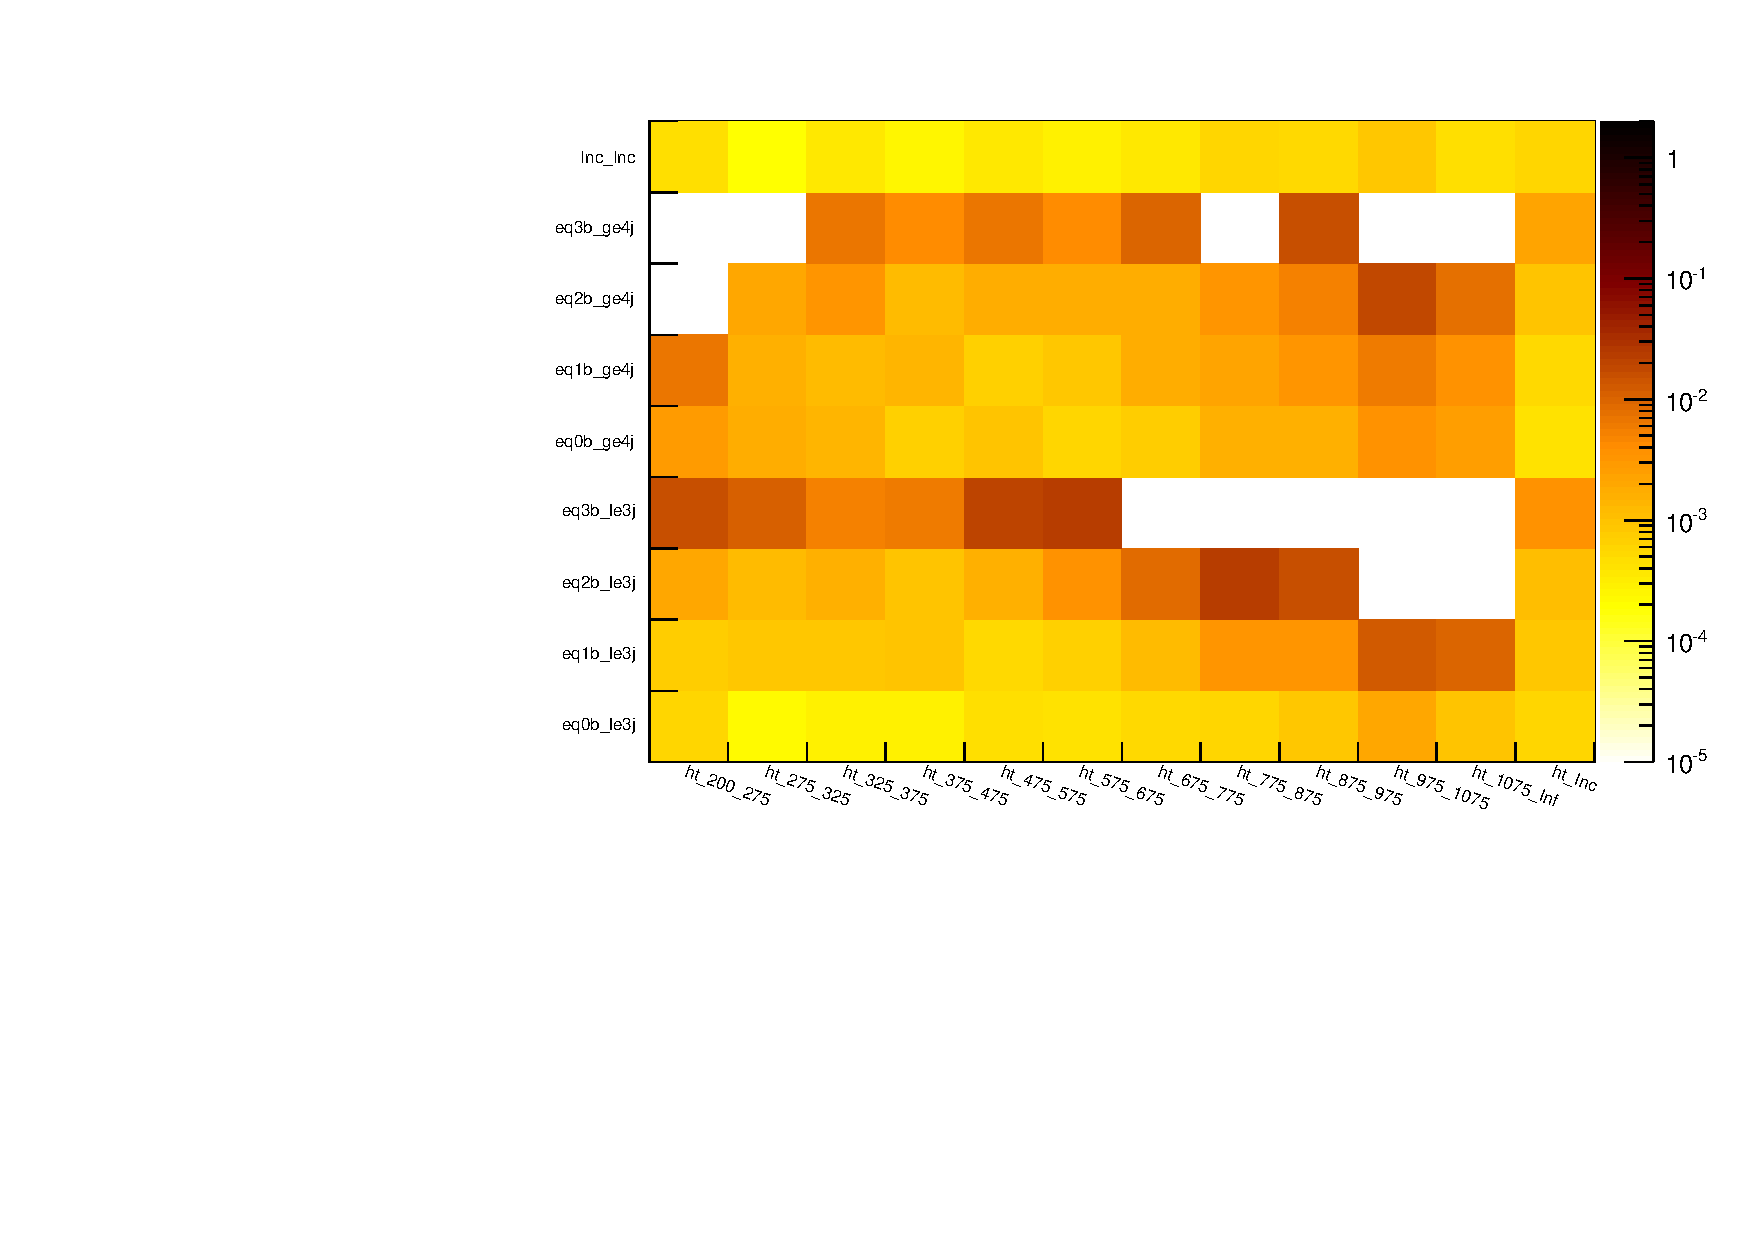
\includegraphics[width=0.5\textwidth]{figures/template/linear/frenchFlagErrComplete_Linear2D_p1_Zinv.pdf}
  }\\
  \caption{\label{fig:expectedObservedZinv}Expected relative uncertainties shown for \zInv~ in Figure~\ref{fig:expectedZinv} are consistent
  with observed relative uncertainties shown in Figure~\ref{fig:observedZinv}.}
\end{figure}

\subsection{Validation with 13\texorpdfstring{\TeV} data}
\label{sec:dataValid13TeV}
The scale anchoring approach has been validated with 552\ipb 
of data collected at 13\TeV. In Figure~\ref{fig:pulls13} the 
pulls of the linear parameter for the combined fit over
the control regions used for the \ttbar/W prediction (\mj)
and for \zInv~ (\mj, \mmj, \gj) are shown to be consistent with no bias.
In Figure~\ref{fig:frenchFlagPulls13} the french flag plot of the pulls
also shows no regions with consistent bias for either background.
Finally, figure Figure~\ref{fig:expectedObservedTtw} and Figure~\ref{fig:expectedObservedTtw}
show the observed systematics agree well with those expected as 
was observed in the full 8\TeV dataset. These validations will
be continually updated as additional data becomes available.

\begin{figure}[h!]
  \centering
  \subfigure[\gj]{
    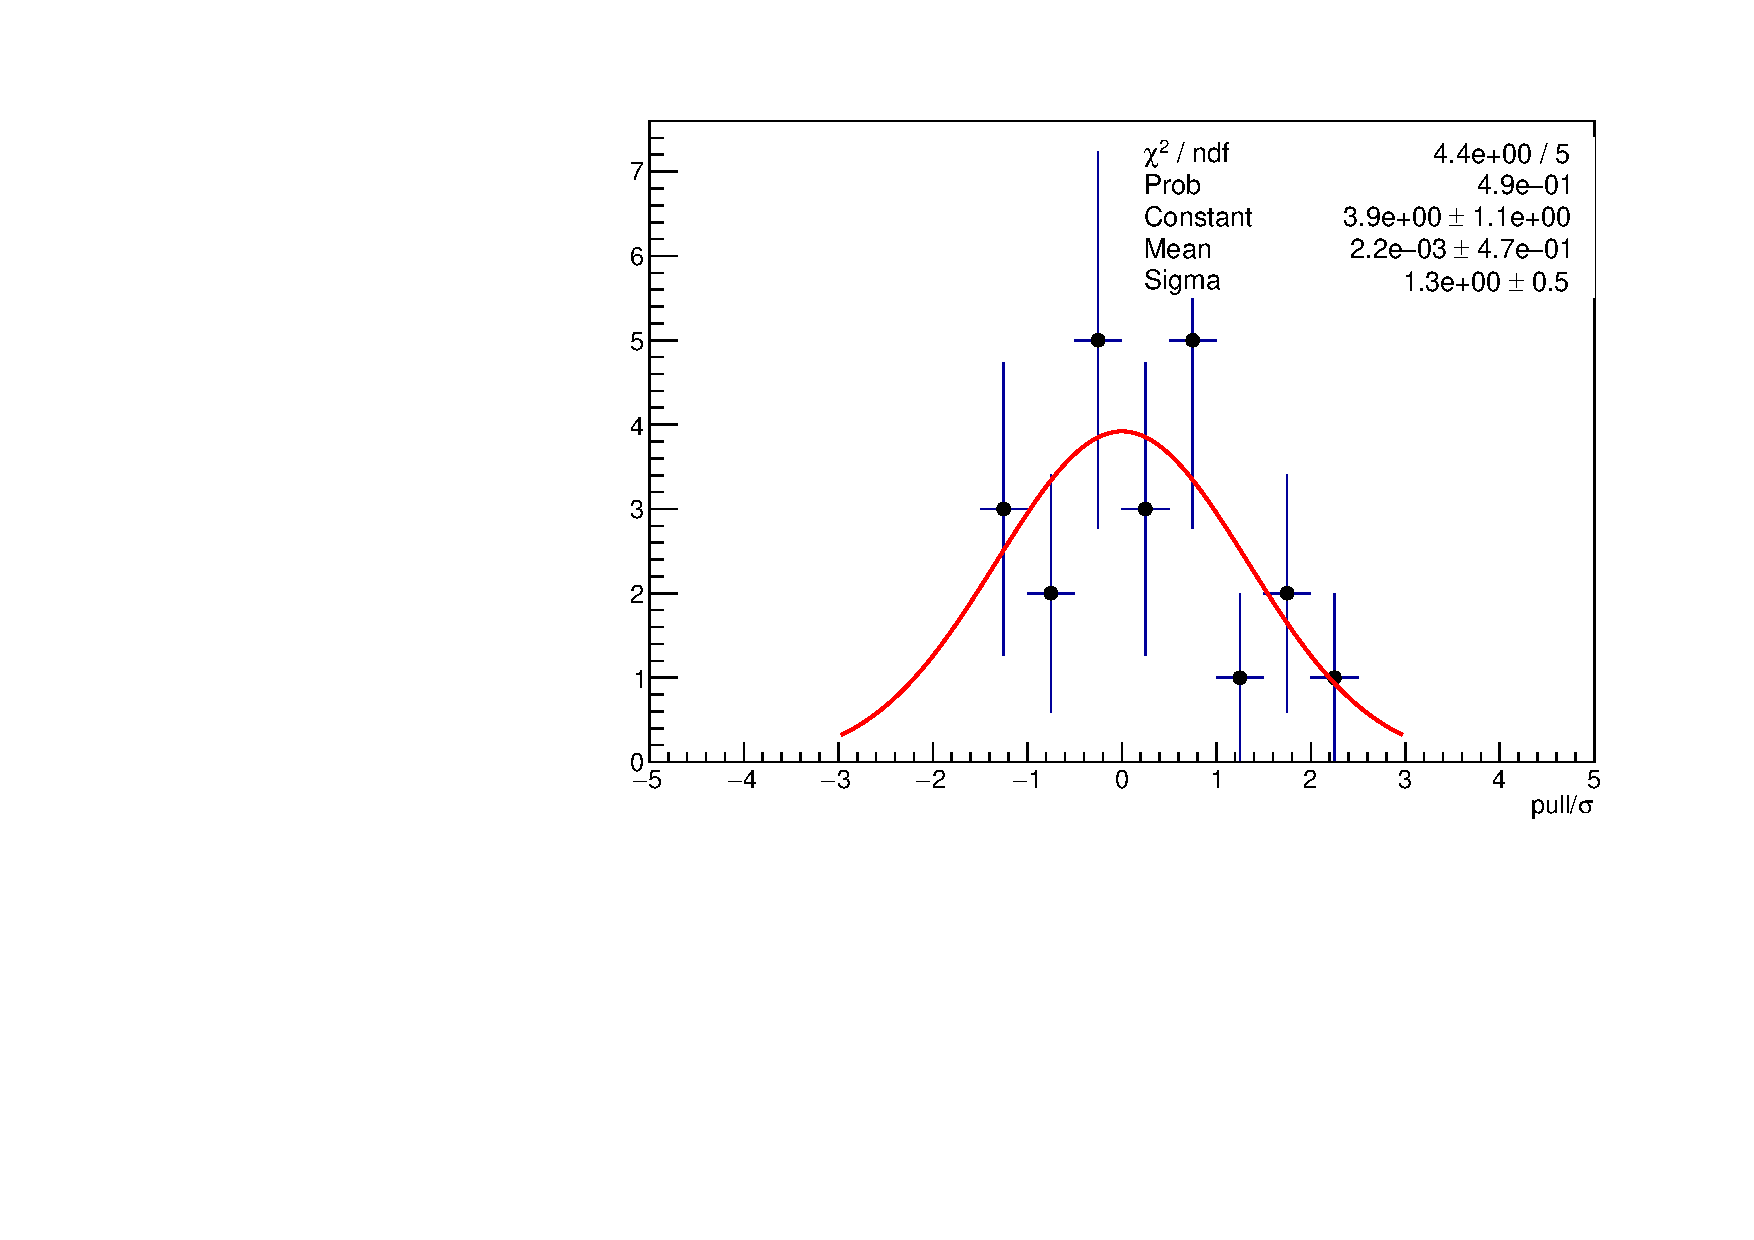
\includegraphics[width=0.5\textwidth]{figures/template13TeV/550pb/pull_Linear2DShiftMean_p1_SinglePhoton.pdf}
  }~~
  \subfigure[\mmj]{
    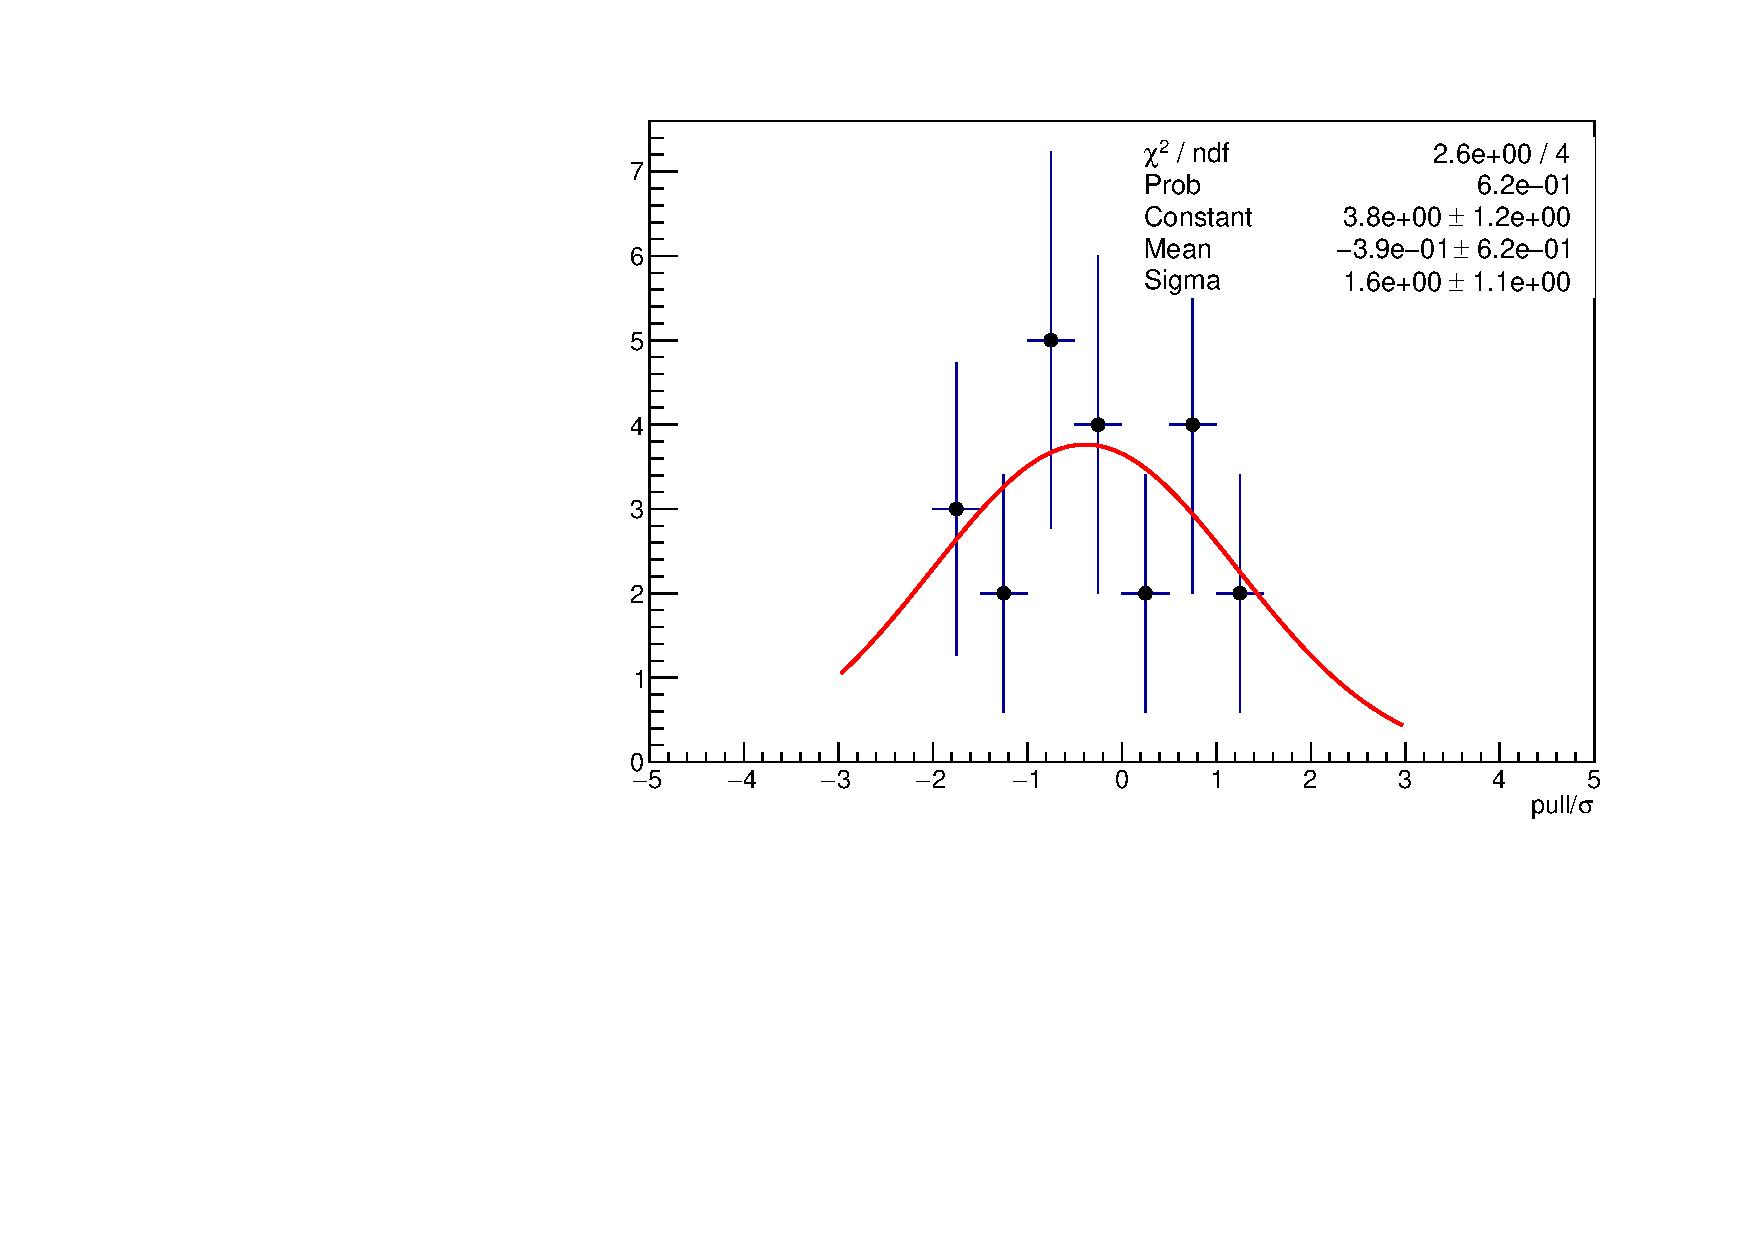
\includegraphics[width=0.5\textwidth]{figures/template13TeV/550pb/pull_Linear2DShiftMean_p1_DoubleMu.pdf}
  }\\
  \subfigure[\mj]{
    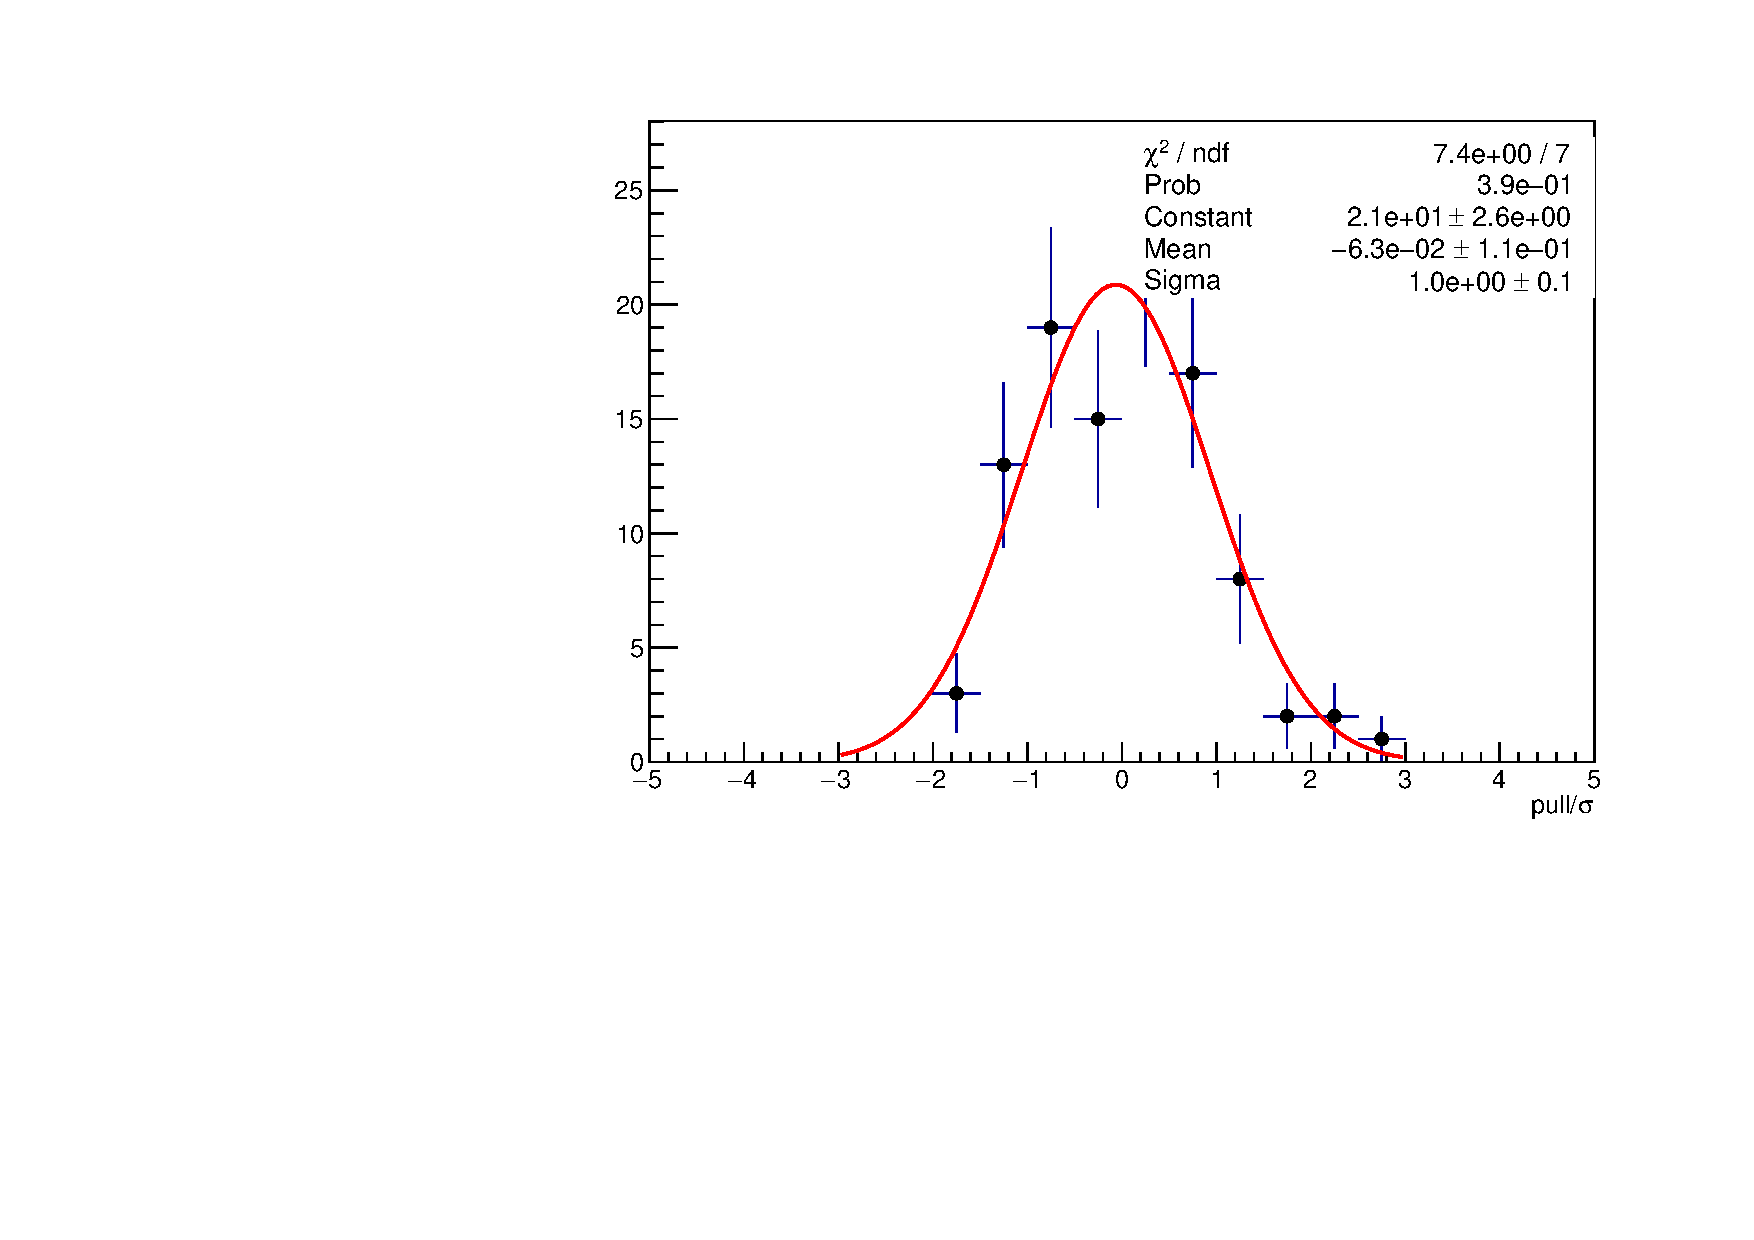
\includegraphics[width=0.5\textwidth]{figures/template13TeV/550pb/pull_Linear2DShiftMean_p1_SingleMu.pdf}
  }~~
  \\
  \caption{\label{fig:pulls} 
  The pull distribution of the linear parameter from the flat hypothesis showing no significant bias for any control region.}
\end{figure}
\begin{figure}[h!]
  \centering
  \subfigure[\gj]{
    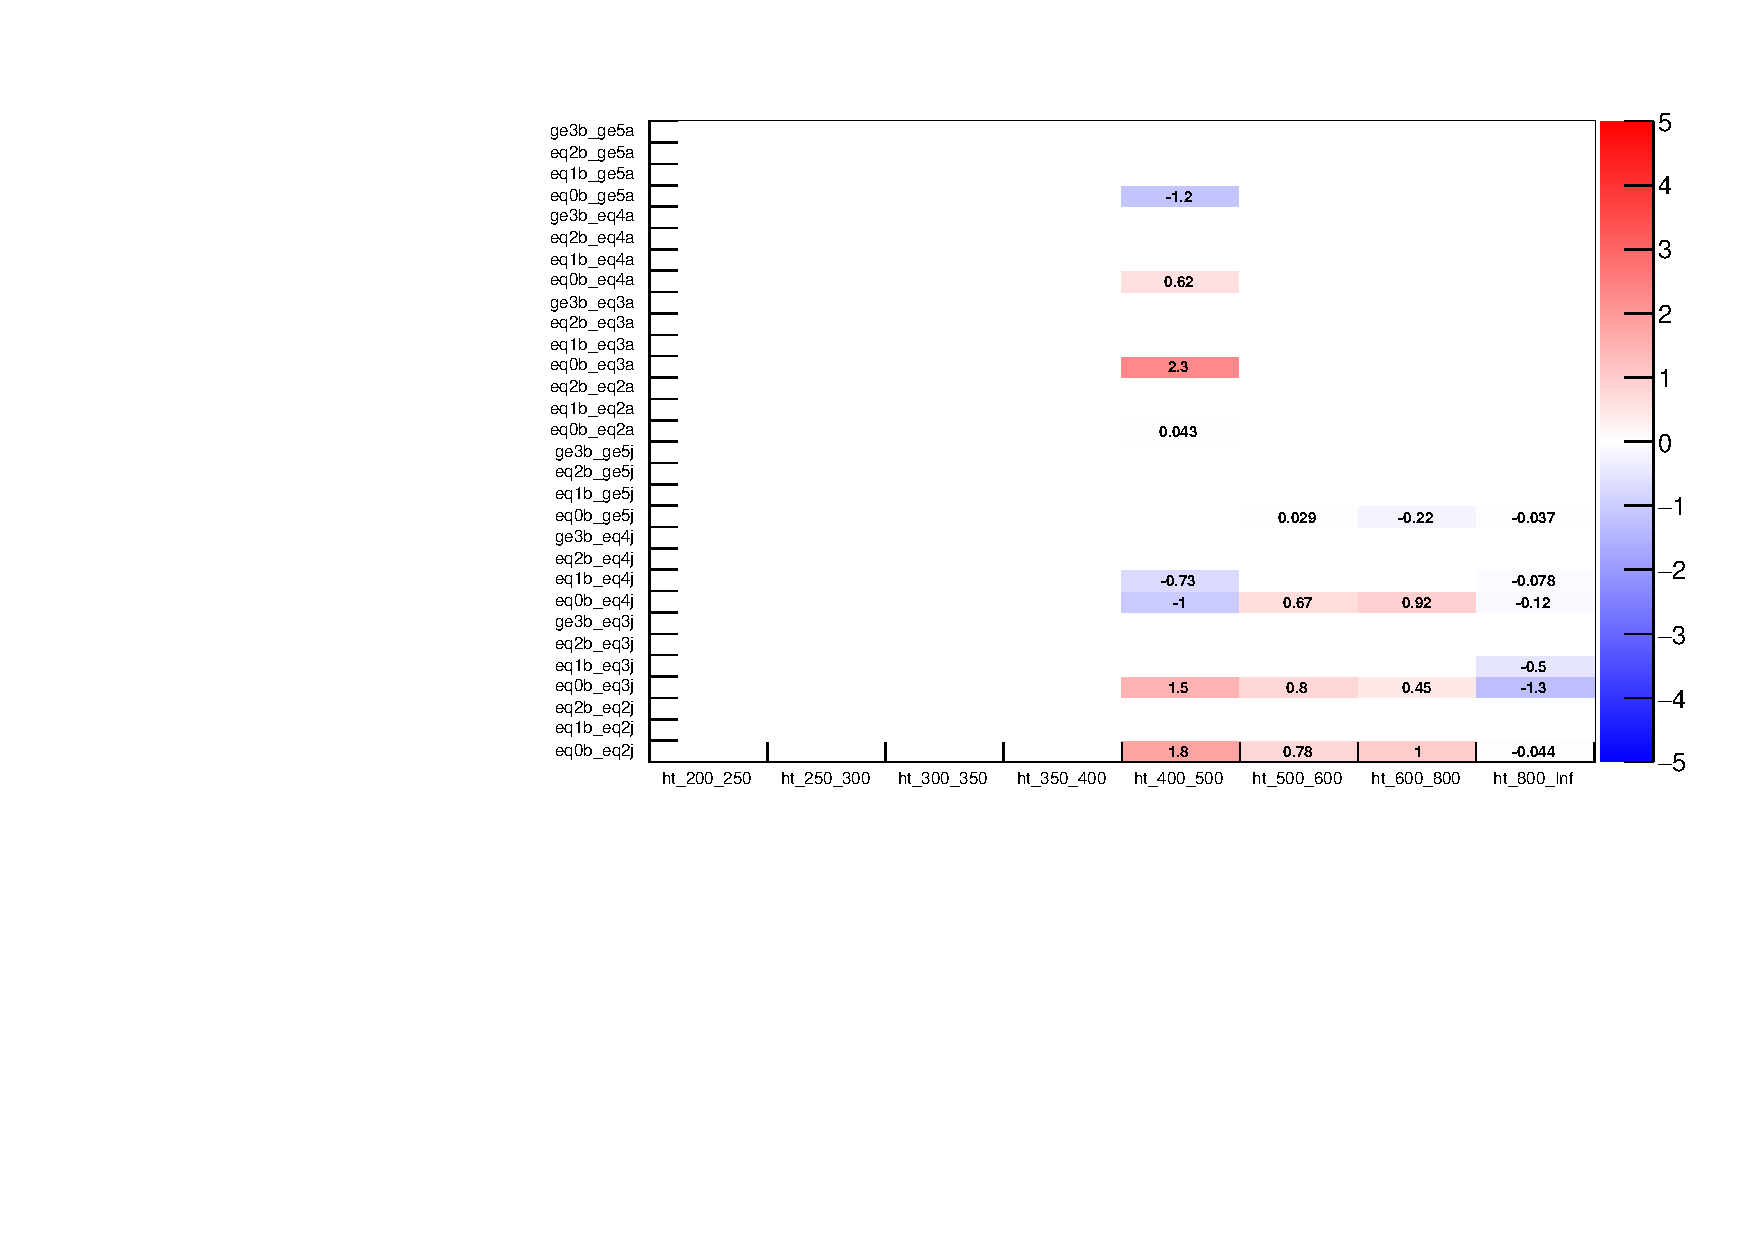
\includegraphics[width=0.5\textwidth]{figures/template13TeV/550pb/frenchFlagPull_Linear2DShiftMean_p1_SinglePhoton.pdf}
  }~~
  \subfigure[\mmj]{
    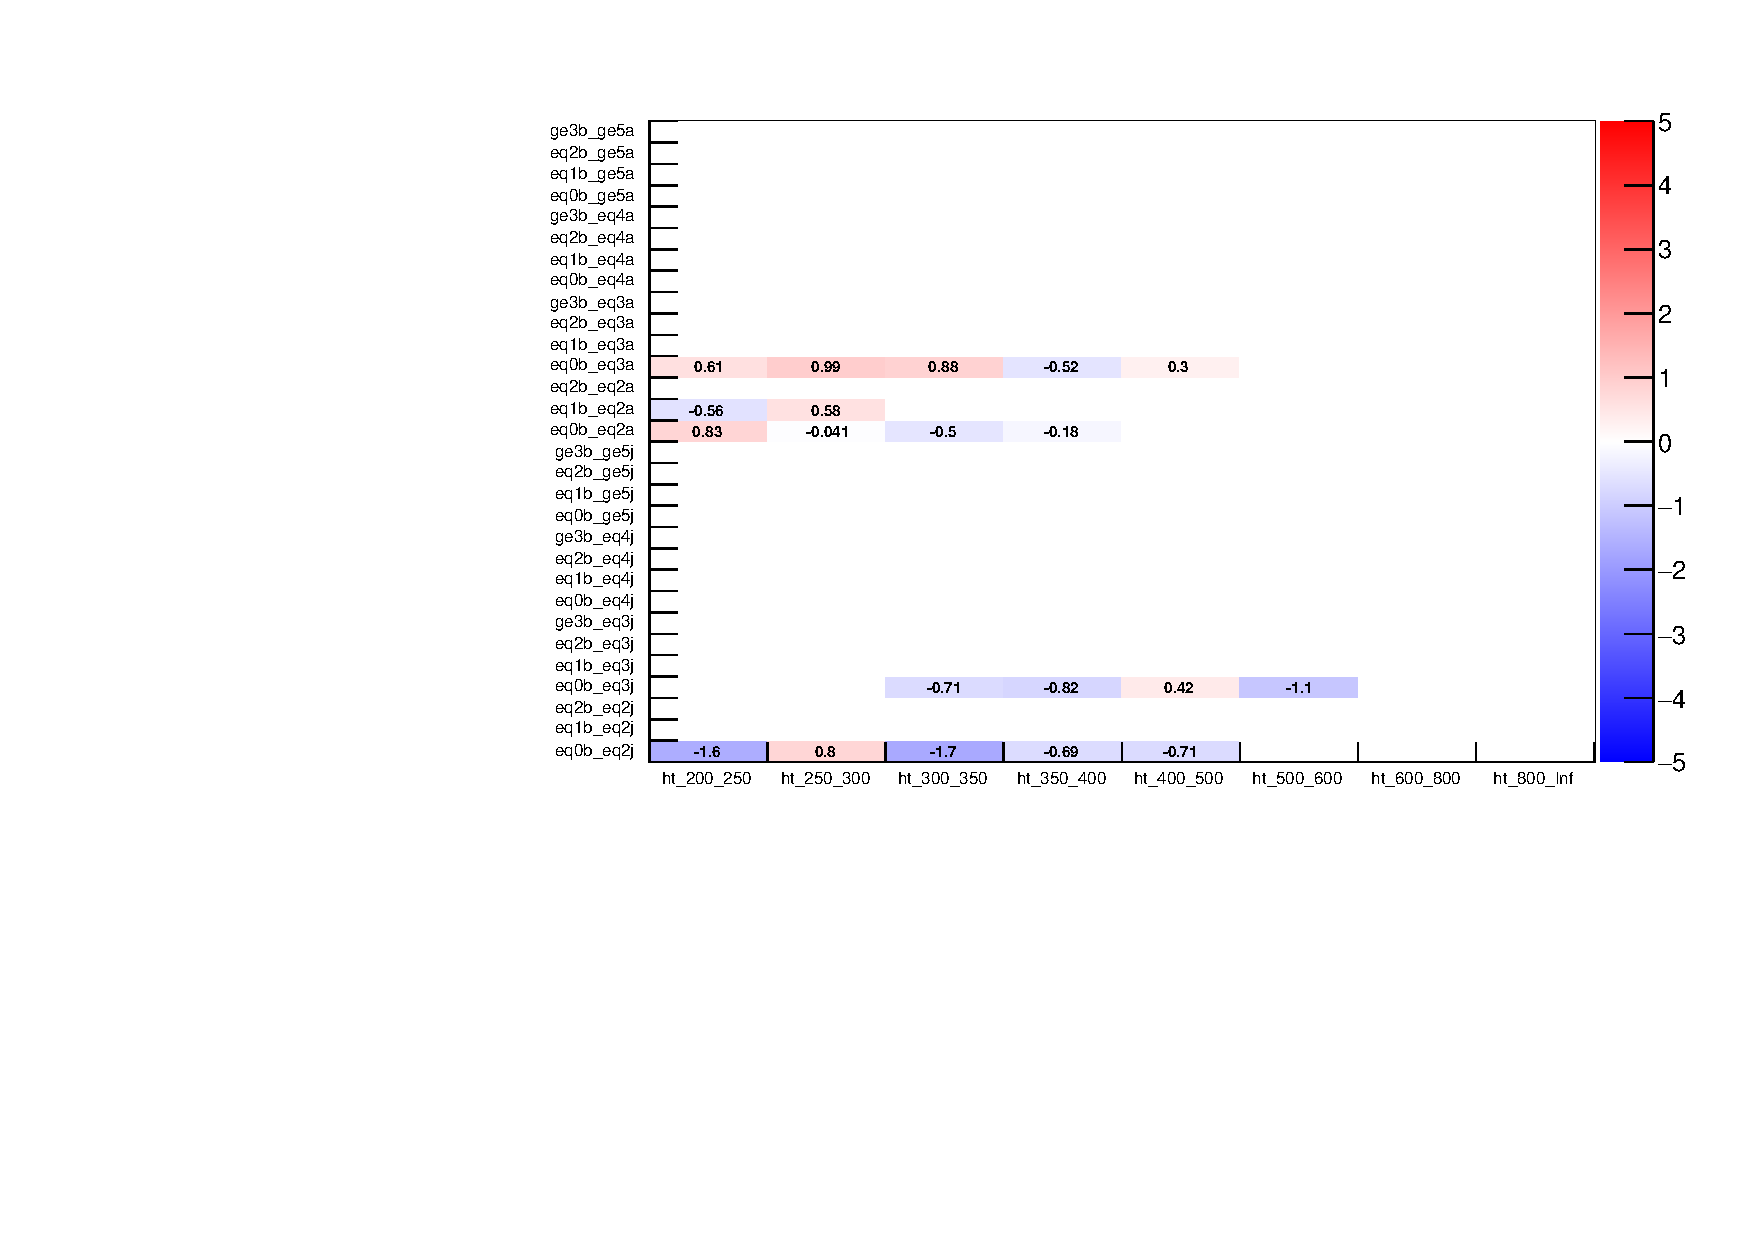
\includegraphics[width=0.5\textwidth]{figures/template13TeV/550pb/frenchFlagPull_Linear2DShiftMean_p1_DoubleMu.pdf}
  }\\
  \subfigure[\mj]{
    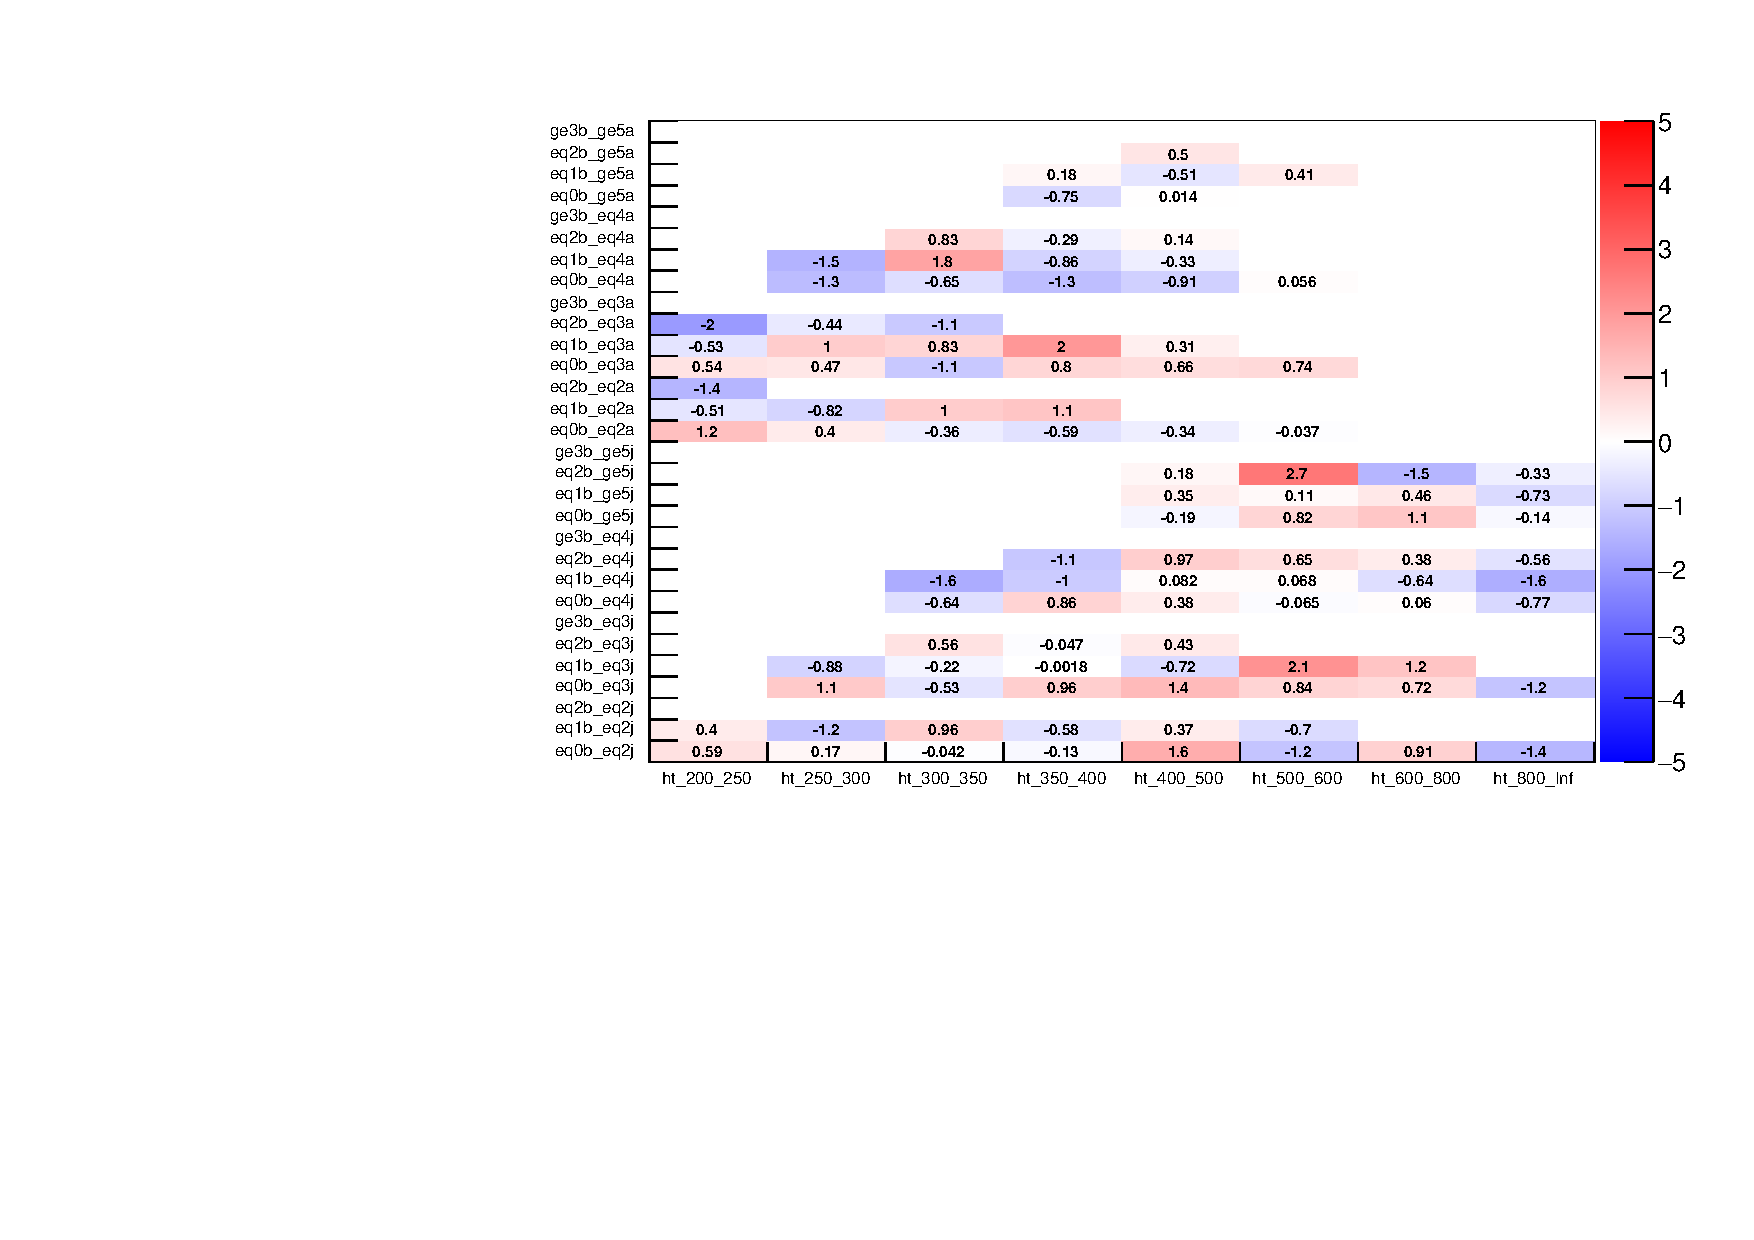
\includegraphics[width=0.5\textwidth]{figures/template13TeV/550pb/frenchFlagPull_Linear2DShiftMean_p1_SingleMu.pdf}
  }~~
  \\
  \caption{\label{fig:frenchFlagPulls} The pull distribution of the linear parameter from the flat hypothesis across all
  \scalht bins and categories. There are no significant pulls for the \scalht binned
  fits while the \scalht inclusive case shows very large pulls as expected. 
  Due to trigger requirements the \gj control sample may only be used for \scalht $> 400$\GeV.}
\end{figure}
\subsection{Bias injection test}

\label{sec:biasInj}
To understand the effect of a bias which effects only very high 
\mht bins on the validation procedure a bias injection test is carried out.
The prediction in the final bin only is varied and the effect on the 
overall pull studied. The results are shown for the symmetric jet categories only
as for asymmetric categories the final \mht bin dominates the fit. This is 
an extreme test of the ability to probe bias using the linear fit. 
Figure~\ref{fig:biasInjTest} displays the results of this test showing
the pull distribution is sensitive to such a bias. In Figure~\ref{fig:biasSyst} the 
change in predicted systematic is shown for the case of halving the prediction in the last bin. 
This shows an overall substantial increase in the systematics predicted.

\begin{figure}[]
  \centering
  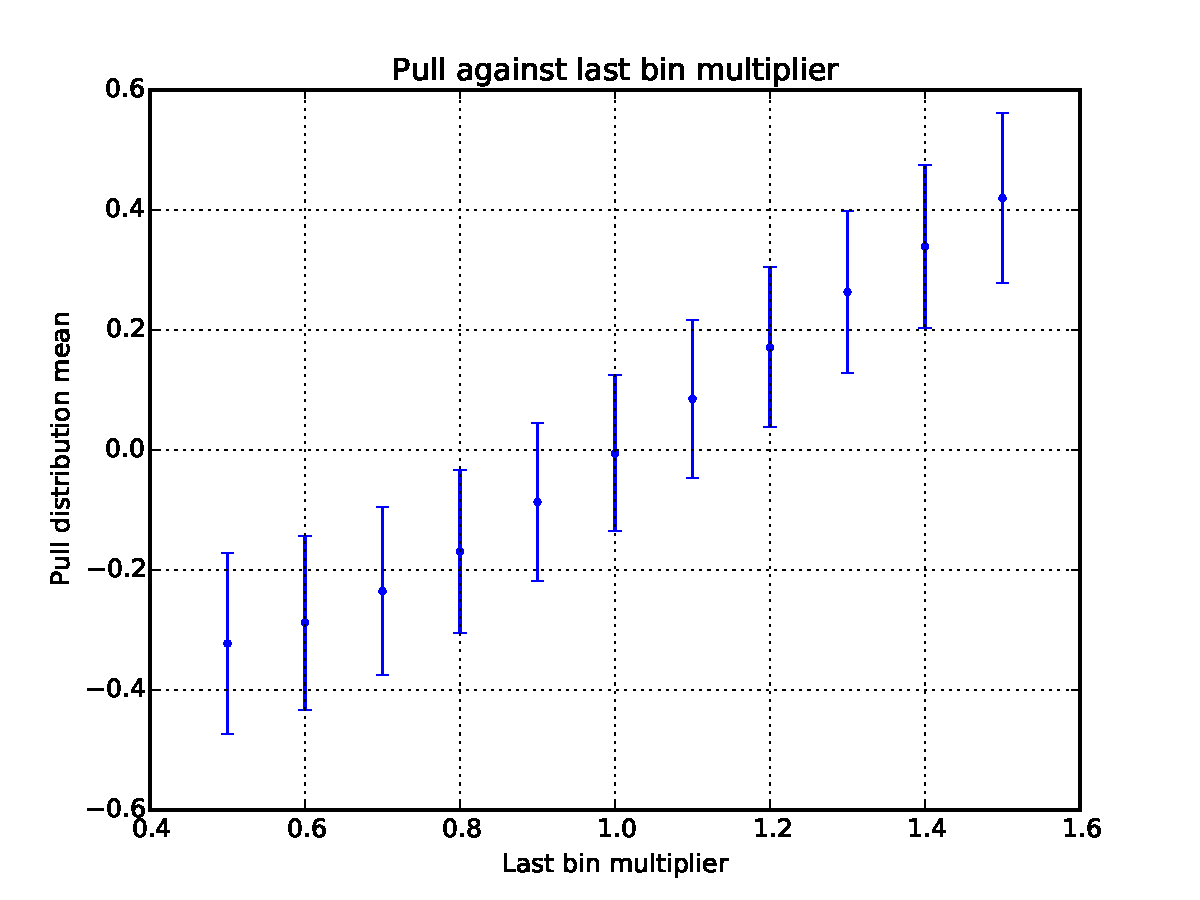
\includegraphics[width=0.5\textwidth]{figures/template/biasInjTest.pdf}
  \caption{\label{fig:biasInjTest} Mean pull against last bin multiplier for 
  the \mj control region showing the linear polynomial is sensitive to a bias effecting the final bin only.}
\end{figure}

\begin{figure}[]
  \centering
  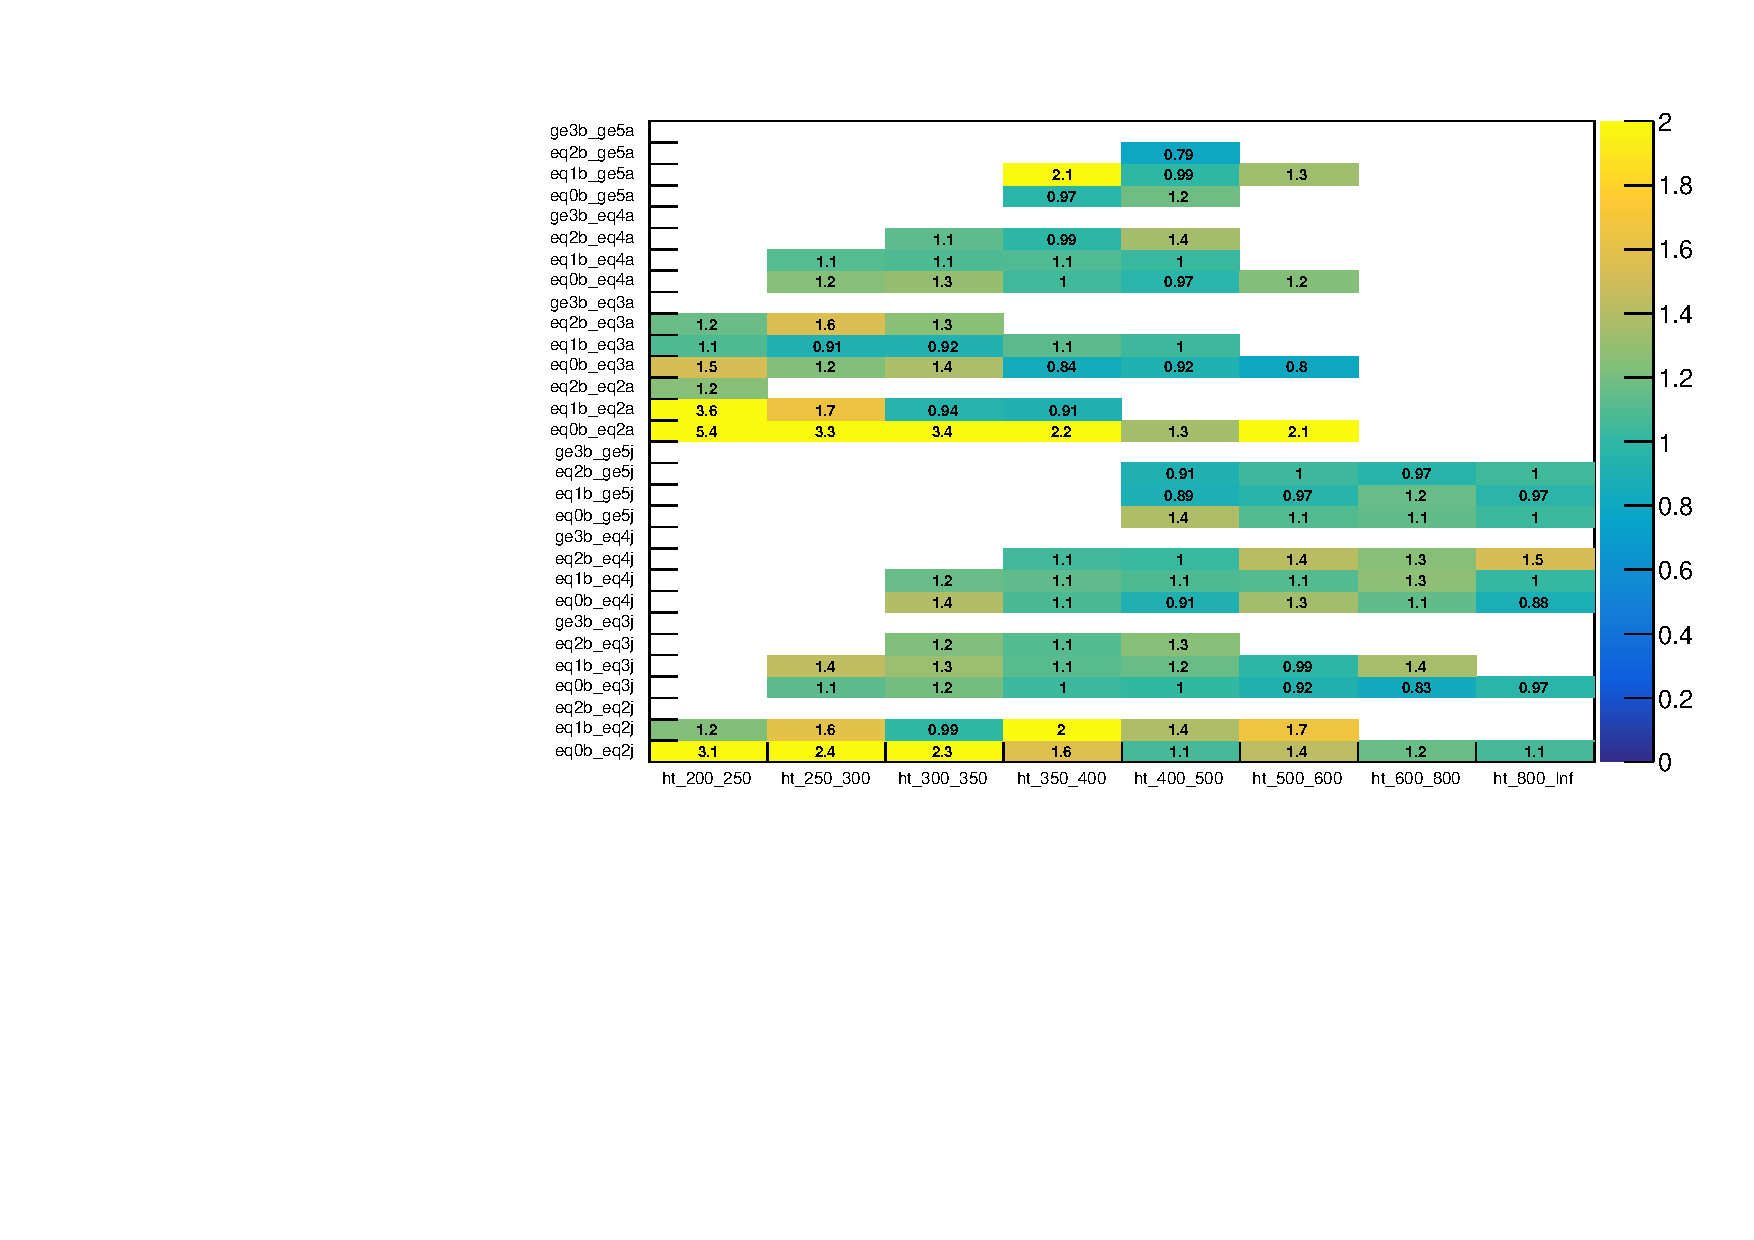
\includegraphics[width=0.5\textwidth]{figures/template/biasSystTest.pdf}
  \caption{\label{fig:biasSyst} Change in systematic parameter when the prediction in the last bin
  is halved}
\end{figure}

\subsection{Expected systematic uncertainties for the 13 \texorpdfstring{\TeV} analysis}
\label{sec:syst13TeV}
Using the method described in Section~\ref{sec:systMhtDimension} the expected uncertainties
from 13 \TeV MC for both \ttbar/W  and \zInv~ using all relevant control regions are
shown in Figure~\ref{fig:expected13} for 3\ifb. 
Depending on the category and \scalht bin, uncertainties between 1 and 10\% are found
on the linear parameter.
An example of the overall uncertainties on the \mht templates is shown
in Figure~\ref{fig:exampleTemplate13}.
The alternative templates derived with this method are folded into the 
likelihood described in Section~\ref{sec:likelihood} to account for
systematic uncertainties in the \mht dimension.
As a gauge of the effect of the template variations the uncertainty parameter 
can be translate to an uncertainty on the last bin. This is typically
of the order of 10\% depending on the category and is shown
in Figure~\ref{fig:frenchFlagLastBin}.


\begin{figure}[h!]
  \centering
  \subfigure[\label{fig:ttw13} \ttbar/W]{
    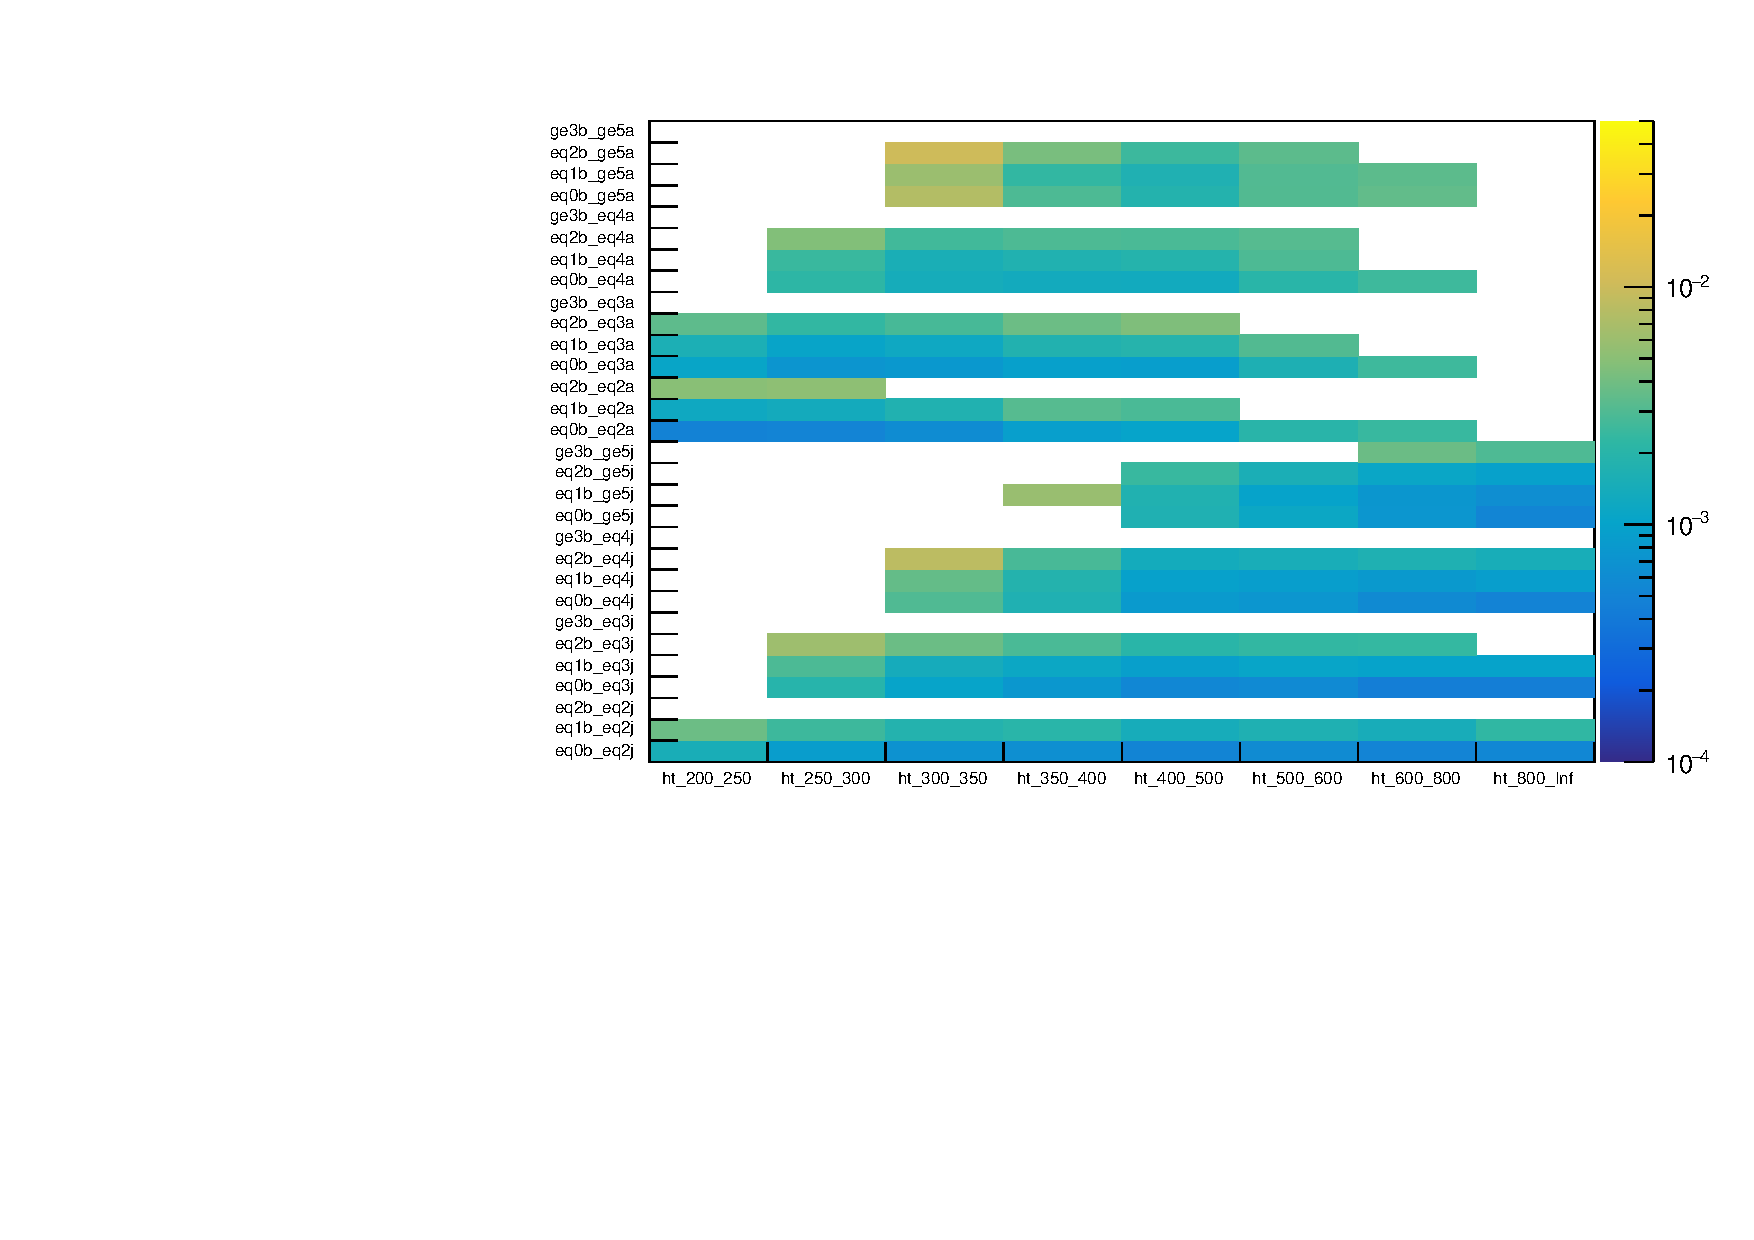
\includegraphics[width=0.5\textwidth]{figures/template13TeV//3fb/frenchFlagErrComplete_Linear2DShiftMean_p1_Ttw.pdf}
  }~~
  \subfigure[\label{fig:zinv13} \zInv~]{
    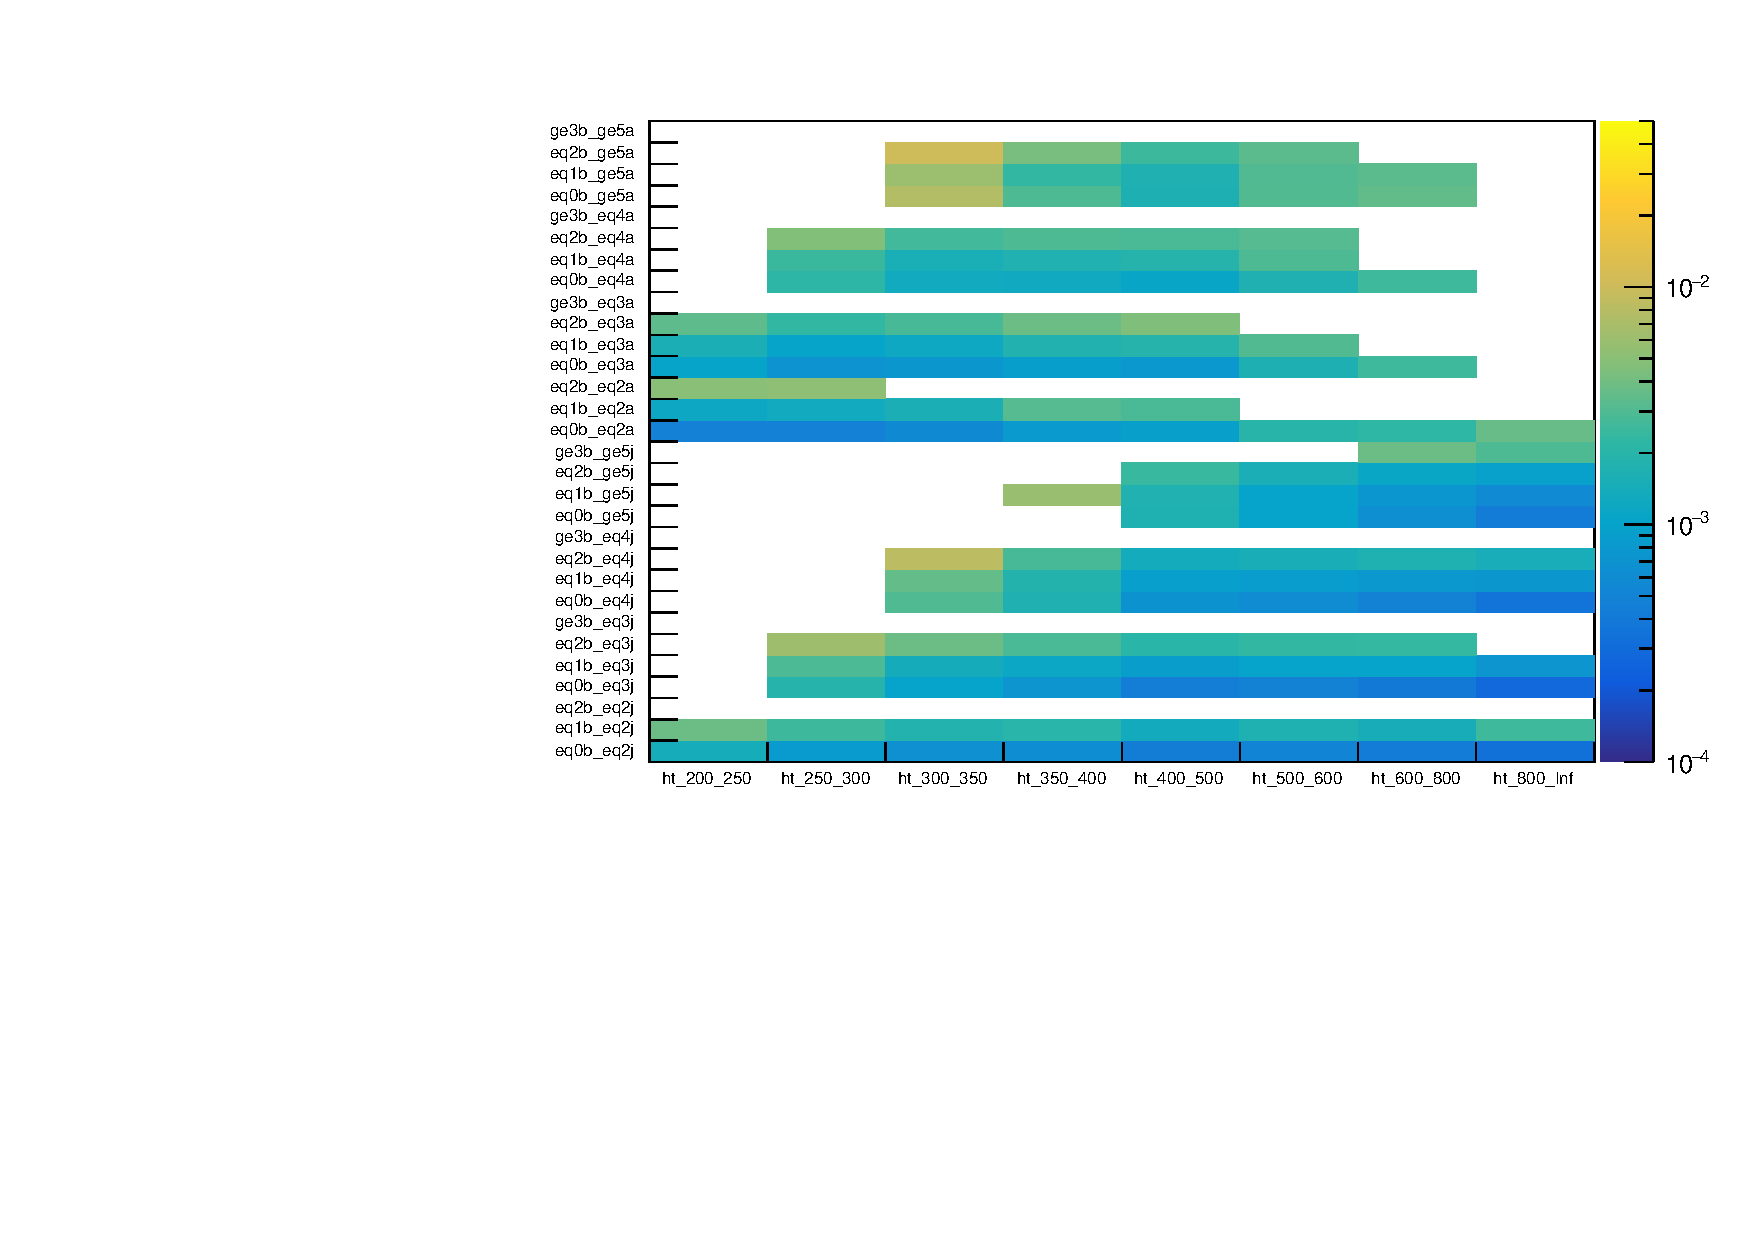
\includegraphics[width=0.5\textwidth]{figures/template13TeV/3fb/frenchFlagErrComplete_Linear2DShiftMean_p1_Zinv.pdf}
  }\\
  \caption{\label{fig:expected13} Expected relative uncertainties on the template shown for \zInv~ in Figure~\ref{fig:zinv13} 
  and \ttbar/W in Figure~\ref{fig:ttw13} are around 1 to 10\%.}
  
\end{figure}
\begin{figure}[]
  \centering
  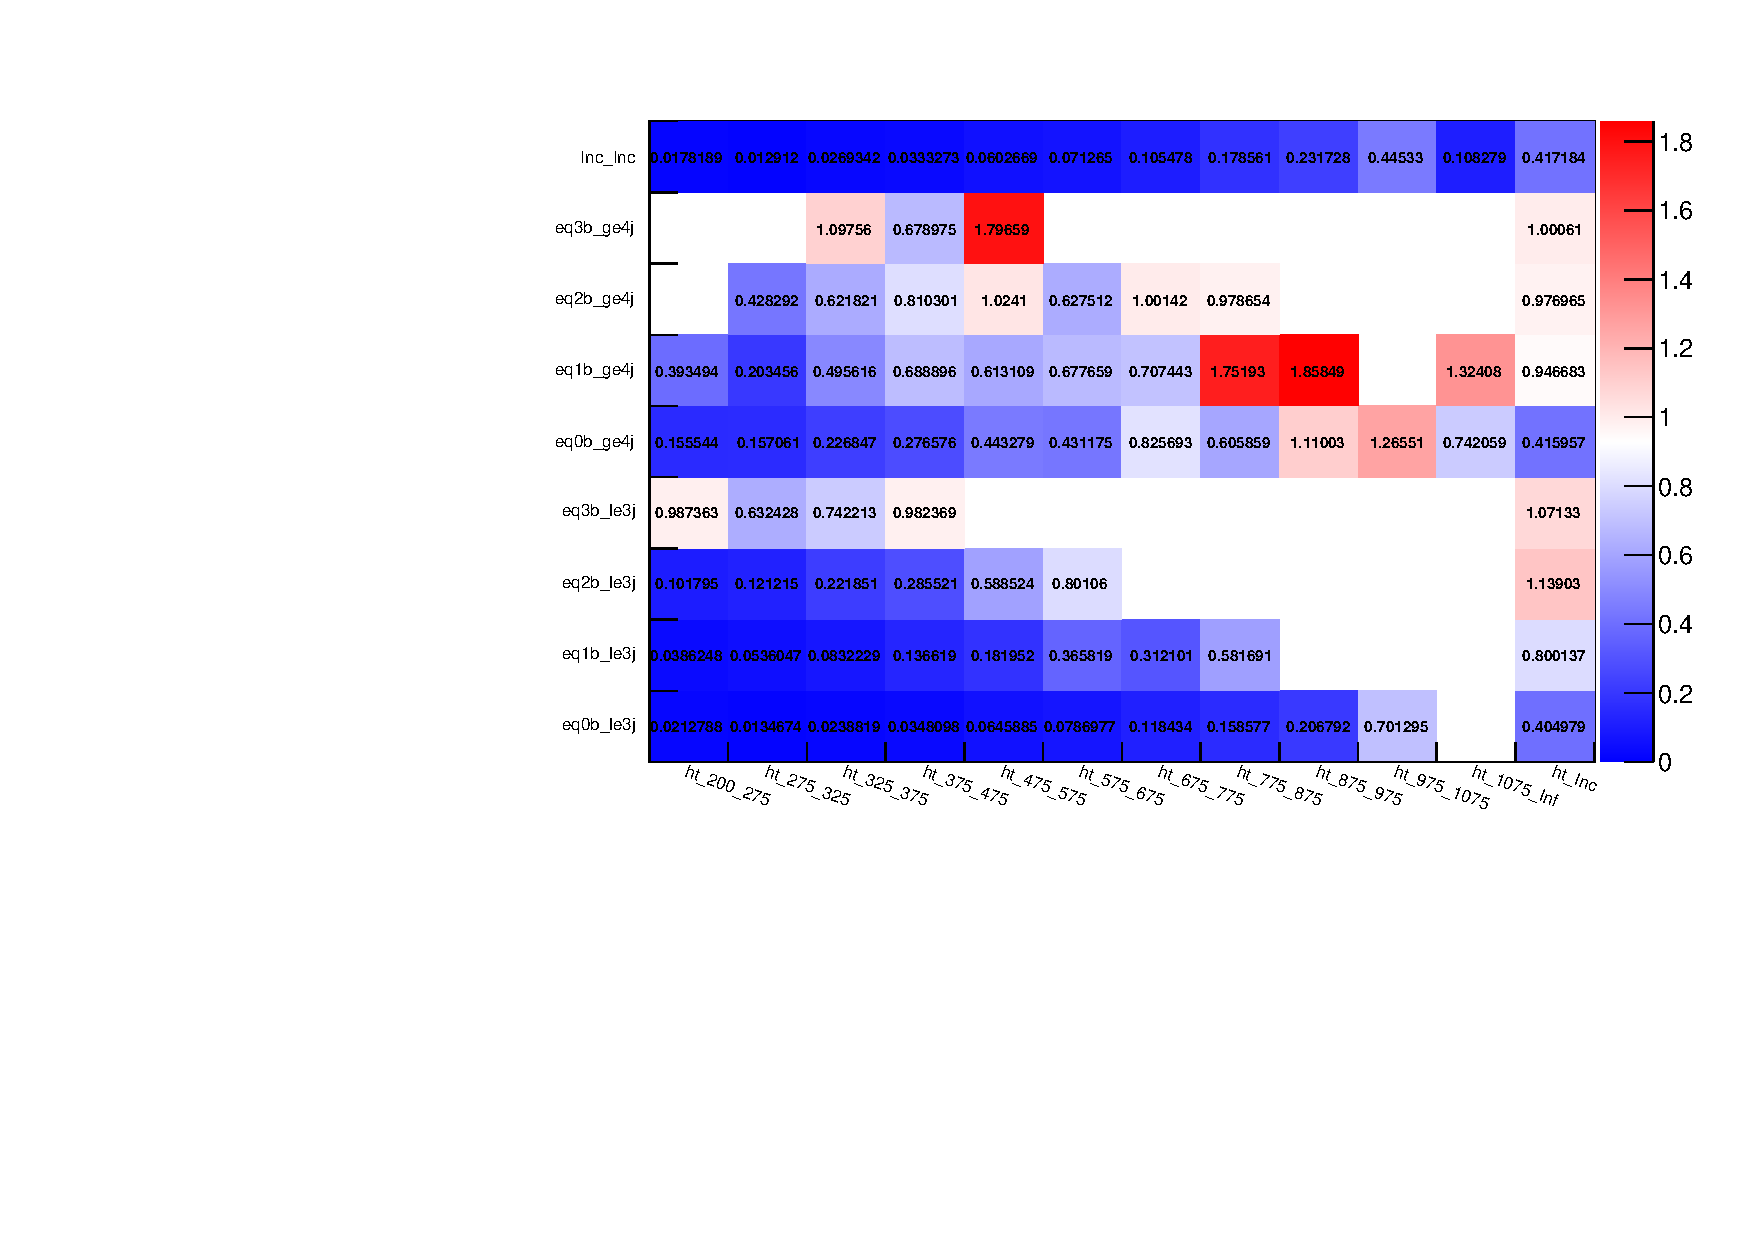
\includegraphics[width=0.5\textwidth]{figures/template/frenchFlagLastBin.pdf}
  \caption{\label{fig:frenchFlagLastBin} Expected uncertanties on the final bin
over all categories and \scalht bins for 3\ifb.}
\end{figure}

\begin{figure}[h!]
  \centering
  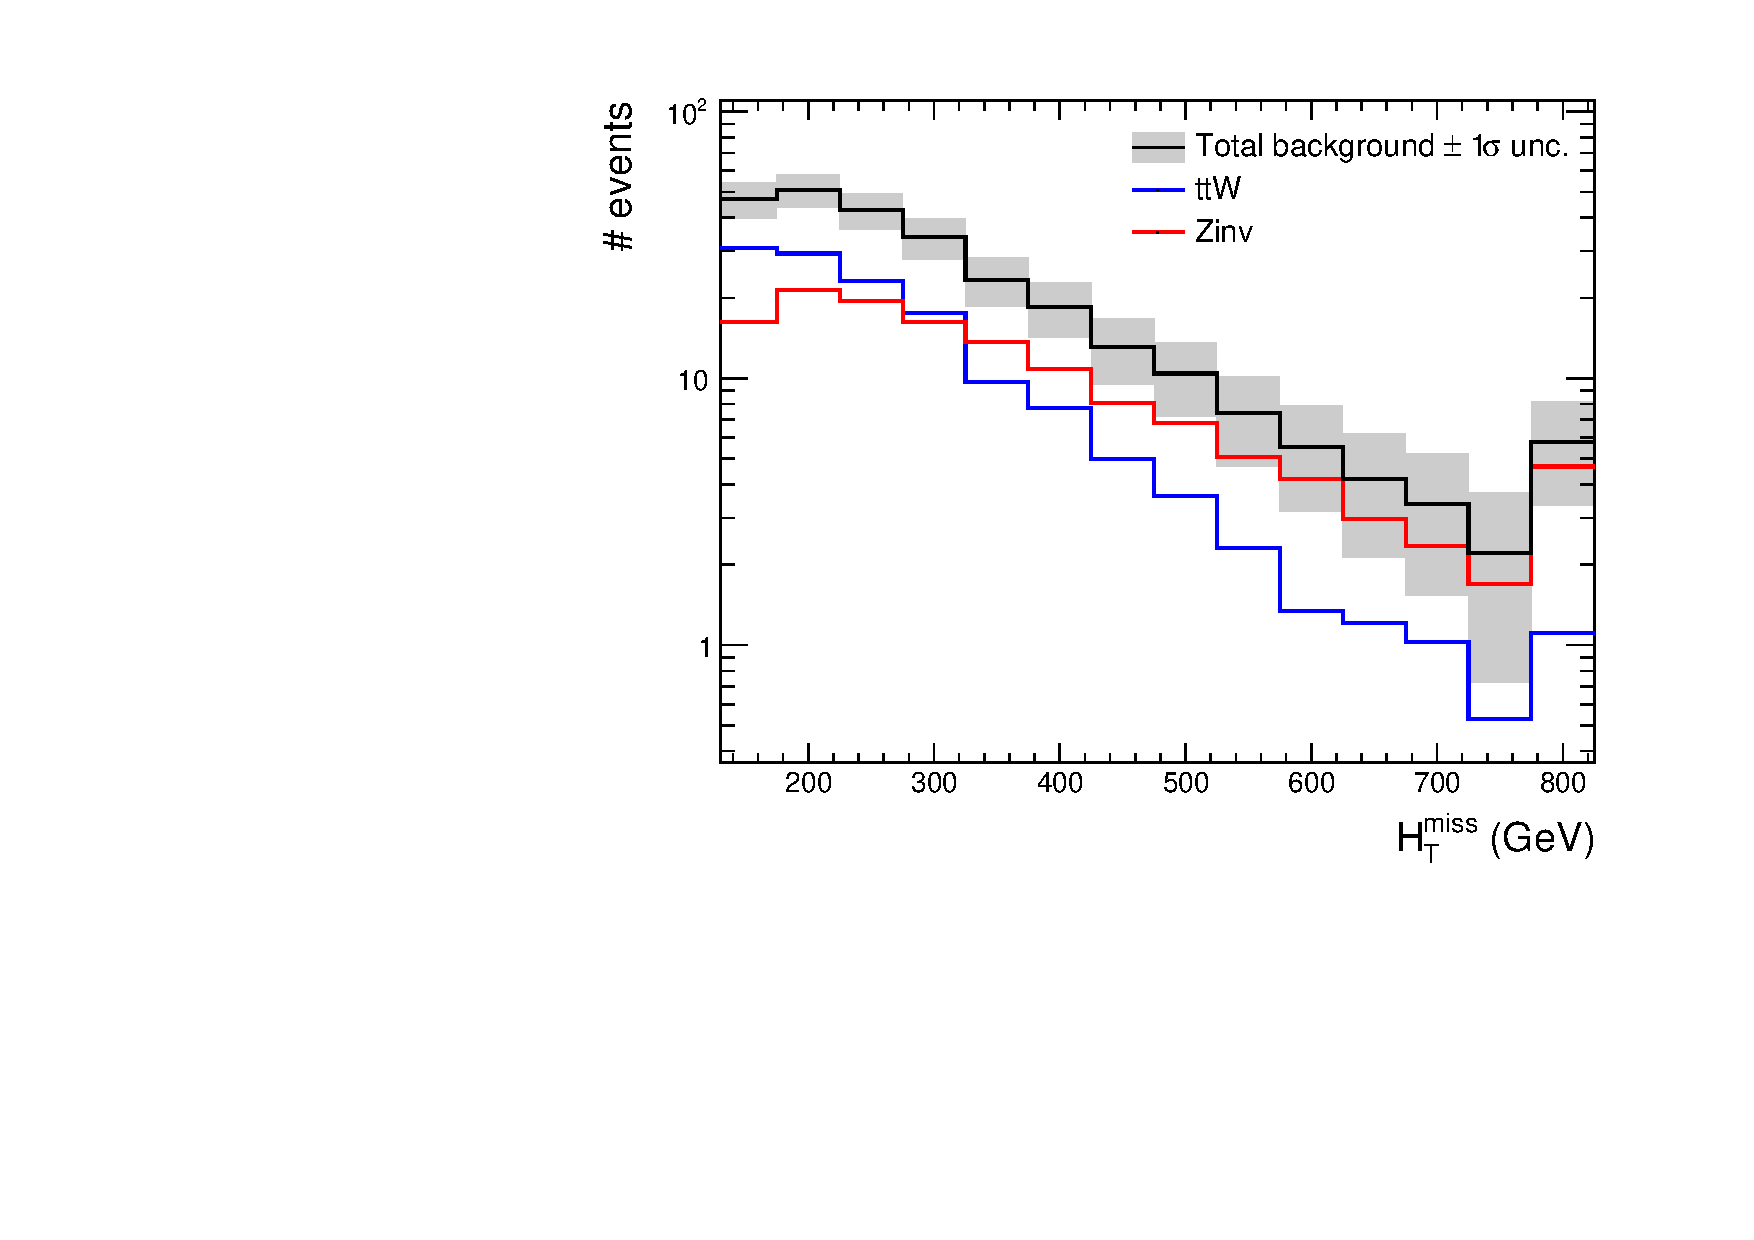
\includegraphics[width=0.5\textwidth]{figures/template/exampleTemplate13TeV.pdf}
  \\
  \caption{\label{fig:exampleTemplate13} Example template for 0b,$\ge5$j and $\scalht > 800$\GeV showing the error from both
components of the background on the total background prediction.}
  
\end{figure}

% \subsection{Additional uncertainties in the \texorpdfstring{\mht}~ dimension}
% \label{sec:addMhtUnc}
% Theoretical uncertainties due to scale differences in the data and MC agreement 
% are mitigated through the procedure described in
% Section~\ref{sec:syst-on-shape}. Other additional potential 
% sources of uncertainty will be considered, such as
% ISR, JES, PDF, b-tag scale factors, etc, as detailed below. In
% general, for each source of systematic, the \mht templates are found
% based on $\pm$1$\sigma$ variations in the relevant source of
% uncertainty. The alternative templates reflect the magnitude of the
% migration of events between bins in \mht (but not in \njet, \nb, nor
% \scalht, which is encapsulated by the normalisation systematic
% uncertainties from closure tests). If the systematic source is found
% to be significant, the template variations will be included in the
% likelihood. 
%
% \begin{figure}[]
%   \centering
%   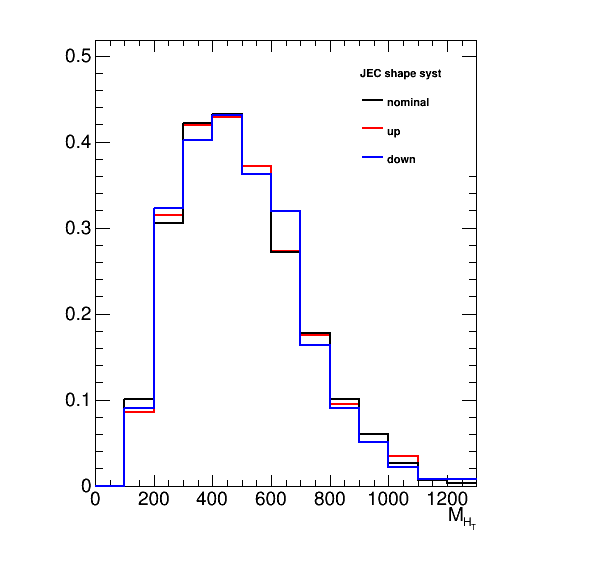
\includegraphics[width=0.5\textwidth]{figures/closureTests/mhtJetSyst_SMS_T1bbbb_2J_mGl1000_mLSP900_JEC_ge3b_ge5j_800_1600.png}
%   \caption{\label{fig:jec-shape} Alternative \mht templates that
%     reflect uncertainties in the jet energy scale corrections for
%     $\geq$5 jets, $\geq$3 b-jets, and $\scalht > 800\gev$ bin for the
%     10 \ifb luminosity scenario.}
% \end{figure}
%
% An indicative behaviour is shown in Figure~\ref{fig:jec-shape} by
% considering the variation of jet energy scale given the uncertainties
% determined in Run~1. The relative change in the \mht distribution is
% determined when varying the energy of all jets in an event up or down
% according to a \pt- and $\eta$-dependent jet energy scale uncertainty
% (\ie vary the event scale up and down), as recommended by the JetMET
% POG. 

% \begin{figure}[]
%   \centering
%   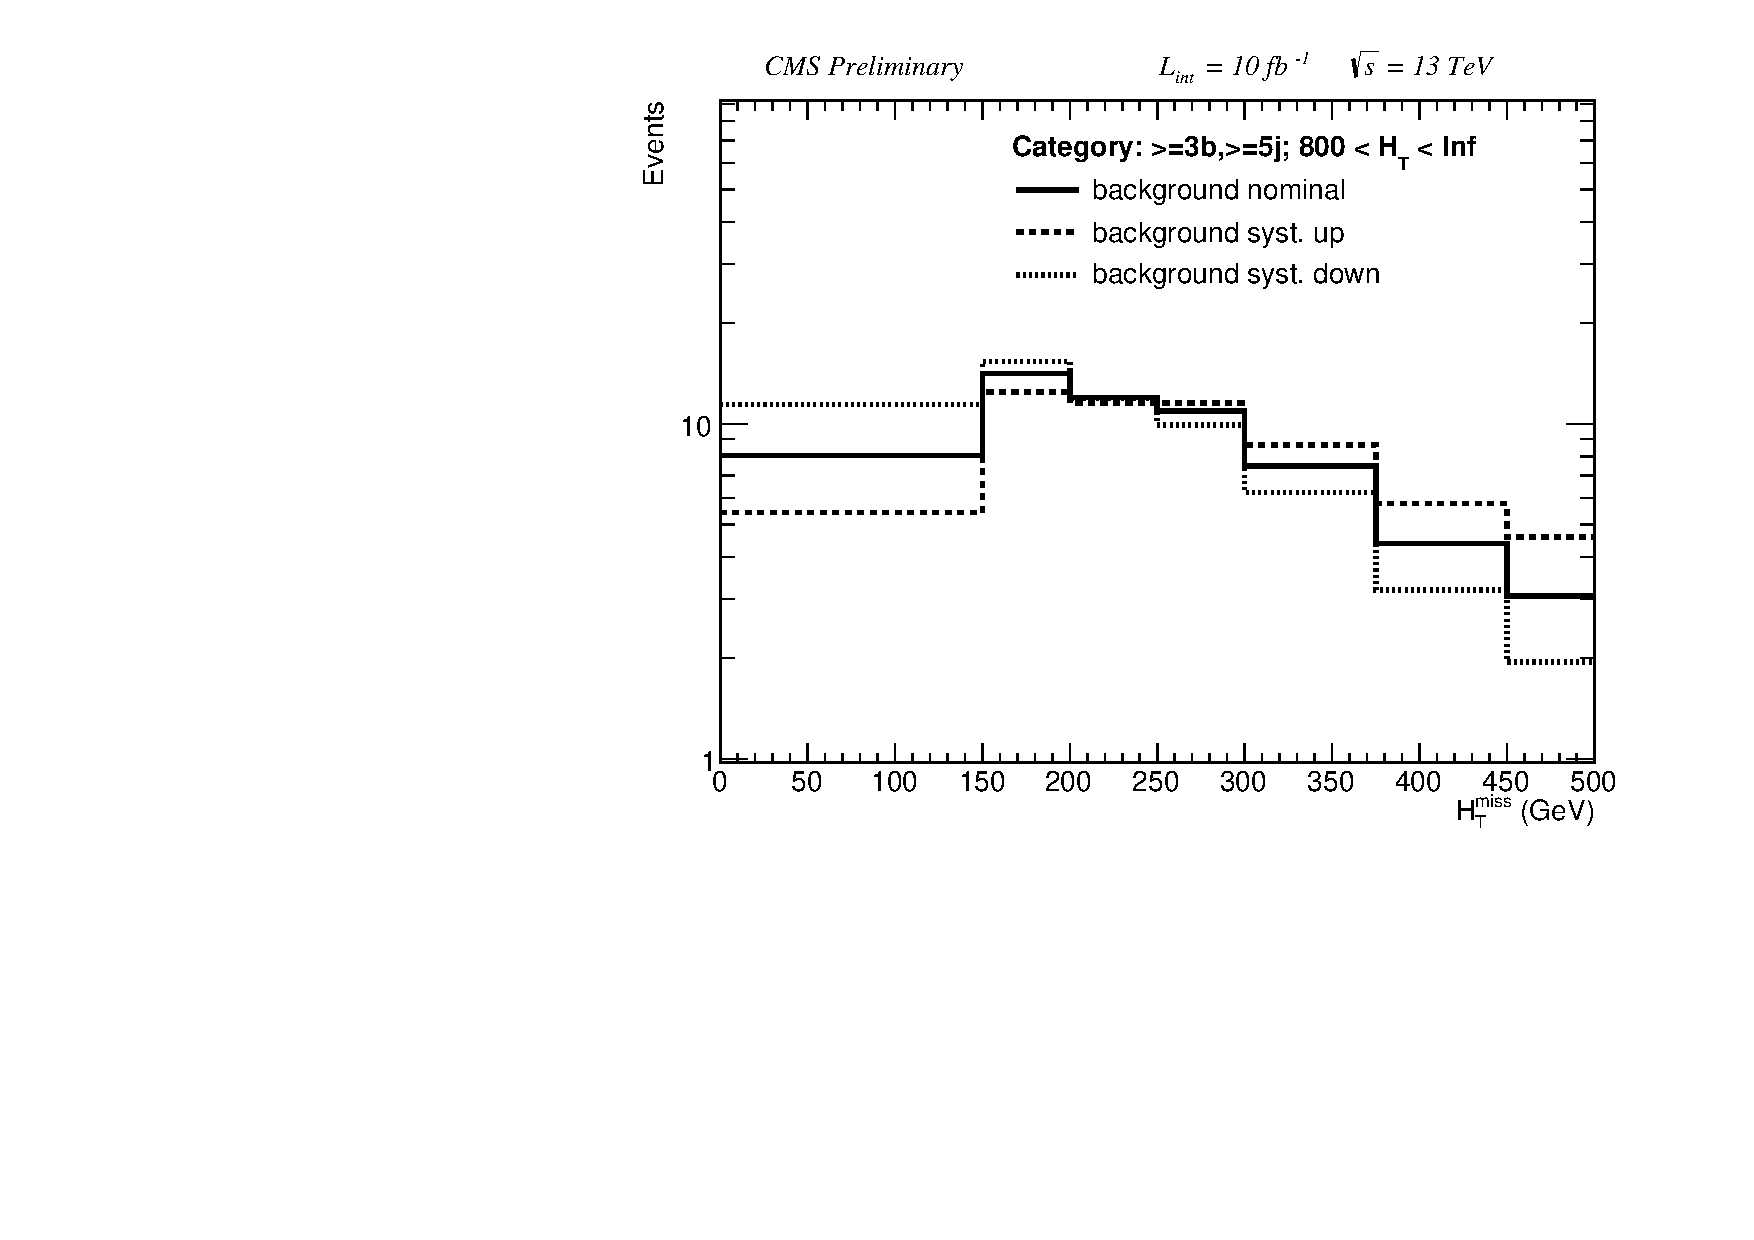
\includegraphics[width=0.7\textwidth]{figures/mhtShapeSyst/MHTShapeSyst_ge3b_ge5j_800_Inf.pdf}
%   \caption{\label{fig:mht-shape-syst-toy} 
%     The nominal \mht shape and its up/down alternative shapes for the 
%     \ttbar/W background in the $\njet \geq5$, $\nb \geq 3$
%     category for the $\HT > 800 \gev$ bin.
%   }
% \end{figure}

% %While simulation-based studies are also ongoing, some comments are
% %made below on some of the potential sources of uncertainty that are
% %expected to be dominant. This list is clearly not exhaustive.
% %
% %{\bf Jet energy scale:} 
% %
%
% %
% %{\bf PDF uncertainties:}
% %
% %\newcommand{\lcr}{Left: $\frac{\epsilon_{CTEQ6L1}}{\epsilon_{CT10}}$,
% %  center: $\frac{\epsilon_{CTEQ6L1}}{\epsilon_{MSTW08}}$, right:
% %  $\frac{\epsilon_{CTEQ6L1}}{\epsilon_{NNPDF2.1}}$}
% %
% %The samples are produced with the \verb!CTEQ6L1! PDF set by default.
% %The shape is compared with that obtained with three alternative PDF
% %sets: \verb!CT10!, \verb!NNPDF2.1!, and \verb!MSTW2008!. The envelope
% %and its uncertainties are determined following the PDF4LHC
% %recommendation~\cite{pdf4lhc}. 
% %
% %{\bf Initial state radiation:}
% %
% %Will have to cook up a recipe for this\ldots
% %
% %
% %{\bf \texorpdfstring{\mht/\met}{MHT/MET} cleaning cut:}
% %
% %The efficiencies for the requirement $\mht/\met < 1.25$ must be
% %measured in data and simulation as a function of \mht for each \scalht
% %bin. The ratio of these two efficiencies should be unity. Deviation
% %from unity is taken to represent the uncertainties on the simulation
% %modelling of this variable for processes with significant, genuine
% %\met. This can be used to define templates for the uncertainty on this
% %quantity.
% %
% %{\bf Dead ECAL filter:}
% %
% %The ratio of efficiencies observed in data and simulation for the dead
% %ECAL filter may be used as in Section~\ref{sec:sms-syst-mht-met} to
% %templates for the uncertainty from the Dead ECAL filter.
